%
%---Beginning of Document---
%
% Use 1). latex ctof-nim.tex, 2). dvipdfm ctof-nim
%
%\RequirePackage{lineno}
\documentclass{elsart}
\usepackage[dvips]{color,graphics}
\usepackage[pdftex]{graphicx}
%\setcounter{footnote}{0}
\setcounter{tocdepth}{2}
%
\usepackage{lineno} 
\linenumbers

\begin{document}
\begin{frontmatter}

\title{The Central Time-of-Flight System for CLAS12}

\author[JLAB]{D.S. Carman\thanksref{corresponding}},
\author[JLAB]{G. Asryan},
\author[JLAB]{V. Baturin},
\author[Glasgow]{L. Clark}
\author[INFN]{R. De Vita}
\author[KNU]{W. Kim}, 
\author[JLAB]{B. Miller},
\author[KNU]{A. Ni}, and
\author[JLAB]{C. Wiggins} 

\address[JLAB]{Thomas Jefferson National Accelerator Facility, Newport News, VA 23606, USA}
\address[Glasgow]{University of Glasgow, Glasgow G12 8QQ, United Kingdom}
\address[INFN]{INFN, Sezione di Genova, 16146 Genova, Italy}
\address[KNU]{Kyungpook National University, Daegu 41566, Republic of Korea} 
\thanks[corresponding]{Corresponding author. Address: 12000 Jefferson Ave., Newport News, VA; 
e-mail: carman@jlab.org.}

\date{\today}

%\maketitle

\begin{abstract}
The Central Time-of-Flight system for the large-acceptance CLAS12 spectrometer in Hall~B at 
the Thomas Jefferson National Accelerator Facility is described. The system consists of a 
hermetic barrel of scintillation counters at a radius of 25~cm from the beamline. The 
wedge-shaped counters are roughly 3.4~cm wide, 3.0~cm thick, and 90~cm long, and span a range 
of polar angles relative to the center of the nominal target location from roughly 35$^\circ$ 
to 125$^\circ$. The counters reside in the 5-T field of the CLAS12 superconducting solenoid. 
The bars are read out via bent light guides 1~m long on the upstream end of the counters and 1.6~m
long on the downstream end. The phototubes are shielded by a multi-layer dynamical magnetic shield
system to reduce the local fringe fields in the range from 400~G to 1000~G down to the level of 0.2~G
at the location of the photocathodes. The average intrinsic time resolution of the counters is 65~ps.
\end{abstract}

\end{frontmatter}

PACS:29.40.Mc \\
Keywords: CLAS12, time of flight, plastic scintillator, particle identification
\newpage

\newpage
\tableofcontents

\newpage
\section{Overview of CLAS12}

The Thomas Jefferson National Accelerator Facility (JLab) recently completed a project to 
double the maximum energy of its electron accelerator from 6~GeV to 12~GeV. The experimental 
equipment in Hall~B forms the large-acceptance CLAS12 spectrometer that was designed to operate 
with beam energies up to 11~GeV at a nominal beam-target luminosity of 
$1 \times 10^{35}$~cm$^{-2}$s$^{-1}$ to allow for precision measurements of exclusive 
reactions with polarized beam and both unpolarized and polarized targets. This spectrometer is 
based on two superconducting magnets, a solenoid in the central region about the target and a 
toroid at forward angles.

The CLAS12 torus has a six-fold symmetry that divides the forward acceptance in the range from
5$^\circ$ to 35$^\circ$ into six 60$^\circ$-wide sectors. It produces a field primarily in the 
azimuthal direction. The field strength at its nominal full current in terms of 
$\int \!B d\ell$ is 2.8~T at 5$^\circ$ and 0.5~T at 35$^\circ$. A set of three multi-layer drift 
chambers in each sector (before the field, within the field, and after the field) and a forward
micromegas vertex tracker are used for charged particle tracking to measure momenta. Downstream 
of the torus each sector is instrumented with a Cherenkov counter for $\pi/K$ separation (five 
sectors are instrumented with low threshold gas Cherenkov counters and one sector is instrumented 
with a ring-imaging Cherenkov counter), a scintillation counter wall for charged particle 
timing measurements, and an electromagnetic calorimeter system for electron and neutral particle 
identification. Just upstream of the torus is a large-volume high-threshold gas Cherenkov counter 
for electron identification and a tagging system to detect electrons and photons at scattering 
angles below $5^\circ$.

The CLAS12 solenoid spans the central angular range from 35$^\circ$ to 125$^\circ$ and has a 
uniform 5~T central field. The solenoid serves to focus the low-energy M{\o}ller background down 
the beam pipe to the beam dump away from the acceptance of the spectrometer. The detectors
mounted within the solenoid include a thick scintillation counter barrel for neutron identification, a
barrel of thin scintillation counters for charged particle timing measurements called the Central 
Time-of-Flight (CTOF) system, and a set of tracking detectors about the target.

Fig.~\ref{clas12-model} shows a three-dimensional representation of CLAS12 from the design model
to highlight the layout and the scale of the spectrometer. The CLAS12 spectrometer was installed 
and instrumented in Hall~B in the period from 2012 to 2018. The CLAS12 spectrometer took the place 
of the original CLAS spectrometer~\cite{clas-nim} that operated in Hall~B in the period from 1997 
to 2012 when it was decommissioned.

%%%%%%%%%%%%%%%%%%%%%%%%%%%%%%%%%%%%%%%%%%%%%%%%%%%%%%%%%
\begin{figure}[htbp]
\vspace{5.7cm}
\begin{picture}(50,50) 
\put(20,250)
{\hbox{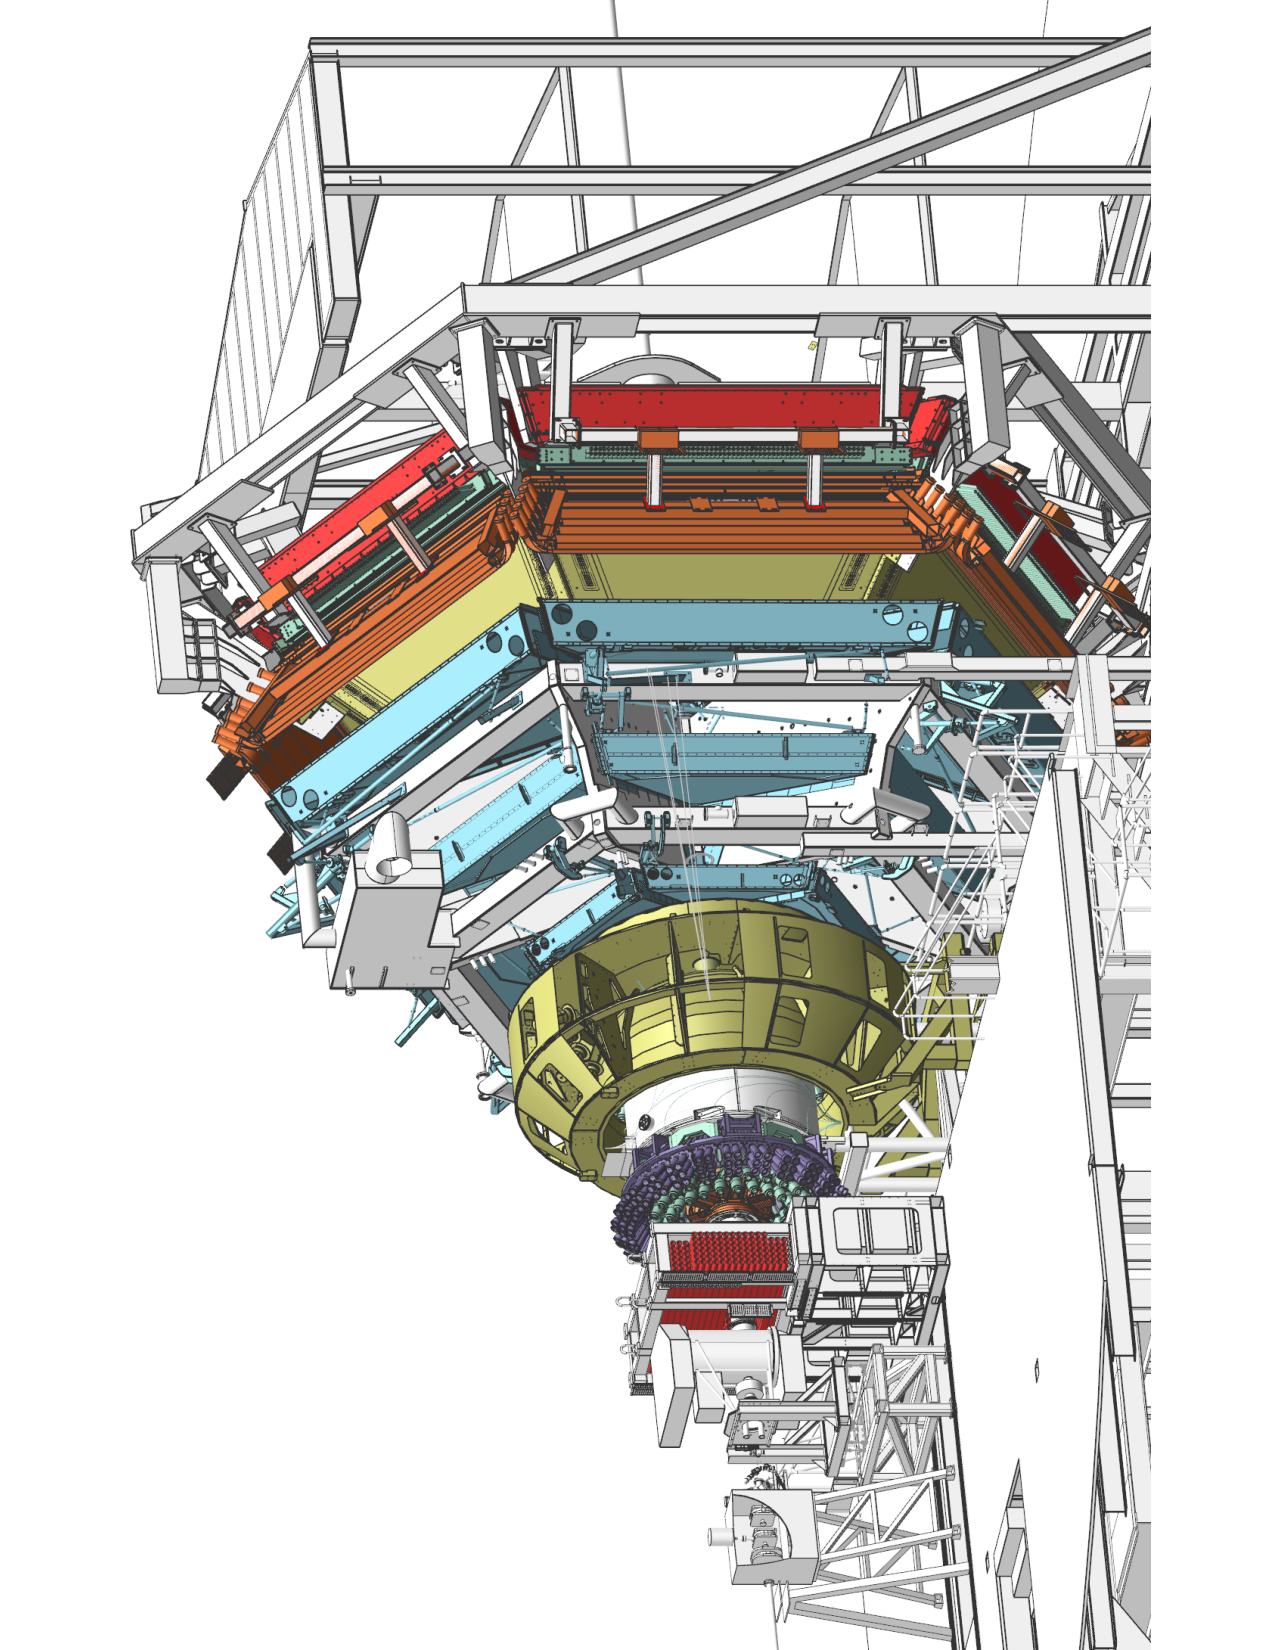
\includegraphics[width=0.70\textwidth,natwidth=610,natheight=642,angle=-90]{pics/ctof_clas12.pdf}}}
\end{picture} 
\caption{(Color Online) Model representation of the CLAS12 spectrometer in Hall~B at Jefferson
Laboratory. The electron beam is incident from the left side of this figure. The CLAS12 detector
is roughly 10~m in scale along the beam axis. For further details on the individual subsystems that
make up the CLAS12 spectrometer see Ref.~\cite{clas12-nim}.}
\label{clas12-model}
\end{figure}
%%%%%%%%%%%%%%%%%%%%%%%%%%%%%%%%%%%%%%%%%%%%%%%%%%%%%%%%%

This paper focuses on the CLAS12 CTOF detector system and is organized as follows: 
Section~\ref{sec:overview} provides a high-level overview of the CTOF system and its design 
requirements, Section~\ref{sec:design} provides a technical description of the system design, and
Section~\ref{sec:performance} highlights the performance of the system through both bench testing
with cosmic rays, as well as during the 2017 beam commissioning run and 2018 data runs. Finally,
Section~\ref{sec:summary} provides a summary regarding the CTOF detector system for CLAS12.

\section{Overview of the CTOF System}
\label{sec:overview}

The CTOF system is used to measure the flight time of charged particles emerging from interactions
in the target in the angular range from 35$^\circ$ to 125$^\circ$. The system specifications call for
an average time resolution for each counter along its full length of $\sigma_{TOF}$=65~ps. The CTOF
detector surrounds the experimental target at a radial distance of 25~cm and consists of 48 90-cm-long
scintillation bars having a trapezoidal cross section to form a hermetic barrel as shown in
Fig.~\ref{ctof-design}. The barrel is positioned inside of the CLAS12 5-T superconducting solenoid
magnet just inside a set of thick scintillation counters used for neutron detection and just outside of the
central tracking system as shown in Fig.~\ref{cut-view}. This figure shows that the CTOF is mounted to
the solenoid with the beamline along the symmetry axis of the CTOF barrel. A summary of the CTOF
technical parameters is given in Table~\ref{spec-table}. 

%%%%%%%%%%%%%%%%%%%%%%%%%%%%%%%%%%%%%%%%%%%%%%%%%%%%%%%%%
\begin{figure}[htbp]
\vspace{4.3cm}
\begin{picture}(50,50) 
\put(85,175)
{\hbox{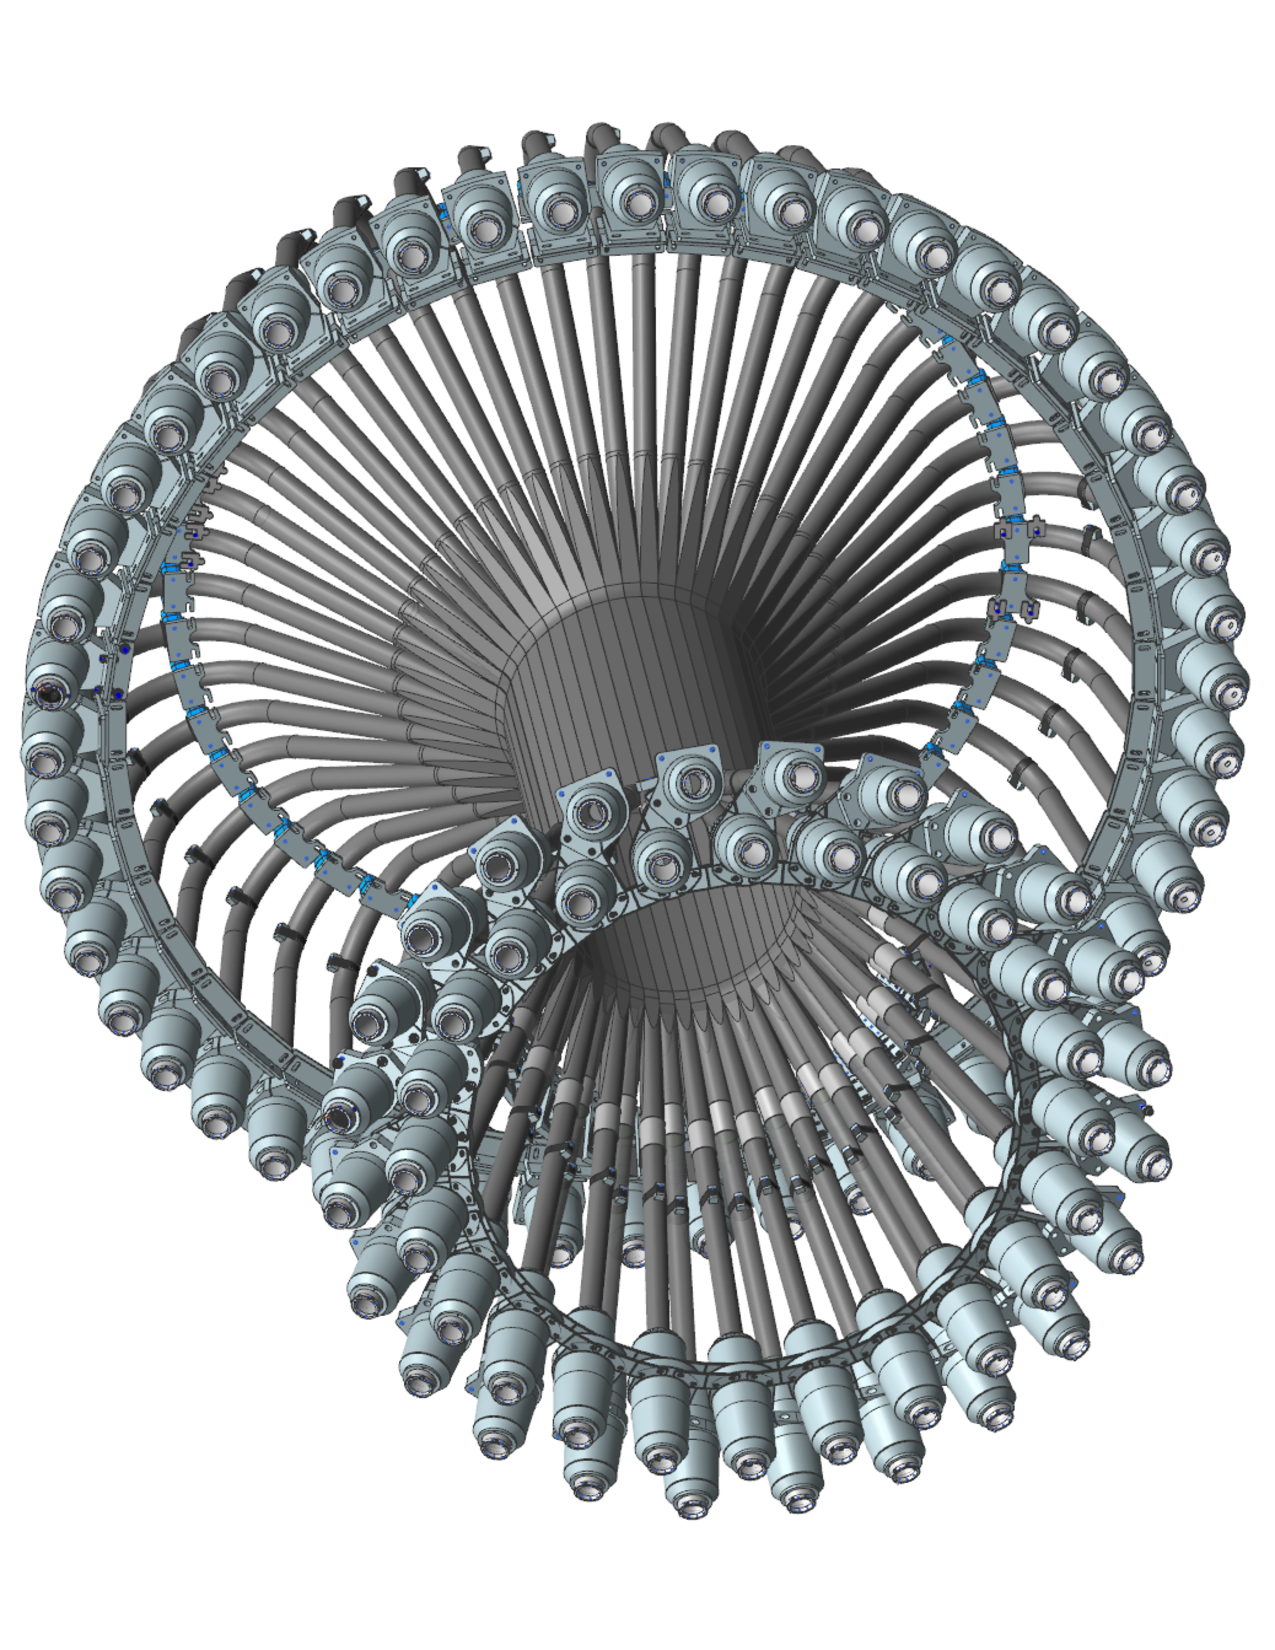
\includegraphics[width=0.45\textwidth,natwidth=610,natheight=642,angle=-90]{pics/ctof-design.pdf}}}
\end{picture} 
\caption{(Color Online) View of the Central Time-of-Flight (CTOF) system for CLAS12. The scintillation
bars form a hermetic barrel and the PMTs are attached to the ends of long light guides attached to each
end of the bars. The beam enters the detector in this figure from the left side.} 
\label{ctof-design}
\end{figure}
%%%%%%%%%%%%%%%%%%%%%%%%%%%%%%%%%%%%%%%%%%%%%%%%%%%%%%%%%

%%%%%%%%%%%%%%%%%%%%%%%%%%%%%%%%%%%%%%%%%%%%%%%%%%%%%%%%%
\begin{figure}[htbp]
\vspace{6.4cm}
\begin{picture}(50,50) 
\put(60,223)
{\hbox{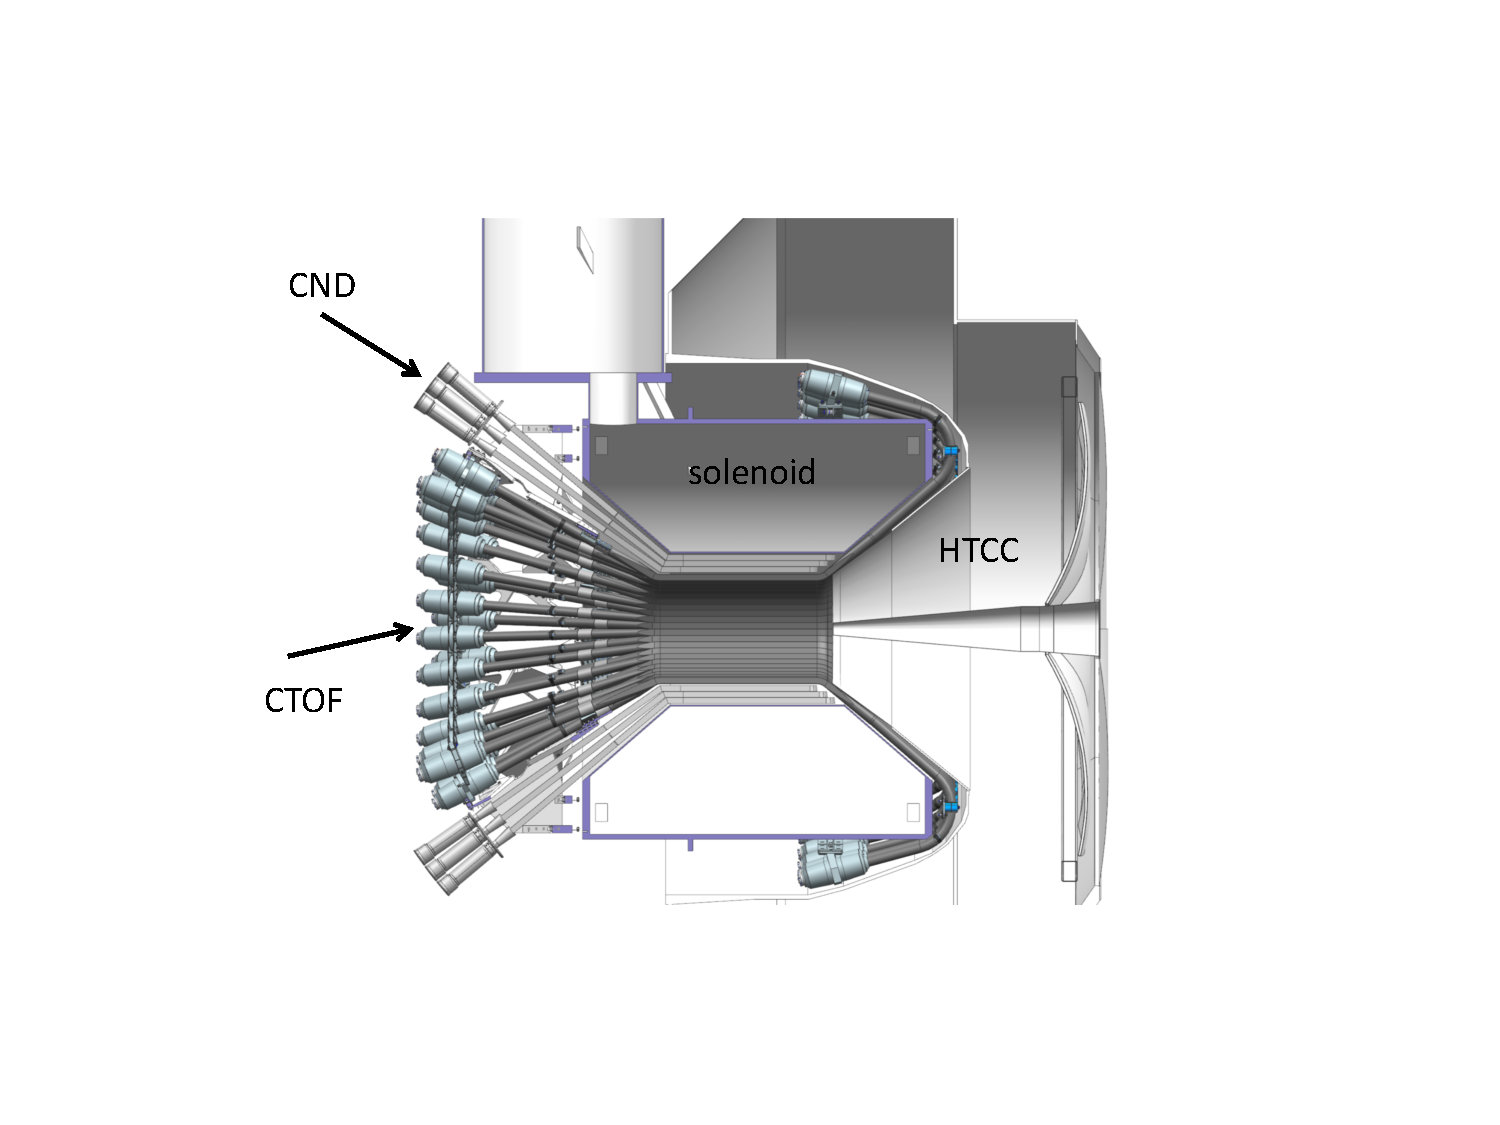
\includegraphics[width=0.55\textwidth,natwidth=610,natheight=642,angle=-90]{pics/ctof-insitu.pdf}}}
\end{picture} 
\caption{(Color Online) CTOF mounted within the CLAS12 solenoid in a cut view where the beam axis runs
along the CTOF barrel symmetry axis with the beam entering from the left. This figure shows the CTOF
counters in relation to the Central Neutron Detector and the cryostat of the superconducting solenoid.}
\label{cut-view}
\end{figure}
%%%%%%%%%%%%%%%%%%%%%%%%%%%%%%%%%%%%%%%%%%%%%%%%%%%%%%%%%

Each counter is read out via a photomultiplier tube (PMT) on each end through long light guides. As
shown in Figs.~\ref{ctof-design} and \ref{cut-view}, the upstream light guides are straight and
the downstream light guides are bent to curve around the downstream face of the solenoid magnet. 
The upstream light guides are 1~m long and the downstream light guides are 1.6~m long. These 
long light guides are necessary to position the field-sensitive PMTs in reduced regions of the
solenoid fringe field. However, even in these positions, the PMTs reside in inhomogeneous fields 
at levels as large as 1~kG at the location of the upstream PMTs and as large as 400~G at the 
location of the downstream PMTs. In order to allow for operation of the PMTs in this environment, 
they are mounted within multi-layer magnetic shields (see Section~\ref{sec:shields}).

The main requirement for the CTOF system is that its counters provide excellent timing resolution 
for particle identification. Given the nominal timing resolution of the counters, the momentum 
threshold for particle identification can be defined. These thresholds are quoted at the 3.3$\sigma$
level for CTOF, which amounts to the momenta where particle identification can occur with up to an
order of magnitude difference in the relative yields of the different species. The timing resolution is
illustrated by computing the flight time differences between different charged particle species, pions,
kaons, and protons, for tracks normally incident on the detector. Fig.~\ref{tdiff} shows the computed
time differences as a function of momentum. Where the 3$\sigma$ line crosses the computed time
difference curves defines the momentum limit for particle identification for each particle species.
These limits are quoted as 0.58~GeV for $\pi/K$ separation, 0.93~GeV for $K/p$ separation, and
1.14~GeV for $\pi/p$ separation (see Table~\ref{spec-table}). The minimum momentum acceptance
for CTOF is roughly 300~MeV as lower momentum tracks are curled up in the solenoid field and never
reach the inner surface of the CTOF counters.

%%%%%%%%%%%%%%%%%%%%%%%%%%%%%%%%%%%%%%%%%%%%%%%%%%%%%%%%%
\begin{figure}[htbp]
\vspace{5.0cm}
\begin{picture}(50,50) 
\put(35,-100)
{\hbox{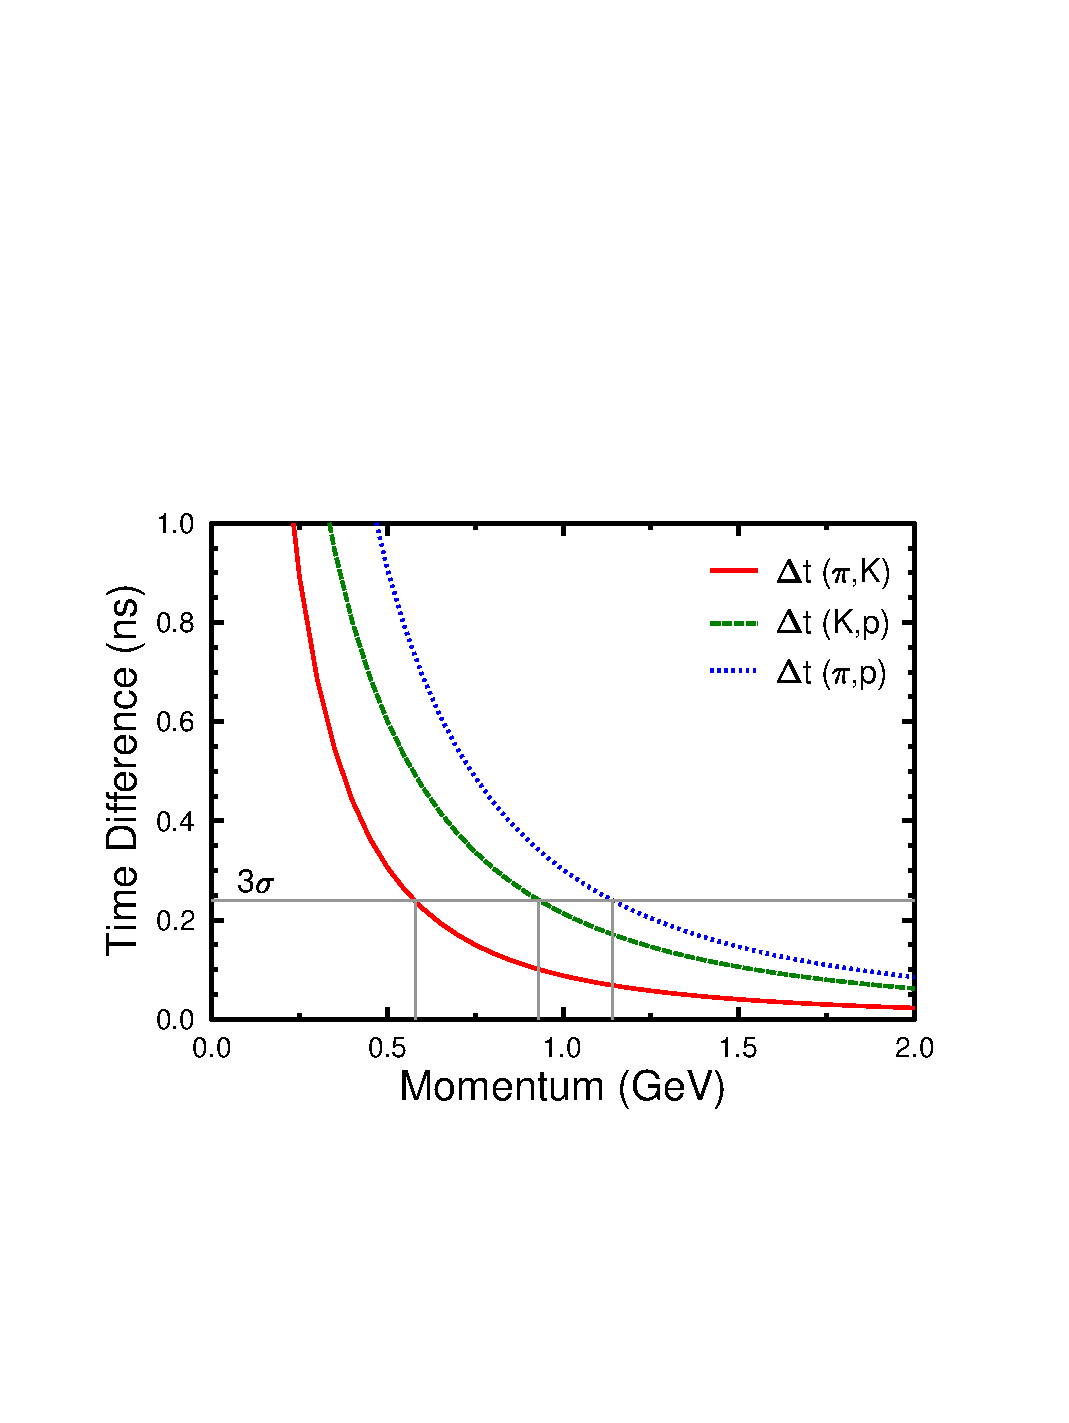
\includegraphics[width=1.00\textwidth,natwidth=610,natheight=642]{pics/tdiff_alt.pdf}}}
\end{picture} 
\caption{(Color Online) Plot of time difference between different charged particle species as a function
of momentum for normally incident tracks. The momentum at the time difference separation of 3$\sigma$
gives a measure of the particle identification capabilities of the CTOF system. The minimum momentum for
tracks to reach the CTOF system is roughly 300~MeV.}
\label{tdiff}
\end{figure}
%%%%%%%%%%%%%%%%%%%%%%%%%%%%%%%%%%%%%%%%%%%%%%%%%%%%%%%%%

Fig.~\ref{pth-kin} shows a plot of the momentum versus polar angle for pions in CLAS12 from beam data
of an 11~GeV electron beam incident on a hydrogen target. Here it is seen that the typical track momenta
accepted by CTOF are in the range below 2~GeV.

%%%%%%%%%%%%%%%%%%%%%%%%%%%%%%%%%%%%%%%%%%%%%%%%%%%%%%%%%
\begin{figure}[htbp]
\vspace{4.8cm}
\begin{picture}(50,50) 
\put(95,-50)
{\hbox{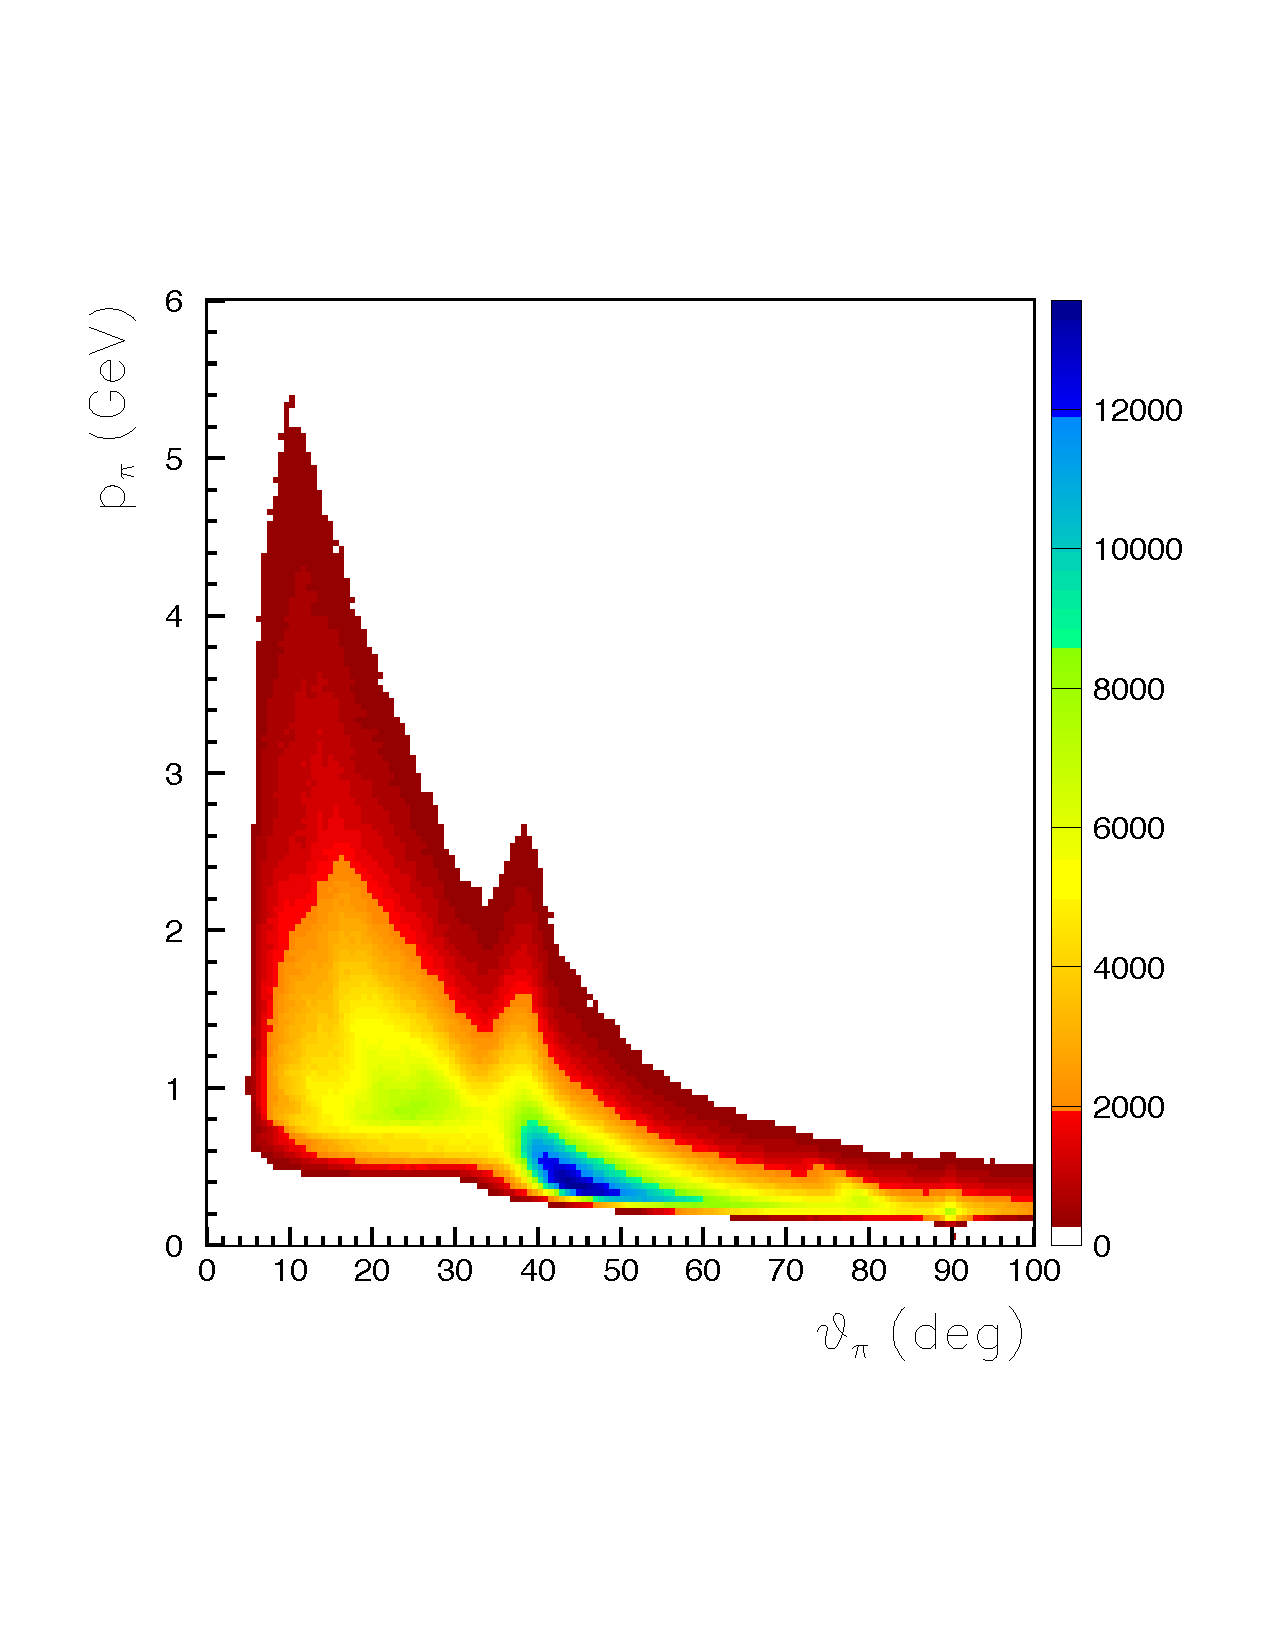
\includegraphics[width=0.55\textwidth,natwidth=610,natheight=642]{pics/pthpi.pdf}}}
\end{picture} 
\caption{(Color Online) Plot of momentum vs. polar angle for charged pions in CLAS12 from beam data
for a 10.6~GeV electron beam incident upon a liquid-hydrogen target. The discontinuity at $\theta=35^\circ$
is due to the small acceptance gap between the Forward and Central Detectors. The typical momentum
of charged tracks in the Central Detector is less than 2~GeV.}
\label{pth-kin}
\end{figure}
%%%%%%%%%%%%%%%%%%%%%%%%%%%%%%%%%%%%%%%%%%%%%%%%%%%%%%%%%

The scintillation counter signals are used in the CLAS12 Level~1 trigger to define charged hadrons in
the Central Detector, as well as to provide an effective charged particle veto for the neutron detector
system located radially outward of the CTOF. The CTOF system must, therefore, provide signals
representing a uniform response with adequate granularity to select particles reaching the CTOF
detectors. The pulse height information from the CTOF system is also used for energy-loss measurements
to provide supplemental means for the identification of slow particles.

%%%%%%%%%%%%%%%%%%%%%%%%%%%%%%%%%%%%%%%%%%%%%%%%%%%%%%%%%
\begin{table}[htbp]
\begin{center}
\begin{tabular} {ll} \hline
~~Parameter~~ &~~~~~~~~~~~~~~~~~~~~~~ Design Value ~~~~~~~~~~\\ \hline
Counters             & Barrel of 48 EJ-200 bars; double-ended readout \\
Angular Coverage     & $\theta$: (35$^\circ$,125$^\circ$), $\phi$: (-180$^\circ$,180$^\circ$) \\
Counter Dimensions   & Trapezoidal cross section $\sim 3.4 \times 3.0 \times 90$~cm$^3$ \\
PMTs                 & Hamamatsu R2083 (H2431-MOD assembly)    \\
Upstr. Light Guides  & O.D.=5.08~cm, 1-m-long, focusing design, straight \\
Dnstr. Light Guides  & O.D.=5.08~cm, 1.6-m-long, focusing design, bent 135$^\circ$ \\
Magnetic Shields     & 3 ferromagnetic layers with inner compensation coils \\
Timing Resolution    & 65~ps / 80~ps\\
$\pi$/$K$ separation & 3$\sigma$ up to 0.58~GeV \\ 
$K$/$p$ separation   & 3$\sigma$ up to 0.93~GeV \\ 
$\pi$/$p$ separation & 3$\sigma$ up to 1.14~GeV \\ \hline
\end{tabular}
\end{center}
\caption{CTOF technical design parameters.}
\label{spec-table}
\end{table}
%%%%%%%%%%%%%%%%%%%%%%%%%%%%%%%%%%%%%%%%%%%%%%%%%%%%%%%%%

With the limited radial extent within the 100~cm diameter solenoid, the thickness of the CTOF
scintillation bars was limited to $\sim$3~cm. In order to accommodate the target and the central
tracking system, the CTOF was positioned at a radius from the beamline of 25~cm. To ensure maximal
$\phi$ acceptance, the individual CTOF counters have a wedge-shaped geometry to form a hermetic
barrel. The width of the counters of $\sim$3.4~cm was selected to ensure that the maximum counting
rates did not exceed 500~kHz per counter with the solenoid at its nominal full field and a 
beam-target luminosity of 1$\times$10$^{35}$~cm$^{-2}$s$^{-1}$.

\section{Design of the CTOF System}
\label{sec:design}

The CTOF barrel is composed of 48 wedge-shaped scintillation bars roughly 90-cm long, read out
through 1-m-long (upstream) and 1.6-m-long (downstream) Acrylic light guides attached to the 
ends of the bars. Extensive experience with the design and calibration of the scintillation bars for 
the CLAS spectrometer (15~cm wide by 5~cm thick)~\cite{tof-nim} and for the forward angle 
time-of-flight system for CLAS12 (6~cm wide by 6~cm thick)~\cite{ftof-nim}, has shown that for 
1-m-long rectangular scintillation counters without light guides, intrinsic average timing resolutions
in the range from 40~ps to 80~ps can be achieved after all corrections are included. For the CTOF
design with its roughly 3.4~cm by 3.0~cm scintillation bars and long light guides, studies of prototype
counters showed that an average time resolution of $\sim$65~ps could be achieved only after careful
optimization of the overall system design~\cite{baturin-2009}.

The design timing resolution for the individual CTOF counters includes contributions intrinsic to the
CTOF system itself and contributions from other CLAS12 subsystems. The intrinsic resolution
is determined mainly by the number of photons created in the scintillation bar by passing charged
particles that ultimately propagate to the photocathodes of the PMTs. Due to the geometry of the
scintillation bar and the light guides, there are attenuation losses of the created light. As well, the
photons that propagate to the PMTs are dispersed in time via the different paths that they travel.
The response of the PMT, including variations in response across the photocathode, causes further
dispersion of the times of the created photoelectrons reaching the accelerating structure of the PMT.
Each of these effects must be folded in with the additional signal dispersion as it is produced along the
accelerating structure of the PMT to produce the signal pulse that is used for the time measurement.
These contributions determine the intrinsic resolution of the counter assembly. For our purposes we also
include the accounting of the intrinsic resolution effects from signal dispersion along the readout signal
cables and the resolution smearing of the readout electronics. These resolutions were determined during
our bench test measurements detailed in Section~\ref{sec:bench}. However, the overall effective resolution
of the system also includes additional smearing effects from other CLAS12 subsystems that are required
as input to calibrate the CTOF response. This includes accurate determination of the track path length and
reaction vertex point from the central tracking reconstruction, the event start time from the Forward
Detector, and the RF time associated with the beam bucket for the event. The overall effective resolution
measurements determined during beam studies in CLAS12 are detailed in Section~\ref{tres-beam}.
Table~\ref{spec-table} therefore includes two measures of the CTOF design timing resolution. The value
of 65~ps is our requirement for the intrinsic timing resolution and 80~ps represents the overall effective
resolution that sets the 3$\sigma$ specifications for particle identification.

In this section the design details of the scintillation bars, the light guides, the magnetic shields and the
electronics are discussed. Each component of the system design was considered within the context of the
design constraints both for the CTOF and the neighboring detector subsystems, and optimized against
cost and performance considerations. 

\subsection{Geometry}
\label{geometry}

The scintillation bars of the CTOF barrel are composed of two slightly different designs that 
alternate in azimuth. A pair of neighboring counters is shown in Fig.~\ref{counter-pair}. The 
difference between the two designs is in the upstream straight light guide and the upstream 
end of the scintillation bars where they attach to the light guide. This design feature is 
necessary to allow for sufficient spacing for the bulky magnetic shields and their associated 
support structure. The downstream elements of the design are identical for all counters.

%%%%%%%%%%%%%%%%%%%%%%%%%%%%%%%%%%%%%%%%%%%%%%%%%%%%%%%%%
\begin{figure}[htbp]
\vspace{2.6cm}
\begin{picture}(50,50) 
\put(65,168)
{\hbox{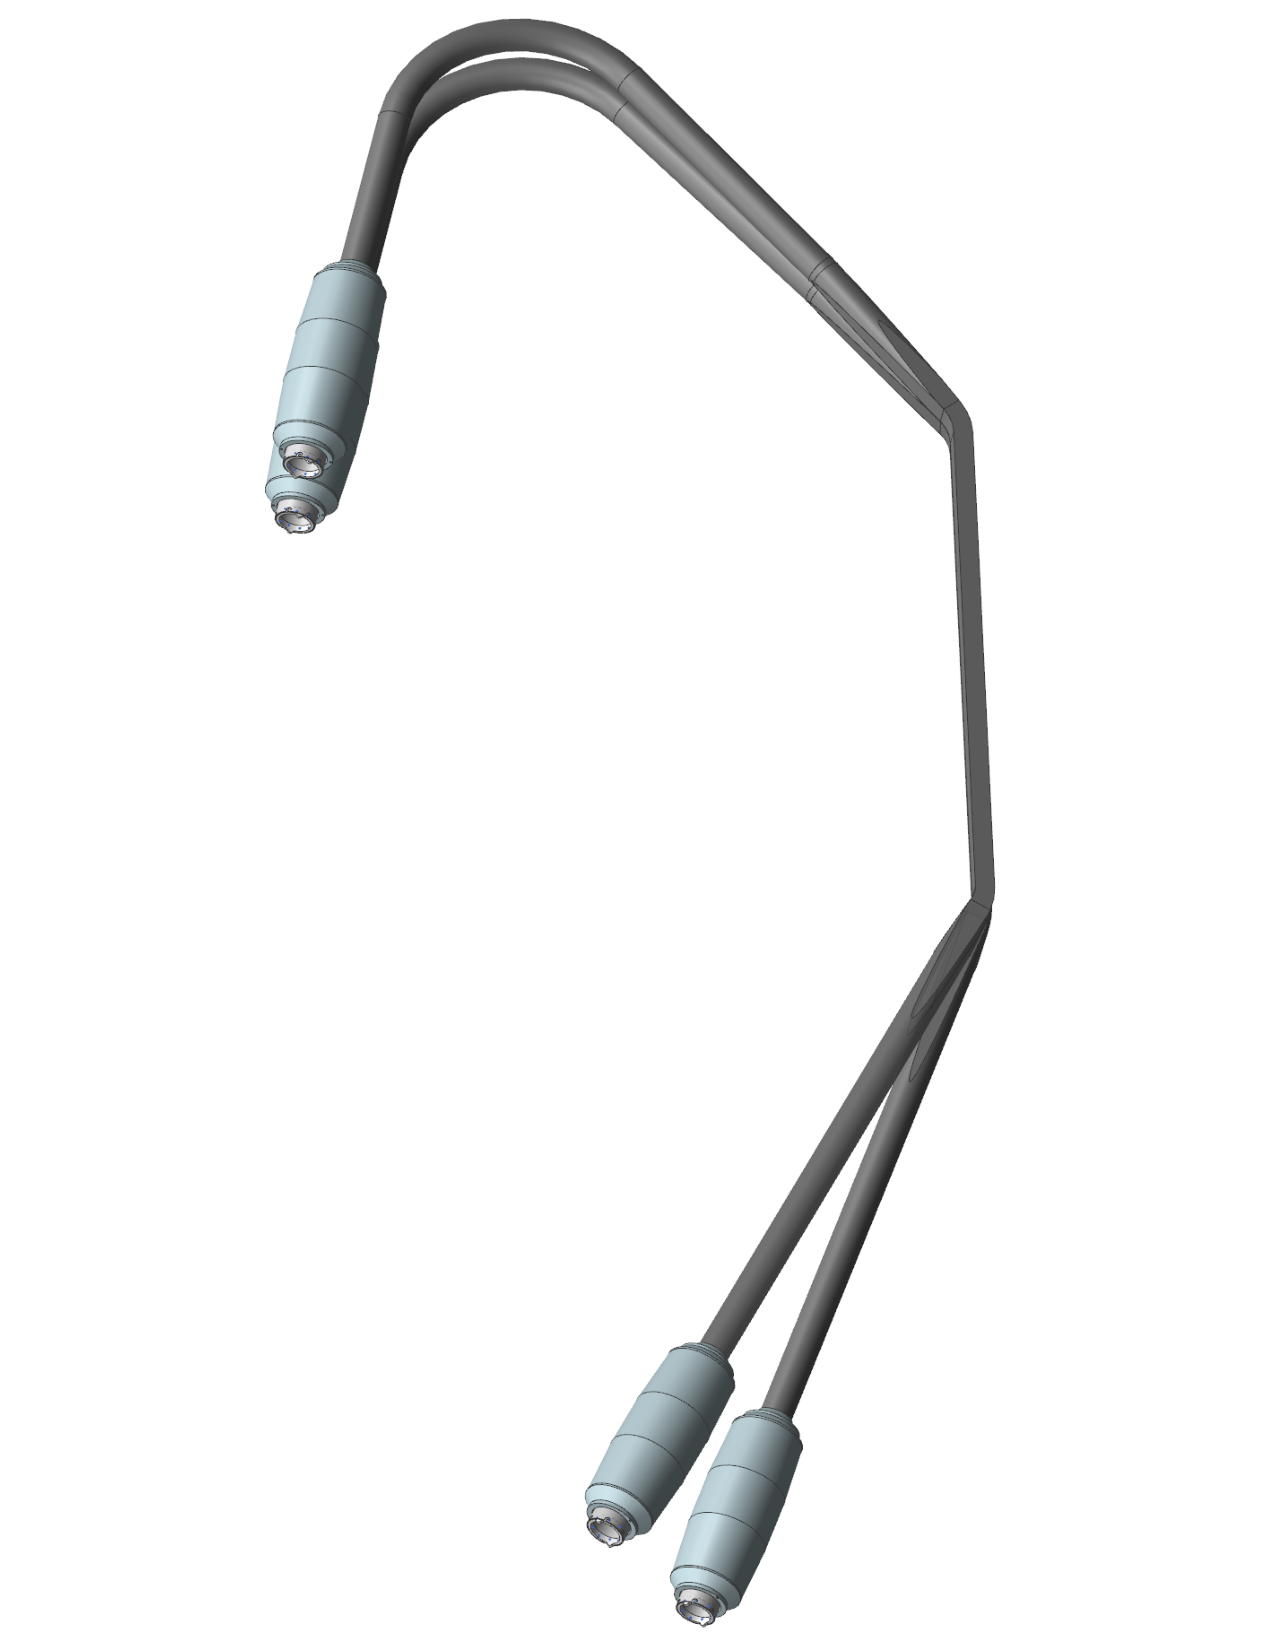
\includegraphics[angle=-90,width=0.55\textwidth,natwidth=610,natheight=642]{pics/counter-pair.pdf}}}
\end{picture} 
\caption{A pair of neighboring CTOF counters with two slightly different designs for the upstream
light guide and the upstream end of the scintillation bars.} 
\label{counter-pair}
\end{figure}
%%%%%%%%%%%%%%%%%%%%%%%%%%%%%%%%%%%%%%%%%%%%%%%%%%%%%%%%%

The two different CTOF counter designs have a slightly different pitch angle for the scintillation
bars on the upstream side. The ``low-pitch'' angle design has a pitch angle of 21.8$^\circ$ and the
``high-pitch'' angle design has a pitch angle of 29.1$^\circ$. For both the low-pitch and high-pitch
angle designs, the scintillation bars have a pitch angle at the downstream end of 36.0$^\circ$.
Fig.~\ref{scint-geom} shows a schematic side view and end view of a ``generic'' scintillation bar.

%%%%%%%%%%%%%%%%%%%%%%%%%%%%%%%%%%%%%%%%%%%%%%%%%%%%%%%%%
\begin{figure}[htbp]
\vspace{5.4cm}
\begin{picture}(50,50) 
\put(45,190)
{\hbox{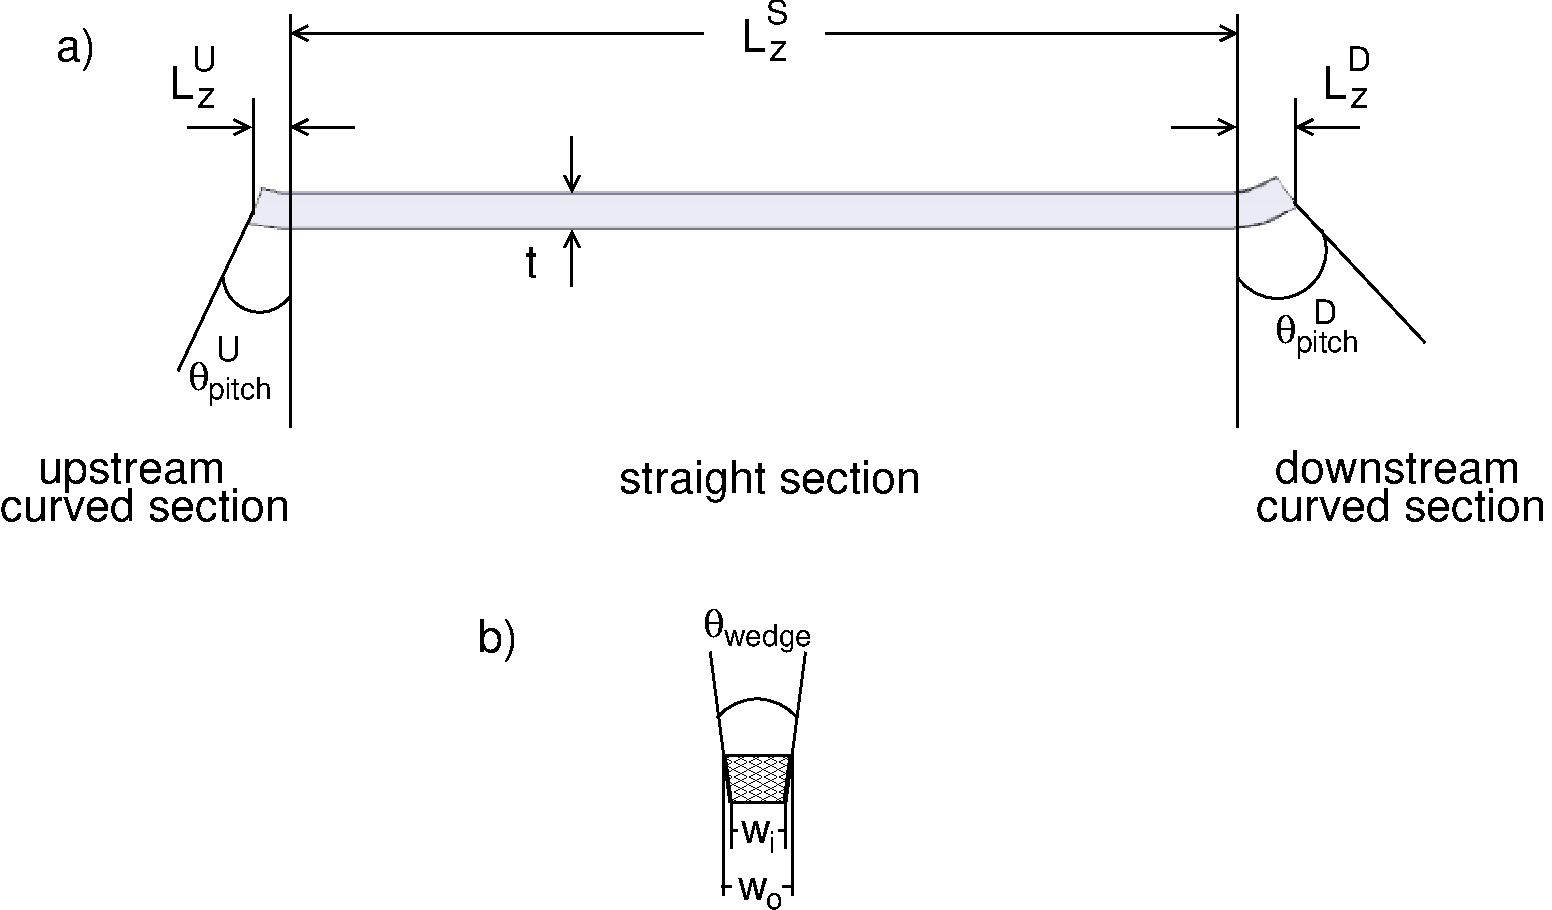
\includegraphics[angle=-90,width=0.70\textwidth,natwidth=610,natheight=642]{pics/scint-geom.pdf}}}
\end{picture} 
\caption{Schematic views of a generic CTOF scintillation bar showing a) a side view and b) 
an end view. The parameters used to define the geometry of the bar are listed. See
Table~\ref{bar-geom} for the detailed specifications.}
\label{scint-geom}
\end{figure}
%%%%%%%%%%%%%%%%%%%%%%%%%%%%%%%%%%%%%%%%%%%%%%%%%%%%%%%%%

The scintillation bar design is essentially a uniform wedge-shaped piece of scintillation material that
subtends a 7.5$^\circ$ azimuthal range as seen from the target. The very ends of the bars curve
upwards to join the light guides. A simplified description of the two different CTOF scintillation bar
designs is given in Table~\ref{bar-geom} using the variables defined in Fig.~\ref{scint-geom}. Here
$L_z$ is the section length along the beam/$z$-axis, $w_i$ ($w_o$) is the width of the scintillation bar
at its inside (outside) face, and $\theta_{wedge}$ is the azimuthal angle subtended by each bar as seen
from the target. The complete description of the scintillation bar geometry for the CTOF is made a bit
more complicated by the fact that the bars are not a uniform wedge-shaped cross section from end 
to end. They actually have a slightly projective geometry near the ends to match the designs of the light
guides but they always fit within a 7.5$^\circ$ azimuthal wedge from the target. The surface area of
the ends of each counter element $A_{end}$ is listed in Table~\ref{bar-geom}. A more complete 
description of the counter geometry is given in Ref.~\cite{geom-note}.

%%%%%%%%%%%%%%%%%%%%%%%%%%%%%%%%%%%%%%%%%%%%%%%%%%%%%%%%%
\begin{table}[htbp]
\begin{center}
\begin{tabular} {c|r|cc} \hline
Section       & Parameter          & \multicolumn{2}{c}{Design Value} \\ \hline
              &                    & Low-Pitch Angle & High-Pitch Angle \\ \cline{3-4}
Upstream      & $L_z^U$            & 2.924~cm  & 4.125~cm	  \\
              & $\theta_{pitch}^U$ & 21.8$^\circ$ & 29.1$^\circ$ \\
              & $A_{end}$          & 11.20~cm$^2$ & 12.13~cm$^2$ \\ \hline
Straight      & $L_z^S$            & \multicolumn{2}{c}{80.683~cm}    \\
              & $A_{end}$          & \multicolumn{2}{c}{10.32~cm$^2$} \\ \hline
Downstream    & $L_z^D$            & \multicolumn{2}{c}{5.624~cm}     \\
              & $\theta_{pitch}^D$ & \multicolumn{2}{c}{36.0$^\circ$} \\
              & $A_{end}$          & \multicolumn{2}{c}{11.02~cm$^2$} \\ \hline
Scintillation & $w_i$              & \multicolumn{2}{c}{3.211~cm}     \\ 
Bar           & $w_o$              & \multicolumn{2}{c}{3.607~cm}     \\  
              & $\theta_{wedge}$   & \multicolumn{2}{c}{7.5$^\circ$}  \\ 
              & $t$                & \multicolumn{2}{c}{3.022~cm}  \\ \hline   
\end{tabular}
\end{center}
\caption{Geometry specifications for the CTOF scintillation bars. See Fig.~\ref{scint-geom}
for details on the definitions of the parameters.}
\label{bar-geom}
\end{table}
%%%%%%%%%%%%%%%%%%%%%%%%%%%%%%%%%%%%%%%%%%%%%%%%%%%%%%%%%

\subsection{Scintillation Material}
\label{scint-mat}

To optimize the time resolution for the CTOF system, the scintillation bars were required to
provide a fast time response with low light attenuation. For this application EJ-200 plastic
scintillator from Eljen~\cite{eljen-ref}  was selected. This material has the same technical
specifications as for BC-408 by Bicron~\cite{bicron-ref}. EJ-200 uses polyvinyltoluene as its
base polymer. The characteristics of this material are detailed in Table~\ref{ej200-specs}.

%%%%%%%%%%%%%%%%%%%%%%%%%%%%%%%%%%%%%%%%%%%%%%%%%%%%%%%%%
\begin{table}[htbp]
\begin{center}
\begin{tabular}{lc} \hline
Light Output                  & 64\% anthracene \\
Wavelength of Max. Emission~~ & 425 nm \\
Rise Time                     & 0.9 ns \\
Decay Time                    & 2.1 ns \\
Pulse Width                   & 2.5 ns (FWHM) \\
Density                       & 1.023 g/cm$^3$ \\
Bulk Attenuation Length       & 380~cm \\
Refractive index              & 1.58 \\ \hline 
\end{tabular}
\end{center}
\caption{The properties of the plastic scintillator EJ-200 used for the CTOF scintillation bars.}
\label{ej200-specs}
\end{table}
%%%%%%%%%%%%%%%%%%%%%%%%%%%%%%%%%%%%%%%%%%%%%%%%%%%%%%%%%

The bulk attenuation length of this material is stated by its manufacturer to be $\sim$4~m. However,
the practical attenuation length of the actual prepared bars is smaller than this bulk value as the path
length of photons from the charged particle intersection point to the ends of the bar is increased due
to the finite geometry of the bar. This practical attenuation length should be longer than the bar to
ensure sufficient photon statistics at the ends of the bar. For the CTOF scintillation bars, the
manufacturing specification was that the bar attenuation length be longer than 280~cm. Measurements
of the practical attenuation length of the CTOF counters, which include the light guides, see
Section~\ref{sec:attlen} for details, are reduced from this value by a factor of two.

The scintillation bars were required to be clear and free of visual inclusions, air bubbles,
and cracks. The bars were machined with diamond-tooled end mills on two faces and were cast
against glass on the other two faces. Upon delivery the bars were subjected to additional
hand polishing to further improve the surface quality in some cases. The scintillation bar
polishing generally followed the guidelines recommended by Eljen~\cite{eljen-guide}. Using a
low-speed random orbital sander, the surface was sanded using a continuous stream of water
across the sanding head with sandpaper grits from 400 to 6000 in roughly 10 even steps. The 
bar was washed after each step with soapy water and then rinsed with water. Using a soft 
cotton cloth, a final hand polishing was then performed using alumina powders with particle 
sizes of 1~$\mu$m, 0.3~$\mu$m, and 0.05~$\mu$m, again with washing and rinsing between
each step. Care was taken in all phases of handling of the bars to wear gloves and to avoid contact 
with alcohols or other solvents.

\subsection{Light Guides}

The locations of the upstream and downstream PMTs for the CTOF system are tightly constrained
by the layout of the CLAS12 Central Detector. On the upstream end of CTOF, the PMTs must
be positioned in locations where the fringe field from the solenoid is no larger than $\sim$1~kG,
which is the practical limit of our magnetic shield design. Given the design constraints of
the tracking and target systems located radially inward of the CTOF system and the neutron
detector located radially outward of the CTOF system, as well as the necessary detector support 
structures, the upstream light guides for CTOF were required to be $\sim$1~m long and project 
away from the beamline in the angular range from 20$^\circ$ to 30$^\circ$. On the downstream 
end of CTOF, the design of the high-threshold Cherenkov detector system requires it to be 
positioned very close to the downstream face of the solenoid. This required the downstream CTOF 
PMTs to be placed on the outer surface of the solenoid magnet, which required that the downstream 
CTOF light guides curl around the downstream end of the solenoid with a minimum length of 
$\sim$1.6~m. For both the upstream and downstream light guides, the overall design principle was 
to ensure that the light guides were as short as possible to optimize the light transmittance and 
thus optimize the counter timing resolution.

The constraints on the light guides required that they match the wedge-shaped cross section
of the scintillation bar at one end and match the circular shape of the PMT at the other end,
while being restricted to lie fully within the 7.5$^\circ$ azimuthal allotment for each of the
48 counters. The CTOF light guides were manufactured by Plastic-Craft~\cite{plas-ref} from
5.08-cm diameter cast Acrylic rods ($n$=1.49). The downstream light guides were cast as straight
rods and bent on a forming mandrel after heating in a low-temperature oven. After the casting and 
machining processes, the light guides were polished to a mirror surface at the vendor with 
additional polishing performed at JLab only in the case of scratches incurred during handling.

%%%%%%%%%%%%%%%%%%%%%%%%%%%%%%%%%%%%%%%%%%%%%%%%%%%%%%%%%
\begin{figure}[htbp]
\vspace{3.0cm}
\begin{picture}(50,50) 
\put(15,130)
{\hbox{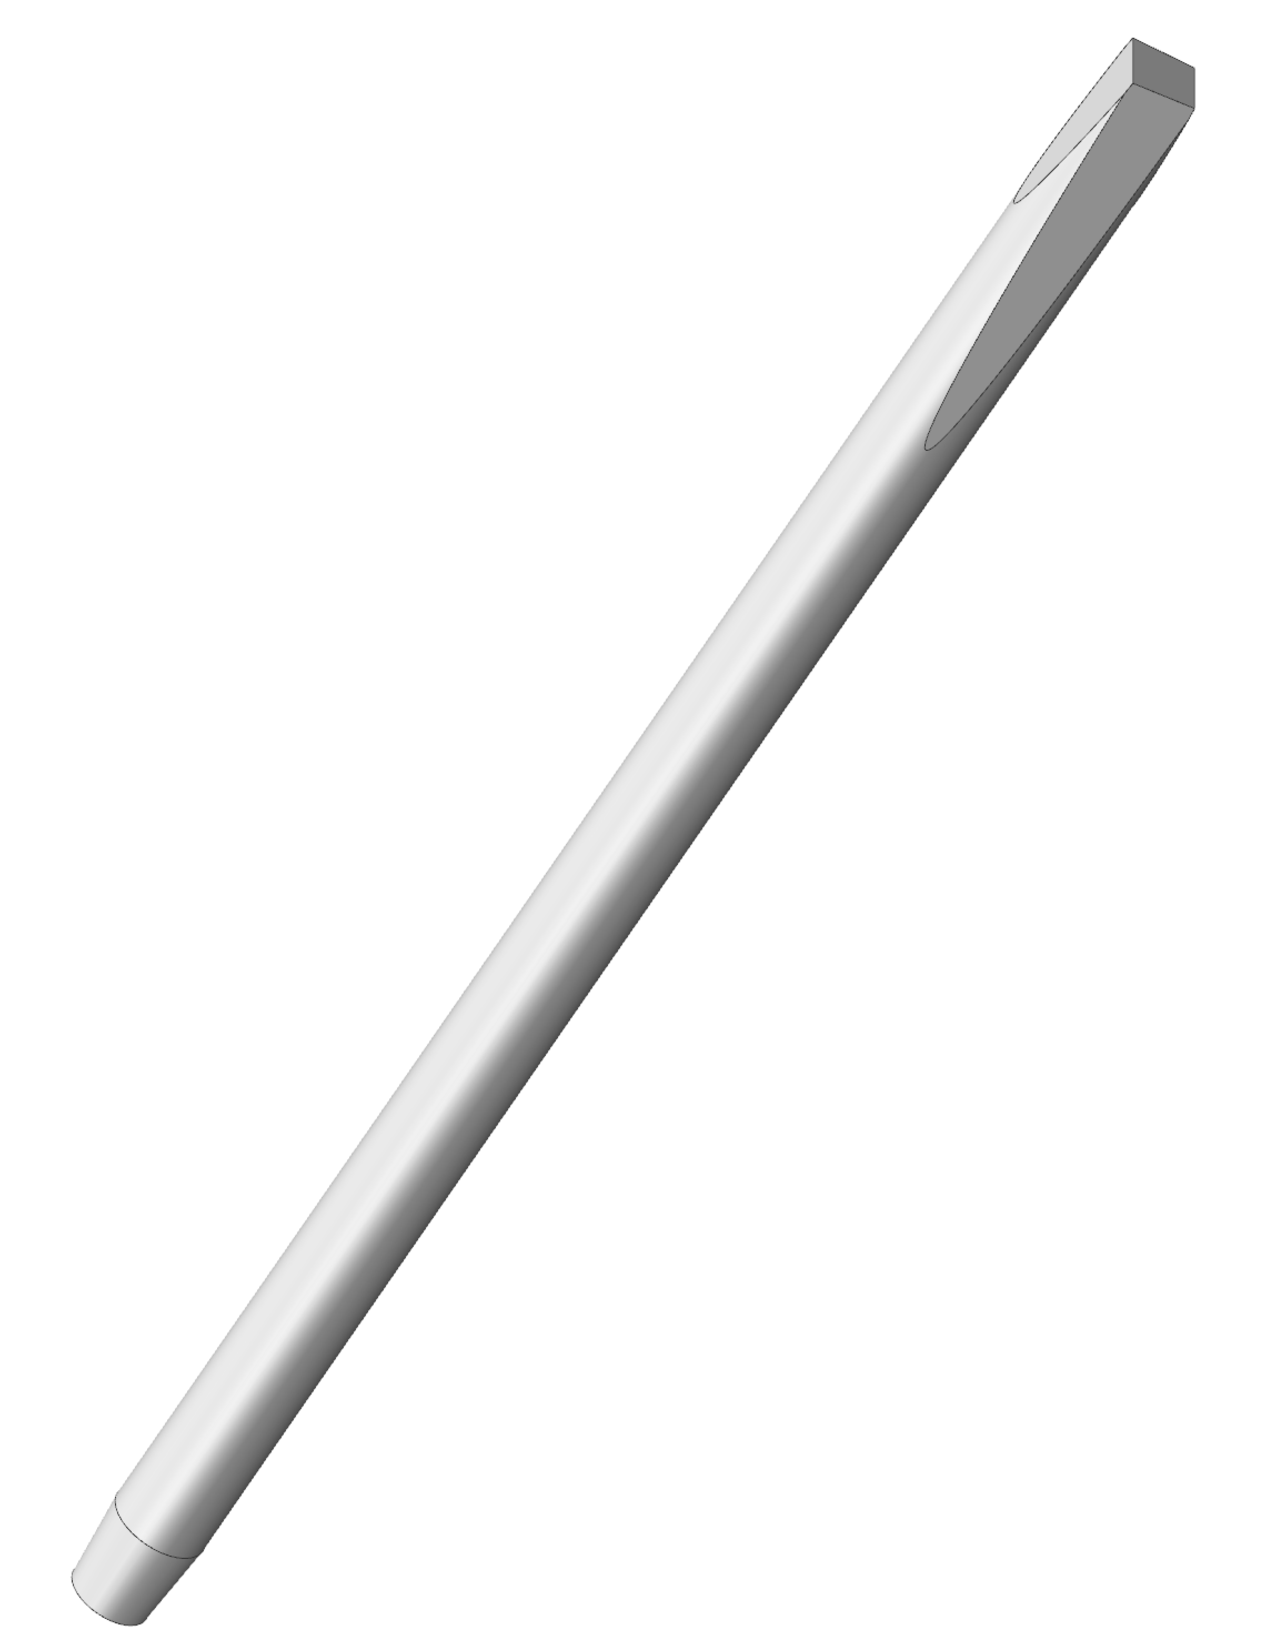
\includegraphics[width=0.35\textwidth,natwidth=610,natheight=642,angle=-90]{pics/ctof-lgu.pdf}}}
\put(170,130)
{\hbox{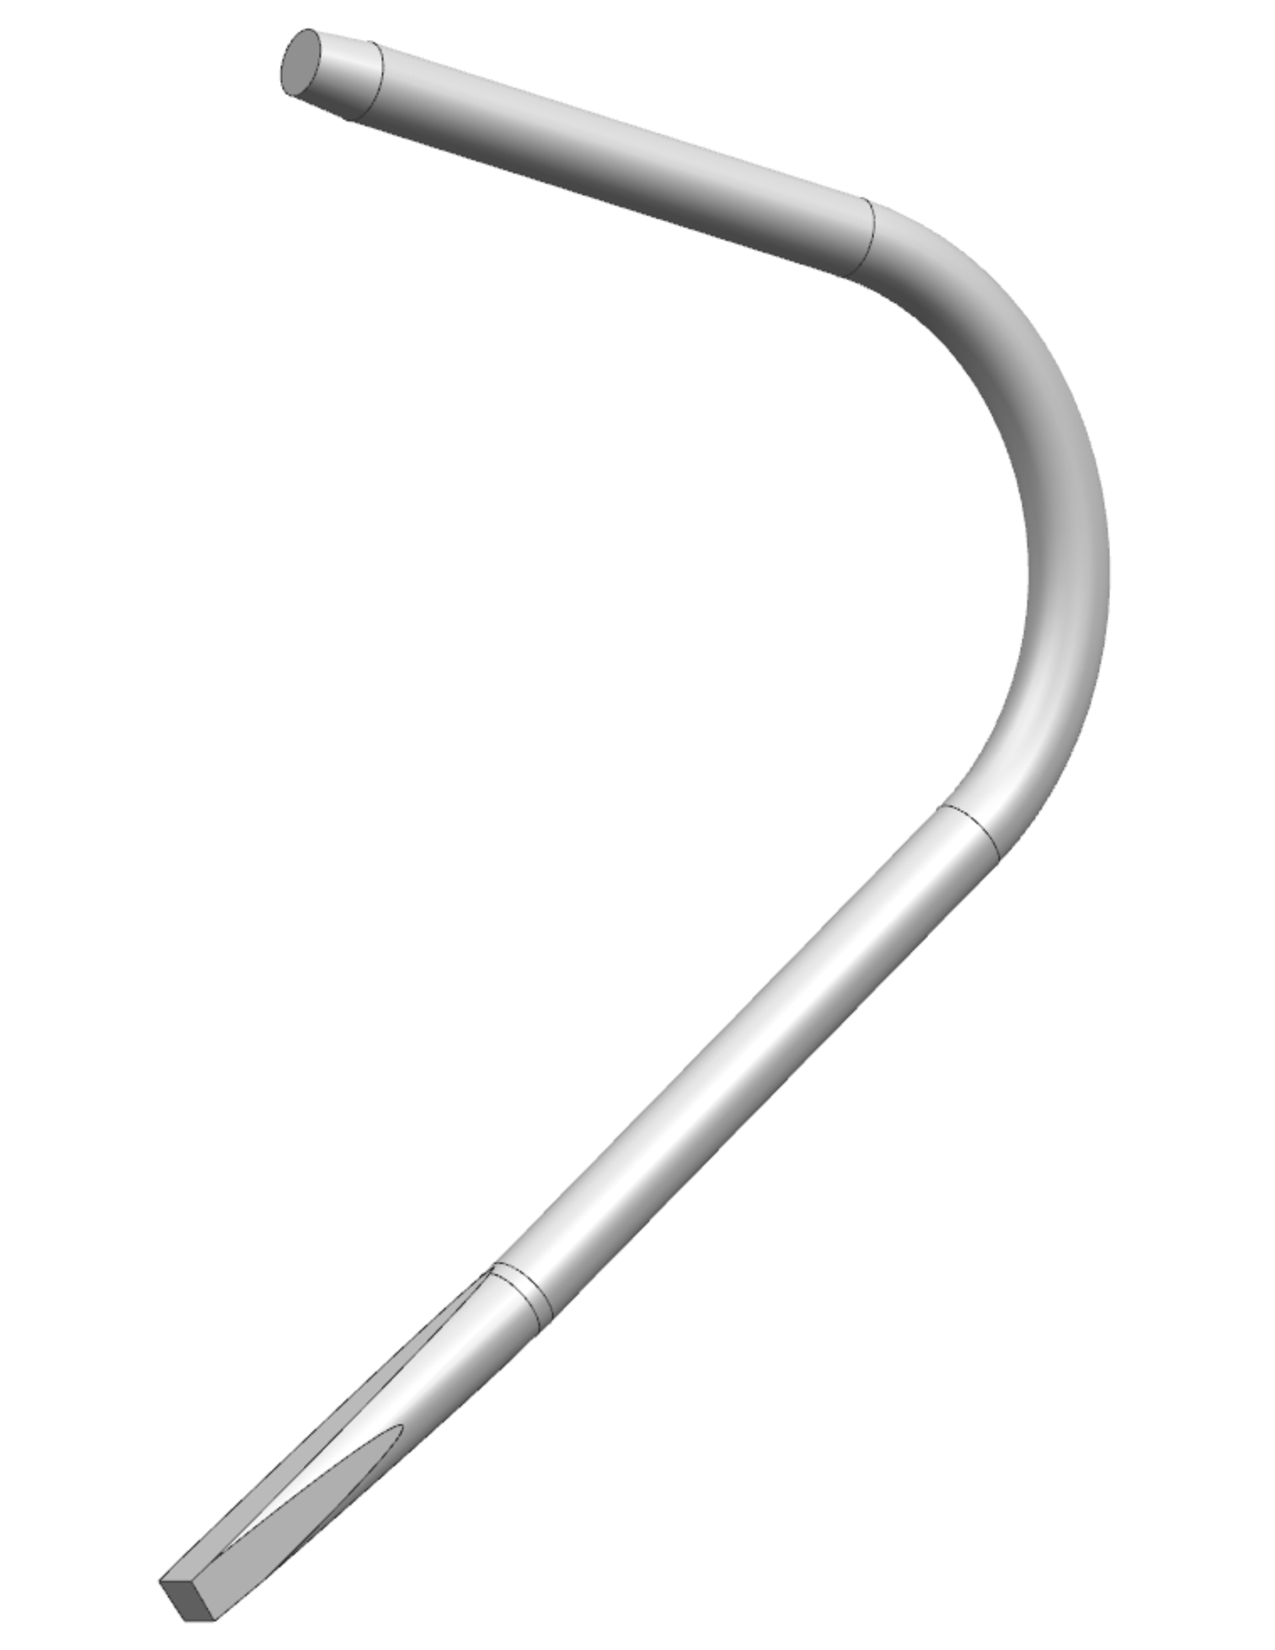
\includegraphics[width=0.40\textwidth,natwidth=610,natheight=642,angle=-80]{pics/ctof-lgd.pdf}}}
\end{picture}
\put(80,10){(a)}
\put(300,10){(b)}
\caption{The design of the CTOF (a) upstream and (b) downstream light guides. The wedge-shaped
side of each figure is the end that couples to the scintillation bar and the cylindrical side of each figure
couples to the PMT.}
\label{ctof-lg}
\end{figure}
%%%%%%%%%%%%%%%%%%%%%%%%%%%%%%%%%%%%%%%%%%%%%%%%%%%%%%%%%

The design of the upstream light guide is shown in Fig.~\ref{ctof-lg}(a). The sides of the Acrylic
cylinder were milled to a length of $\sim$25~cm along the light guide to form a wedge up to a radius
of 37~cm in the $(r,\phi)$-plane in order to fit into the $\Delta \phi=7.5^\circ$ sector. The straight
cylindrical section is $\sim$75~cm long to position the PMT in the solenoid fringe field at a position
where the maximum field is at the level of $\sim$1~kG. The design of the downstream light guide is
shown in Fig.~\ref{ctof-lg}(b). The sides of the cylinder were milled to a length of $\sim$30~cm along
the light guide to form a wedge up to a radius of 40~cm in the $(r,\phi)$ plane. The light guide bends
through an angle of 135$^\circ$ over a length of $\sim$45~cm around the downstream face of the
solenoid magnet to position the downstream PMTs in a lower maximum value of the solenoid fringe field
of about 400~G. 
 
\subsubsection{Monte Carlo Design Studies}
\label{lg-mc}

The light guide design was optimized using a Monte Carlo program to simulate light propagation
through the CTOF counter assemblies consisting of the scintillation bar, the upstream and
downstream light guides, and the PMT entry windows. The transmittance of the light guide is a
function of its material properties, such as refractive index, bulk attenuation length, and
surface reflectivity. Additionally, the light guide transmittance depends on its geometrical
shape and size. In particular, the ratio of the light guide entrance area $S_i$ to its exit
area $S_o$ is of critical importance since Liouville's phase space theorem dictates that the 
transmittance $T$ of the guiding system is constrained as:

\begin{equation}
T \le \frac{S_o}{S_i}.
\end{equation}

\noindent
Thus, in order to avoid this fundamental limitation, the PMT photocathode area $S_{pc}$ must
be larger than the area of the end of the scintillation bar. For the CTOF system we required
that $S_{pc}$ be larger than $\sim$12.5~cm$^2$. For the R2083 PMT chosen for CTOF (see
Section~\ref{PMTs}) with a 5.08-cm diameter and a 16.6~cm$^2$ photocathode area, the cross
section of the focusing light guide almost doubles from the scintillation bar end to the PMT. As
was shown through both Monte Carlo calculations and light transmission measurements
\cite{barbosa06}, this feature roughly doubles the transmittance of the focusing light guides
compared to guides of a constant cross section.

The production light guides for CTOF were therefore based on a focusing design where 
the cross section of the light guide matches to the wedge-shaped face of the scintillation bar 
and expands in cross section along its length to match the area of the PMT. The shape of such a 
light guide gradually transforms from a truncated pyramid with a trapezoidal cross section at 
the end of the scintillation bar to a cylinder in the middle part of the guide with area 
$S_c$=20.3~cm$^2$. It then maintains a constant cross section until very near the PMT location 
when it then becomes a truncated focusing cone that mates with the PMT as shown in
Fig.~\ref{ctof-lg}.

We calculated the transport efficiency of the CTOF light guides using the BARTIM code
(described in the Appendix of Ref.~\cite{mutch}) to track the photons through the system
from their generation point in the scintillation bar until they crossed a material boundary
or they interacted with a surface. At such an interface, the photon was then either totally 
internally reflected, reflected, or refracted according to the Fresnel equation. Imperfections 
on the surface of the scintillation bar or light guide were modeled by reducing the total 
internal reflection coefficient, $IR$, below 100\%. Any light that escaped from wall boundaries 
was specularly reflected with an appropriate reflection coefficient $R$. Photons that were 
absorbed were tabulated as lost. At the boundary between materials (e.g. scintillation bar - 
light guide, light guide - PMT), Snell's law was used to give the angle of the refracted 
photon. The process was repeated over thousands of photons to gain sufficient statistics to 
make design choices.

The photons generated in the scintillation bar were modeled assuming minimum-ionizing
particles normally incident on the middle of the CTOF counter. The parameters used in our 
calculations were $R$=0.9, $IR$=0.99, and a bulk attenuation length of $\lambda_p$=6.65~m 
in the Acrylic. It was assumed that the wrapping was a radiant mirror film VM-2002 from 
3M~\cite{3m-ref}. The simulation studies for the final production designs of the CTOF light
guides yielded transmittances of $\sim$60\% for the upstream light guides and $\sim$50\%
for the downstream light guides.

Each aspect of the light guide design was studied in detail to optimize its light transport 
efficiency. In the remainder of this section, some comments on different aspects of the 
design from the results of our Monte Carlo studies are highlighted.

\begin{itemize}

\item Light Guide Pitch Angles: The effect of changing the pitch angle of the upstream light 
guide from 18$^\circ$ to 30$^\circ$ was investigated. The transmission varied by less than 1\%. 
Varying the downstream pitch angle was not investigated as a different pitch angle would 
violate the defined keep-out zones of the CTOF for both the solenoid and the high-threshold 
Cherenkov detectors.

\vskip 0.5cm

\item Light Guide Length: We investigated the effect of decreasing the light guide length by 
about 250~mm. The transport efficiency of the upstream and downstream light guides improved 
by $\sim$10\% compared to our final design choice. However, the constraints on the CTOF from 
the neighboring detector subsystems and the practical design limits for the PMT magnetic 
shields, effectively set the positions of the PMTs and prevented a shorter light guide design 
from being employed.

\vskip 0.5cm

\item Extent of Wedge-Shaped Region: The transition of the light guides from the wedge-shaped 
end at the scintillation bar to the cylindrical cross section was optimized through Monte 
Carlo calculations. The design required that the light guides at the upstream and downstream 
ends of the detectors fully fit within a 7.5$^\circ$ opening from the target. The Monte Carlo 
calculations showed that the light transport efficiency is strongly dependent on the length 
of the cylindrical portion of the light guide. The longer the cylindrical portion of the light 
guide compared to the wedge-shaped region, the better the transmittance. For the upstream 
(downstream) light guides the wedge-shaped portion has an extent of $\sim$25~cm ($\sim$30~cm), 
which could not be made shorter and still have the light guide fit within its 7.5$^\circ$ 
azimuthal restriction.

\vskip 0.5cm

\item Light Guide to PMT Matching: The inner photocathode surface of the R2083 PMT used for
the CTOF readout is part of a sphere with a radius of 2.3~cm. Due to this shape, the thickness of the
entry window varies from 1~mm in the center to 7~mm at the periphery. Thus, the geometry of the
PMT entry window needs to be taken into account since photons may escape through the periphery
of the glass window, and according to our Monte Carlo simulations, the PMT window effect may
reduce the number of primary photoelectrons up to 30\%. In order to compensate for this effect,
the light guides transition from a constant cylindrical cross section to a focusing cone over their last 
$\sim$5~cm. The focusing cone slightly increases the photon angle at the exit. Simultaneously, 
the cone shrinks the luminous area and provides for slightly better targeting at the photocathode. 
Since most of the photons at the end of the cylindrical part of the light guide propagate within 
the total internal reflection angle, the focusing cone directs a substantial fraction of the 
escaping photons to the spherical photocathode. The cone length and opening angle were optimized 
for the best possible transmittance. 

\end{itemize}

\subsubsection{Optical Tests of Acrylic}
\label{optical-tests}
  
In order to evaluate the optical properties of the Acrylic light guides in terms of light
transmittance, we developed a technique for rapid measurements using the setup shown in 
Fig.~\ref{trans-setup}. We define the light transmittance of our light guides as the ratio 
of the light guide output radiation to input radiation. For our measurements we injected 
diffuse light of $\sim$450~nm wavelength into the light guide along its axis from one end. 
At the opposite end we mounted an ILT1400 radiometer~\cite{ilt-ref}, which functioned as a
photodetector. In order to determine the transmittance $T$ we compared two measurements
of the transmitted radiation $R$. The first value was measured with a very short reference
light guide and the second value was measured with the light guide under study. This method
automatically compensated for apparent light losses due to surface reflections. The transmittance
of the light guide was computed as:  

\begin{equation}
\label{trans}
T = \frac{R(l_x)}{R(l_s)},
\end{equation}

\noindent
where $l_x$ is the length of the light guide (1~m upstream, 1.6~m downstream), $l_s$ is the length
of the short rod (2.5~cm), and $R(l)$ is the transmitted light intensity measured with the sample of
length $l$. 

%%%%%%%%%%%%%%%%%%%%%%%%%%%%%%%%%%%%%%%%%%%%%%%%%%%%%%%%%
\begin{figure}[htbp]
\vspace{2.5cm}
\begin{picture}(50,50) 
\put(95,-70)
{\hbox{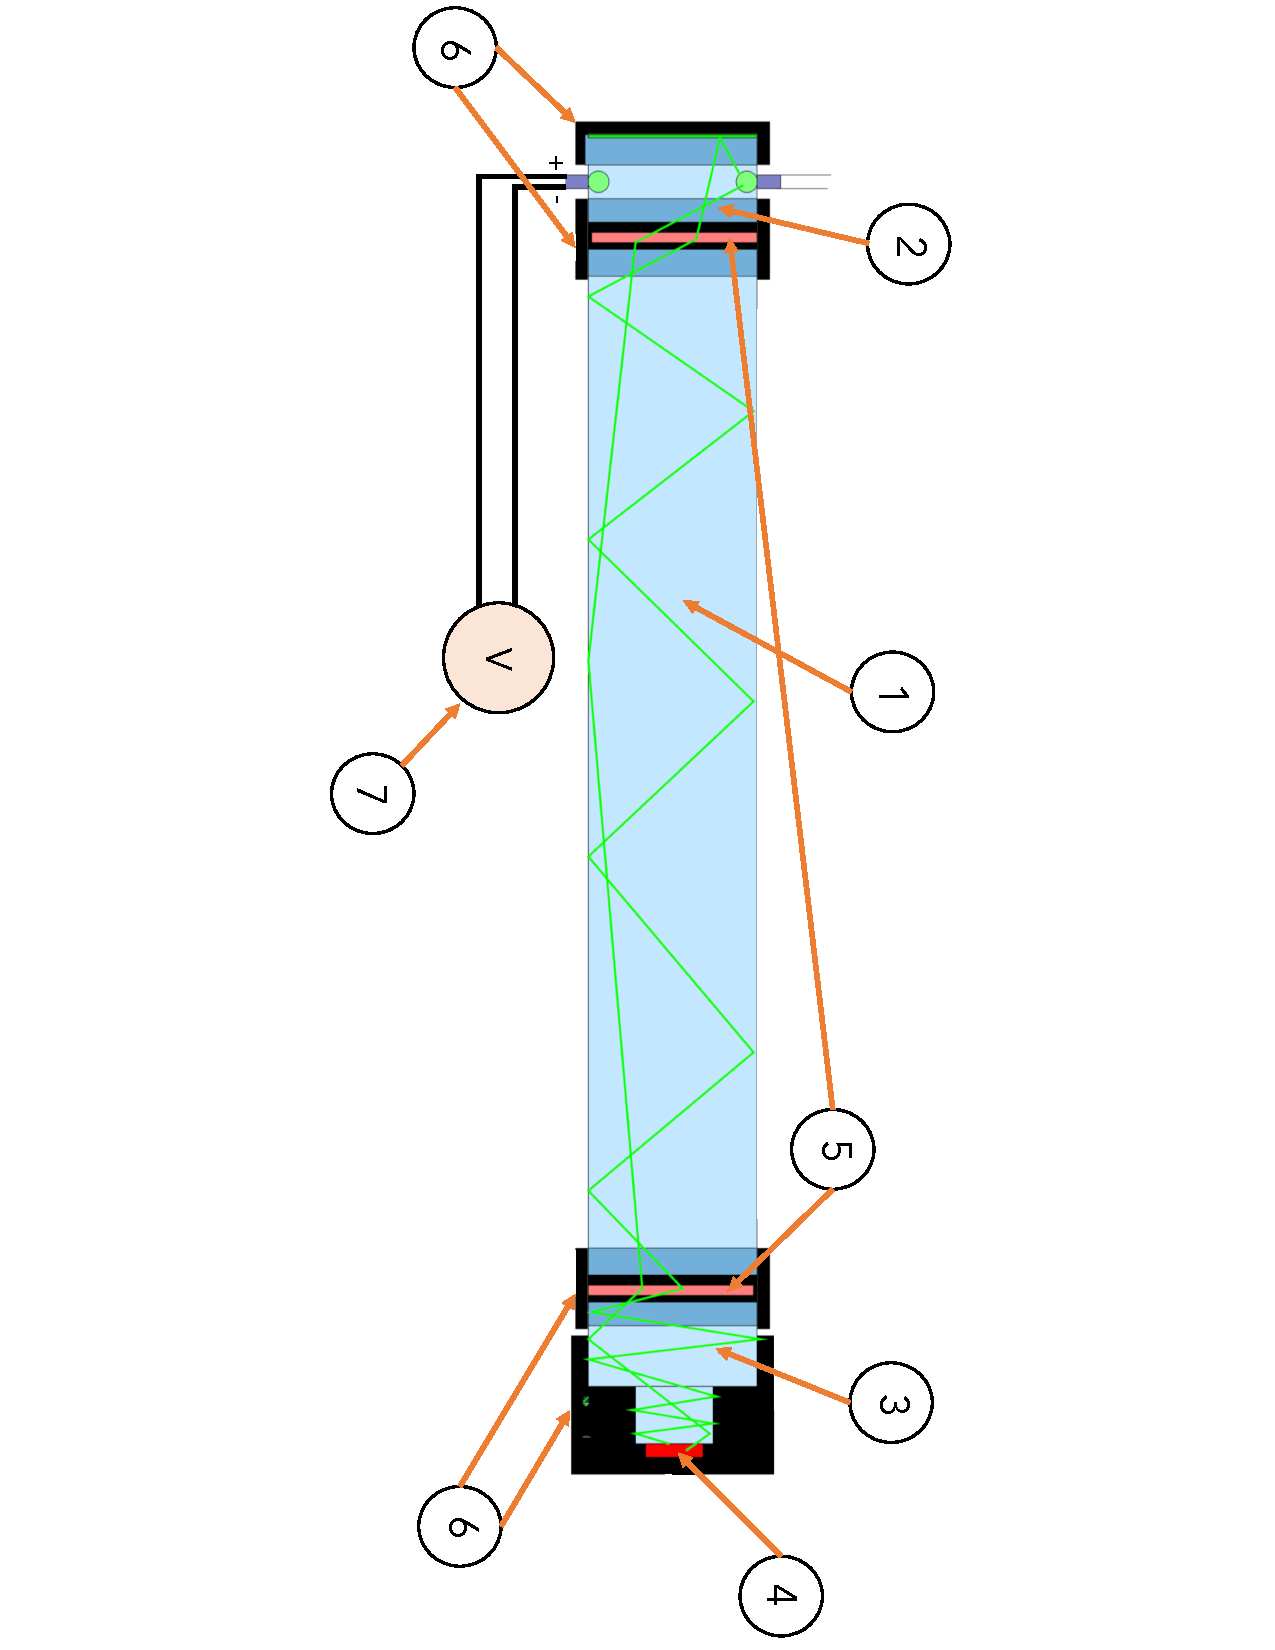
\includegraphics[width=0.65\textwidth,natwidth=610,natheight=642,angle=90]{pics/lg-trans-setup.pdf}}}
\end{picture} 
\caption{(Color Online) CTOF setup for the light guide transmittance measurements. (1) Acrylic rod,
(2) light source, (3) Acrylic piece, (4) silicon photodetector, (5) Teflon film as a diffuser, (6) mount units,
and (7) digital voltmeter.}
\label{trans-setup}
\end{figure}
%%%%%%%%%%%%%%%%%%%%%%%%%%%%%%%%%%%%%%%%%%%%%%%%%%%%%%%%%

From these data for our upstream (downstream) light guides, we measured an average
transmittance of $\sim$60\% ($\sim$50\%). Studies of our test setup indicated that our 
transmittance measurements were accurate to the few percent level. These values can be 
compared directly to measurements of the photoelectron statistics using cosmic ray data for a
configuration with a CTOF scintillation bar coupled directly to a PMT to that where the
scintillation bar is coupled to a production CTOF light guide. Our findings showed that the ratio
of photoelectrons was $\sim60\pm5$\% and $\sim50\pm5$\% for the upstream and downstream
light guides, respectively, in agreement with our bench measurements and our Monte Carlo
calculation results discussed in Section~\ref{lg-mc}.

From the transmittance data the practical attenuation length (see Section~\ref{scint-mat} 
for a discussion of practical vs. bulk attenuation lengths) of the light guide can be defined as:

\begin{equation}
\label{pracat}
\lambda= \frac{(l_s-l_x)}{\ln(T)},
\end{equation}

\noindent
which assumes an exponential attenuation of light along the light guide. The average practical 
attenuation length measured for the CTOF Acrylic light guides was $\sim$2.3~m.

In order to characterize the bulk attenuation length of our chosen Acrylic material, the
same measurement system shown in Fig.~\ref{trans-setup} was employed. For these measurements 
the Teflon film light diffuser was removed. For this case the sensor area of the photometer 
($\sim$1~cm$^2$) was large enough to intercept the full transmitted beam. The average bulk 
attenuation length of the Acrylic material was measured to be 6.65$\pm$0.5~m.

\subsection{Photomultiplier Tube/Voltage Divider Assemblies} 
\label{PMTs}

The selection of the PMTs for the CTOF detector considered a number of different solutions,
including both conventional PMTs and field-resistant PMTs. Our final choice, which was 
thought to be the most conservative design, opted for conventional PMTs contained within a
magnetic shield system at the ends of long light guides to position the PMTs well outside of
the extremely high field region of the solenoid magnet.

Our studies showed that the optimal light guide design should have an increasing cross
section from the scintillation bar to the PMT to optimize the light transmission efficiency.
Given the average surface area of the end face of the scintillation bars of 11.45~cm$^2$, we 
selected a 5.08-cm diameter PMT for the readout. This corresponds to a surface area of 
20.0~cm$^2$. The size matching comparison is shown in Fig.~\ref{matching}. Our choice for the 
CTOF readout was the H2431 PMT/voltage divider assembly from Hamamatsu~\cite{ham-ref}.
This integrated assembly employs the 5.08-cm diameter Hamamatsu R2083 PMT~\cite{r2083-ref}.
The relevant specifications for this PMT are listed in Table~\ref{pmt-specs}. Fig.~\ref{H2431}
shows a schematic of the H2431 assembly and the circuit diagram for the voltage divider.

For the R2083 PMT the diameter of the photocathode is 46~mm. As with most timing PMTs, it
has a spherical photocathode. Such a shape is helpful to equalize path lengths of the primary 
photoelectrons to the first dynode. However, due to this spherical shape, the accelerating electric
field always has a component perpendicular to an axial magnetic field. Therefore timing PMTs like
the R2083 are sensitive to the axial components of the magnetic fringe field. The expectation for
these PMTs is that they can operate in an environment such that the maximum allowable axial field
at the photocathode is 0.4~G. However, we have aimed to achieve fields of $\le$0.2~G at the 
photocathode to maintain a reasonable safety margin.

%%%%%%%%%%%%%%%%%%%%%%%%%%%%%%%%%%%%%%%%%%%%%%%%%%%%%%%%%
\begin{table}[htbp]
\begin{center}
\begin{tabular}{ll} \hline
Spectral response           & 300 $\to$ 650~nm \\
Wavelength of max. emission & 420~nm \\
Photocathode material       & Bialkali \\
Minimum effective area      & 46~mm \\
Window material             & Borosilicate glass \\
Dynode                      & 8 stage, linear focused \\
Gain                        & 2.5$\times$10$^6$ \\
Quantum Efficiency @ $\lambda_{max}$ & 27\% \\
Max. anode current rating   & 200~$\mu$A \\
Anode dark current (typical) & 100~nA \\
Anode pulse rise time       & 0.7 ns \\
Electron transit time       & 16 ns \\
Transition time spread      & 0.37 ns \\ \hline
\end{tabular}
\end{center}
\caption{The properties of the Hamamatsu R2083 PMT used for the CTOF readout.}
\label{pmt-specs}
\end{table}
%%%%%%%%%%%%%%%%%%%%%%%%%%%%%%%%%%%%%%%%%%%%%%%%%%%%%%%%%

%%%%%%%%%%%%%%%%%%%%%%%%%%%%%%%%%%%%%%%%%%%%%%%%%%%%%%%%%
\begin{figure}[htbp]
\vspace{3.8cm}
\begin{picture}(50,50) 
\put(150,130)
{\hbox{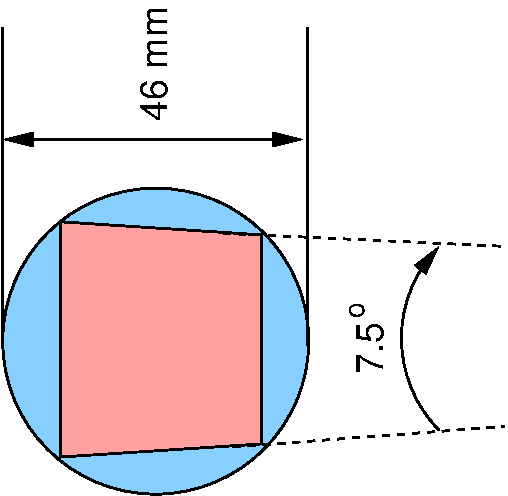
\includegraphics[width=0.80\textwidth,natwidth=610,natheight=642,angle=-90]{pics/inscribe1.pdf}}}
\end{picture} 
\caption{(Color Online) The cross section of the end face of the scintillation bar (wedge cross section)
inscribed into the photocathode of the R2083 PMT (circular cross section). The light guides match the
shape of the scintillation bar on one end and the shape of the PMT on the other.}
\label{matching}
\end{figure}
%%%%%%%%%%%%%%%%%%%%%%%%%%%%%%%%%%%%%%%%%%%%%%%%%%%%%%%%%

%%%%%%%%%%%%%%%%%%%%%%%%%%%%%%%%%%%%%%%%%%%%%%%%%%%%%%%%%
\begin{figure}[htbp]
\vspace{10.0cm}
\begin{picture}(50,50) 
\put(-15,340)
{\hbox{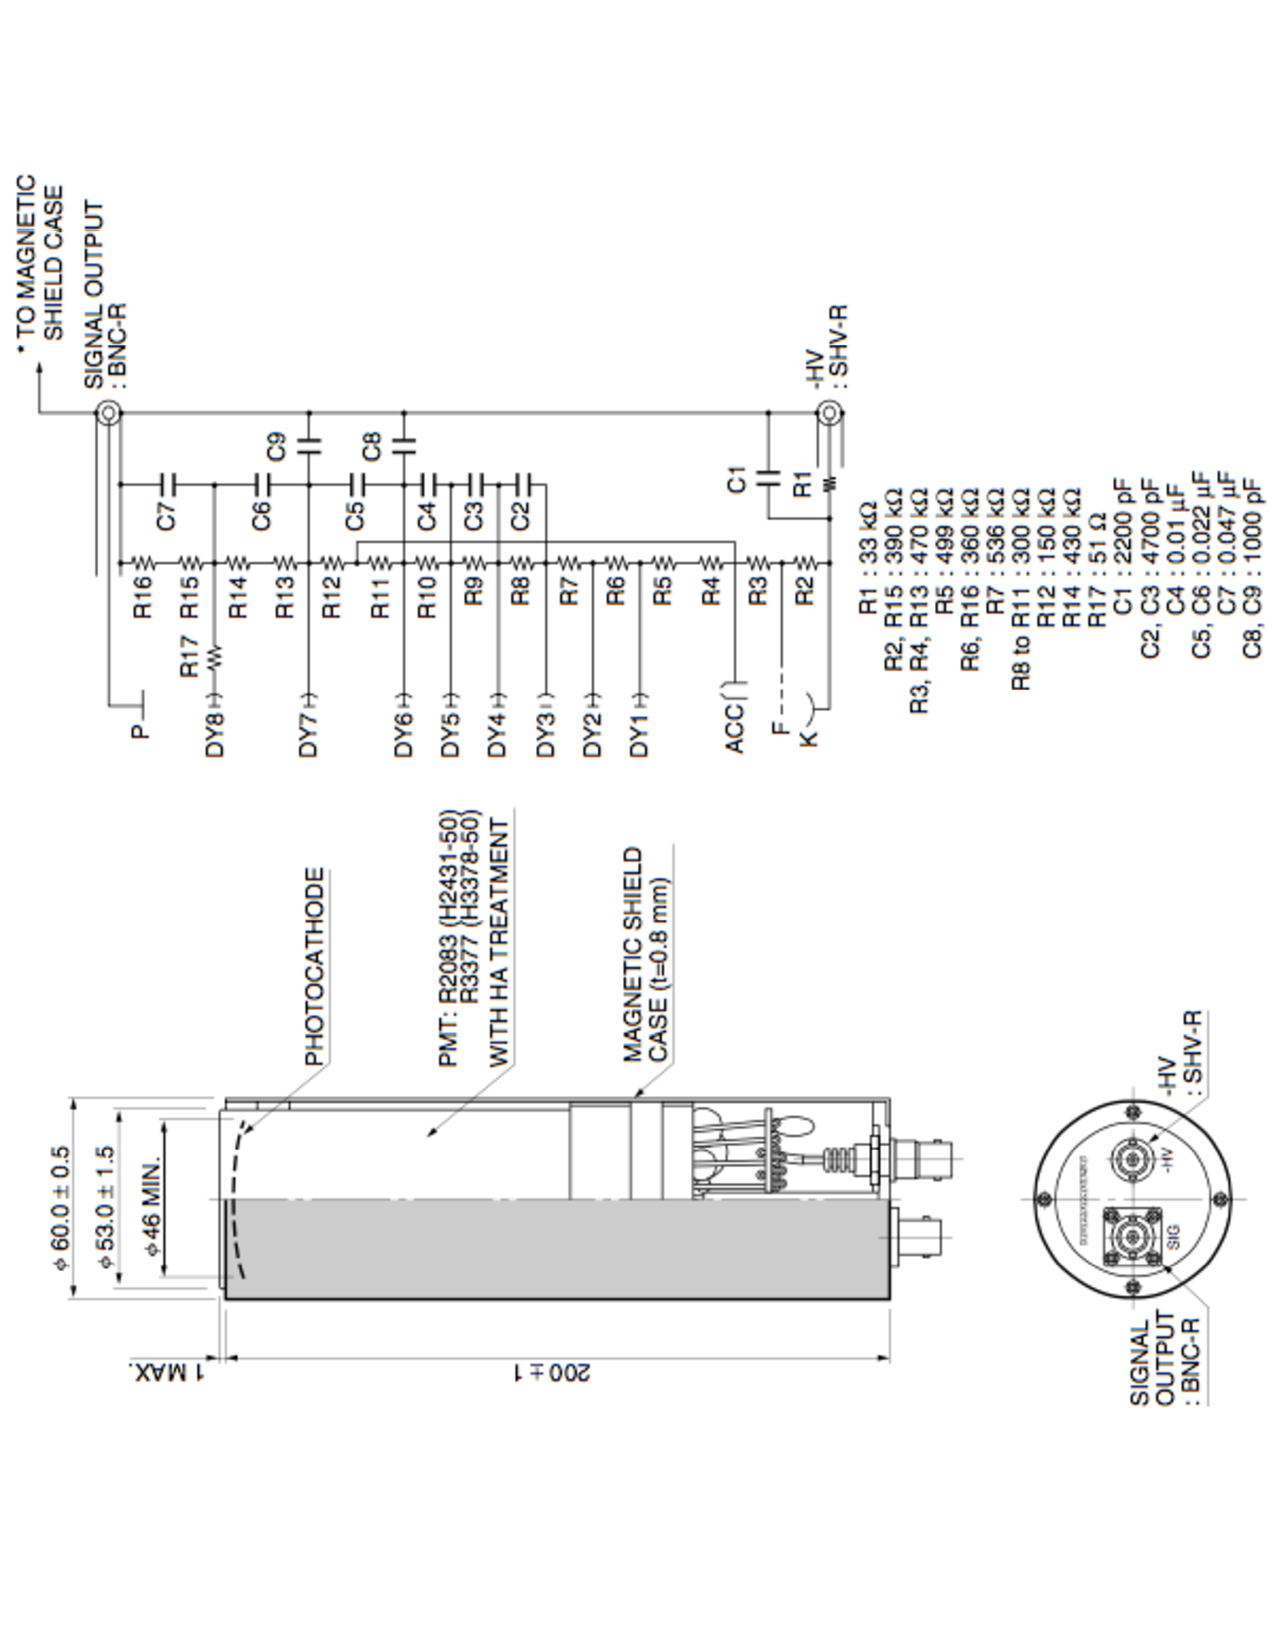
\includegraphics[angle=-90,width=0.90\textwidth,natwidth=610,natheight=642]{pics/h2431.pdf}}}
\end{picture} 
\caption{Schematic diagram of the Hamamatsu H2431 assembly based on the R2083 5.08-cm diameter
PMT used for the CTOF readout~\cite{ham-schem}. Note that for this application the supplied magnetic
shield case was not used.}
\label{H2431}
\end{figure}
%%%%%%%%%%%%%%%%%%%%%%%%%%%%%%%%%%%%%%%%%%%%%%%%%%%%%%%%%

Alternative solutions for the PMTs were considered, specifically in terms of field-immune and
field-resistant devices. If such PMTs could be used (and were competitive in terms of pricing
compared to conventional PMTs), then the CTOF could have been designed without the need for long
light guides or possibly without any light guides whatsoever. One solution considered employed 
the Burle 85011 micro-channel plate (MCP) PMT~\cite{burle-ref}. These devices have immunity to
magnetic fields up to $\sim$2~T, while providing very good timing resolution~\cite{kichimi}.
However, the drawback of MCP PMTs is that their quantum efficiency (QE) is only about half that
of conventional PMTs, which would have an adverse affect on the counter timing resolution that has
the behavior,

\begin{equation}
\sigma_{PMT} \propto \frac{1}{\sqrt{N_{ph} \cdot QE}},
\end{equation}

\noindent
where $N_{ph}$ is the number of incident photons at the photocathode of the PMT. From our studies
the choice of a conventional PMT with a long light guide compared to an MCP PMT with no light guide
gave comparable resolutions~\cite{baturin06}.

The issue of low QE of the MCP PMT can be solved with fine-mesh (FM) PMTs, which have been
shown to operate in fields up to 1~T, or metal-channel (MC) PMTs, which hold promise of
operating well in fields up to 0.2~T. With either the FM or MC PMTs as solutions for the CTOF,
shorter light guides could be employed in the design.

Several different FM PMTs were studied during the CTOF design phase, including the R5505,
R7761, and R5924 from Hamamatsu. These FM PMTs were shown to have stable timing response
in external fields up to 1.2~T~\cite{bonesini}. The R5924 with photocathode size of 39~mm
and the R7761 with photocathode size of 27~mm were poor matches to our required light guide
dimensions. The R6504 with photocathode area of 51~mm, which has a dimension directly comparable
to the R2083, however, was discontinued by Hamamatsu. In our studies that directly compared
the intrinsic time resolution of the R2083 to the R5924 using an LED source with each PMT
seeing exactly the same amount of light, the resolution of the R5924 was found to be roughly 
a factor of two worse than the R2083. These findings were confirmed in beam studies in
Hall~B at JLab~\cite{baturin11}.

We also considered MC PMTs such as the H8500 and R7400 from Hamamatsu. These devices have
excellent timing characteristics (with a transition time spread $\sigma_{TTS}$=400~ps), 
comparable QE to conventional PMTs, and have been shown to be able to operate in external 
fields up to 0.2~T. The technical issue with the MC PMT is that its intrinsic gain is 
roughly a factor of three smaller than for the R2083 and signal to noise ratio concerns 
become an issue.

\subsubsection{Rate-Stabilized Divider}
\label{divider}

The voltage divider circuit shown in Fig.~\ref{H2431} is a standard inclusion with the
R2083 PMT in the Hamamatsu H2431 assembly. Due to the requirement of stable PMT performance
in terms of gain and timing response in the high rate environment of the CTOF detector
just outside of the beam-target interaction region, we have made a small modification to
the stock Hamamatsu divider to improve its stability to higher currents. A small amplifier 
circuit has been inserted as a sequential component after the last resistor in the divider. 
This active division circuit consists of two transistors that are powered by the current 
flowing through the divider. A version of this circuit design is described in Ref.~\cite{popov}. 

%%%%%%%%%%%%%%%%%%%%%%%%%%%%%%%%%%%%%%%%%%%%%%%%%%%%%%%%%
\begin{figure}[htbp]
\vspace{3.0cm}
\begin{picture}(50,50) 
\put(0,-155)
{\hbox{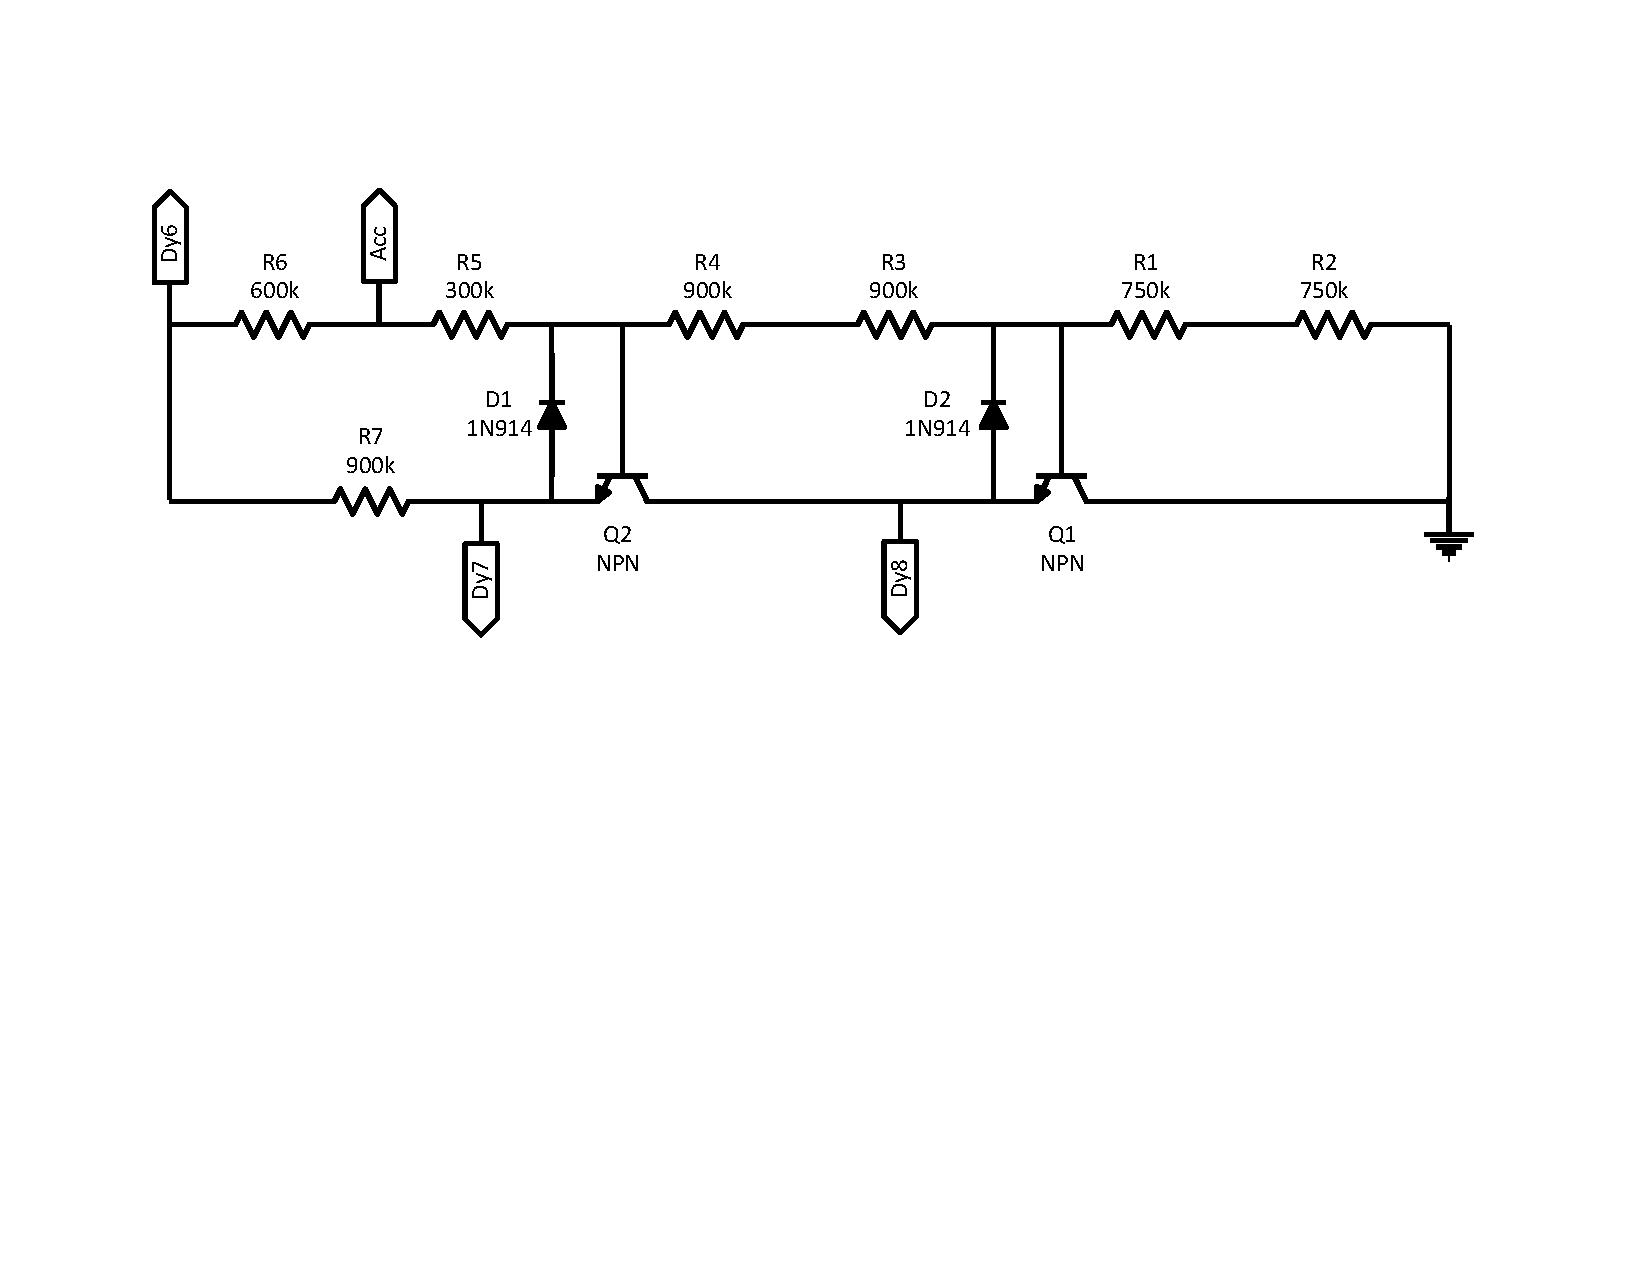
\includegraphics[width=0.80\textwidth,natwidth=610,natheight=642]{pics/amp-circuit.pdf}}}
\end{picture} 
\caption{Schematic diagram of the JLab-designed transistorized impedance matching amplifier 
circuit added to the standard Hamamatsu R2083 voltage divider.}
\label{popov-mod}
\end{figure}
%%%%%%%%%%%%%%%%%%%%%%%%%%%%%%%%%%%%%%%%%%%%%%%%%%%%%%%%%

The active divider circuit is an amplifier that is actually an impedance converter, which 
provides an output impedance termination matching to a standard 50~$\Omega$ coaxial cable.
The active divider circuit is mounted on a small mezzanine board that is soldered into the 
stock R2083 divider. It is connected to Dy6, Dy7, Dy8, ACC (see Fig.~\ref{H2431}), and 
grounded as shown in the circuit schematic of Fig.~\ref{popov-mod}. The passive divider 
resistors connected to those dynodes were removed and all capacitors were left in place. The 
transistors employed are high voltage (400~V or better rated) Si NPN types. 

Fig.~\ref{mod-div-plots} compares the performance of the stock R2083 voltage divider from
Hamamatsu to that of a typical modified divider. This figure shows a comparison of the gain 
stability of the PMT/divider assemblies as a function of the PMT anode current. The gain of the 
modified divider is seen to be more independent of current up to 200~$\mu$A, the maximum 
rated current of the device, compared to the stock divider. Fig.~\ref{mod-div-plots} also 
shows a corresponding improvement in the stability of the timing response up to 200~$\mu$A.

%%%%%%%%%%%%%%%%%%%%%%%%%%%%%%%%%%%%%%%%%%%%%%%%%%%%%%%%%
\begin{figure}[htbp]
\vspace{7.7cm}
\begin{picture}(50,50) 
\put(55,-75)
{\hbox{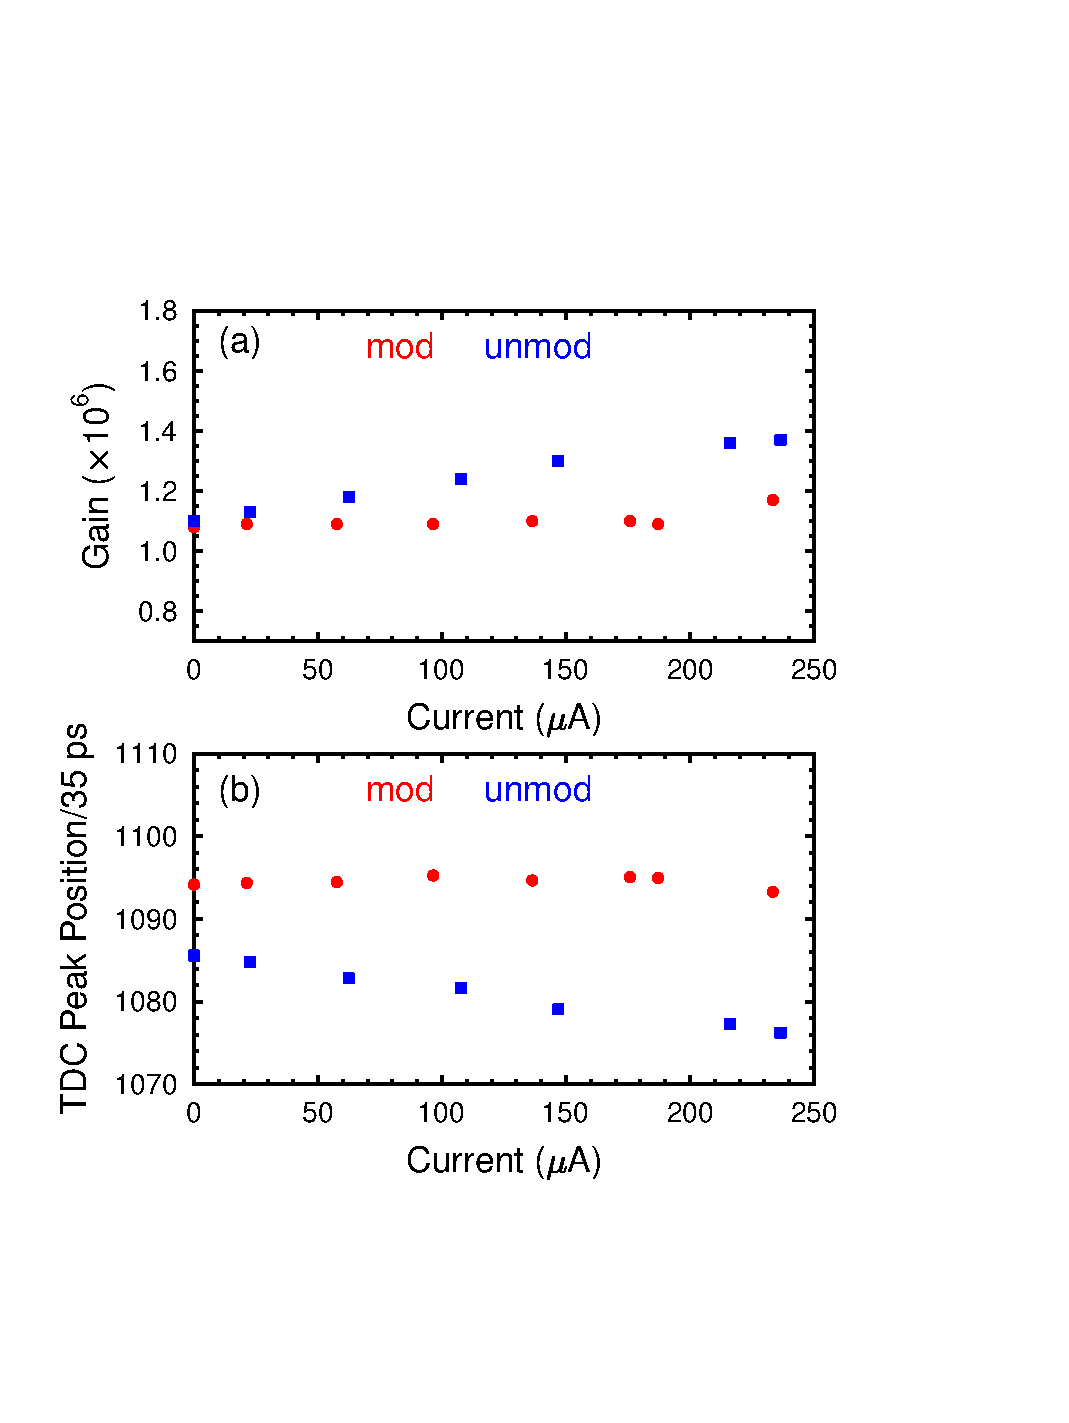
\includegraphics[width=0.95\textwidth,natwidth=610,natheight=642]{pics/divider.pdf}}}
\end{picture} 
\caption{(Color Online) Comparison of the performance of the R2083 PMT vs. PMT anode current
($\mu$A) with its stock divider (blue squares) compared to that of an R2083 PMT with the modified
divider (red circles) showing (a) the gain stability and (b) the timing response stability.}
\label{mod-div-plots}
\end{figure}
%%%%%%%%%%%%%%%%%%%%%%%%%%%%%%%%%%%%%%%%%%%%%%%%%%%%%%%%%

\subsection{Magnetic Shields}
\label{sec:shields}

\subsubsection{CLAS12 Solenoid Field}

The CLAS12 solenoid is a self-shielded superconducting magnet that is used to produce a field 
primarily along the beam direction about the target. The magnet has an inner diameter of 100~cm 
and is roughly 1.5~m long. The central field of the magnet is 5~T at its nominal full current. 
Outside the magnet a sizable fringe field extends for several meters in all directions. Given 
the many design constraints for the CLAS12 Central Detector region that essentially localized 
the positions of the CTOF counter elements, the PMTs are located in fringe fields from the 
solenoid at levels up to $\sim$1~kG.

To determine the necessary shield reduction factors at the locations of the PMTs, the field
values at the locations of one upstream high-pitch angle and one low-pitch angle PMT were
determined using a map of the CLAS12 solenoid fringe field was based on a full 3-D 
finite-element analysis calculation using the OPERA-TOSCA suite~\cite{opera} to model the 
magnet. Note that due to the azimuthal symmetry of the solenoid fringe field, the field 
strengths and gradients at the locations of the full set of CTOF upstream PMTs can be assumed 
to be the same. Table~\ref{field-position} provides the field components of the CLAS12 
solenoid fringe field at the locations along the axis of the PMT at the photocathode (i.e. 
the face of the PMT), the first dynode (a distance 3~cm from the photocathode), and the middle 
of the accelerating structure (a distance 5.5~cm from the photocathode) for both PMTs. All of 
the fields are necessarily given without any shields present as the shields strongly modify the 
local fringe field distributions. Table~\ref{field-position} also includes the field components 
along the PMT axes at the locations of the end faces of the shield assemblies. Shield end \#1 
is the end closest to the magnet and shield end \#2 is the end farthest from the magnet. For 
shield end \#1, the strength of the field for the high-pitch angle design is 1000~G and for the 
low-pitch angle design is 1076~G. However, due to the different positions of these shields in 
the solenoid fringe field, the corresponding axial and transverse field components at these 
locations for the two designs are significantly different.

%%%%%%%%%%%%%%%%%%%%%%%%%%%%%%%%%%%%%%%%%%%%%%%%%%%%%%%%%
\begin{table}[htbp]
\begin{center}
\begin{tabular} {|c|c|c|} \hline
               & High-Pitch Angle & Low-Pitch Angle \\ \hline
Position       & $(B_y,B_z)$      & $(B_y,B_z)$  \\ \hline
Shield End \#1 & (981, 192) G     & (956, 493) G \\ \hline
Photocathode   & (612, 118) G     & (632, 329) G \\ \hline
First Dynode   & (491,  93) G     & (490,  27) G \\ \hline
Middle Dynode  & (405,  85) G     & (416, 221) G \\ \hline
Shield End \#2 & (337,  78) G     & (342, 193) G \\ \hline \hline
\end{tabular}
\end{center}
\caption{Magnetic field components along the central axis of a representative upstream CTOF 
PMT of the high-pitch angle and the low-pitch angle designs positioned in the $(y,z)$ plane 
in the CLAS12 coordinate system ($y$-axis points up, $z$-axis is along the beamline). The
associated field components are from a 3-D field map of the CLAS12 solenoid. The positions are
locations along the associated PMT axes at the photocathode, the first dynode, the middle of the
accelerating structure, and at the end faces of the magnetic shield volumes.}
\label{field-position}
\end{table}
%%%%%%%%%%%%%%%%%%%%%%%%%%%%%%%%%%%%%%%%%%%%%%%%%%%%%%%%%

For the positioning of the CTOF magnetic shields in the CLAS12 solenoid fringe field, the field 
lines are at roughly 40$^\circ$ with respect to the axis of the PMT. In this case roughly two-thirds
of the field is axial, which produces a smaller effect on PMT performance than the transverse
component, but is more difficult to shield.

We do not consider here the PMTs at the downstream end of the magnet. However, using the field 
map and the known downstream PMT locations, the maximum field strength for the downstream PMTs 
within the shield volume is $\sim$400~G. Because we have opted to use an identical shield for all
CTOF PMTs, the discussion here focuses only on the shield design for the upstream PMTs. A shield
designed for the fields seen at the upstream PMT locations will necessarily work to shield the lower
field seen at the downstream PMT locations.

\subsubsection{Shield Design}

The timing performance of PMTs in external magnetic fields deteriorates due to the Lorentz 
force. After an external photon hits the surface of the photocathode and knocks out a primary 
photoelectron, the electron accelerates toward the first dynode along the electric field lines. 
In most timing PMTs, the photocathode is shaped as a segment of a sphere. The first dynode is 
located close to the center of this sphere where the electric field lines concentrate. This 
design provides for equal travel times for the electrons created at different parts of the 
photocathode. However, even an axial magnetic field has a transverse component to the electric 
field, and Lorentz forces affect both the propagation time and the destination of the electrons, 
depending on the design of the accelerating electrode. In designing magnetic shields for the CTOF 
PMTs, we have been careful to consider both axial and transverse magnetic field components.

Various multi-layer shield designs for the CTOF PMTs were studied that were comprised of different
coaxial ferromagnetic cylinders. Ultimately we found that a 28-cm-long, three-layer shield
composed of 1008 steel of maximum thickness of 1.7~cm for the outer layer, a 3-mm-thick layer 
of the ferromagnetic HiPerm-49 for the middle layer, and a 0.8-mm-thick layer of the 
ferromagnetic Co-NETIC for the inner layer, provided the best performance within the CTOF 
magnetic field environment. Modeling calculations and measurements with physical prototypes 
showed that such a shield design can reduce a 1~kG external axial field to the level of 
$\sim$0.5~G at the location of the PMT. To reduce the remaining remnant field to the level 
of $\sim$0.2~G, a compensation solenoid coil is included just outside of the inner 
ferromagnetic layer. The design of the magnetic shield system for the CTOF PMTs is discussed 
in Refs.~\cite{baturin12,cn2015-003}.

In order to make the magnetization more uniform across the outer shielding cylinder, an 
improved design has been realized by using a tapered cylinder 1.0~cm thick at the ends and 
1.7~cm thick in the middle.  Since both the magnetic field flux and the material thickness 
increase linearly toward the middle of the cylinder, the magnetic field density in the shield 
layer is almost constant. This maximizes the permeability and results in significantly lower 
and more uniform fields inside the cylinder, which improves the shielding capability of the 
inner layers.

Ferromagnetic materials for shielding applications are of two types, those with high saturation
and those with high permeability. In very high fields, materials with high saturation should
be used. This is the reason why we chose 1008 steel for our outermost shield layer. In
moderate fields, ferromagnetics with high permeability can be used. The alloy HiPerm-49
(48\% Ni, 0.5\% Mg, 0.35\% Si, 0.02\% C, balance Fe) was chosen, which has a saturation flux 
density of $\sim$1.5~T after hydrogen annealing. Thin cylinders made of high permeability 
materials are useful in small magnetic fields. For the inner shield layer Co-NETIC was selected, 
an alloy that contains 80.6\% Ni and 14\% Fe, which saturates at about 0.8~T and is in the same 
family metallurgically as $\mu$-metal.

Using coaxial cylinders meets the design requirement that the magnetic shields have openings 
for the coaxial light guides. Therefore, axial field lines can easily penetrate inside the 
shield. In order to eliminate this effect, an approach has been developed using a 
combination of passive and active elements. In this design, the compensating solenoid that 
makes up the active element controls the magnetization of the ferromagnetic layers, including 
the innermost shield layer, which determines the field within the PMT (see 
Section~\ref{comp-coils}).

Fig.~\ref{bshield-3d} shows a cut-away view of the CTOF PMT shield system from our 3-D design 
model to highlight the components that make up the different layers and their positioning with 
respect to each other. The inner shield layers are attached to the light guide using a 
supporting clamp and the steel shield layer is attached to a support structure secured to the 
CLAS12 solenoid. Note that both the external and the intermediate shield layers actually 
consist of a cylindrical section with conical endcaps that fit tightly together. The conical 
endcaps help to capture more field lines at low radial coordinates compared to a flat cylinder. 
This feature results in a lower inner field with better uniformity along the central axis. The 
PMT itself fits within the inner shield cylinder and the light guide feeds into the opening on 
the downstream end of the shield assembly. The full weight of each shield assembly is 
$\sim$40~lbs.

%%%%%%%%%%%%%%%%%%%%%%%%%%%%%%%%%%%%%%%%%%%%%%%%%%%%%%%%%
\begin{figure}[htbp]
\vspace{2.3cm}
\begin{picture}(50,50) 
\put(25,185)
{\hbox{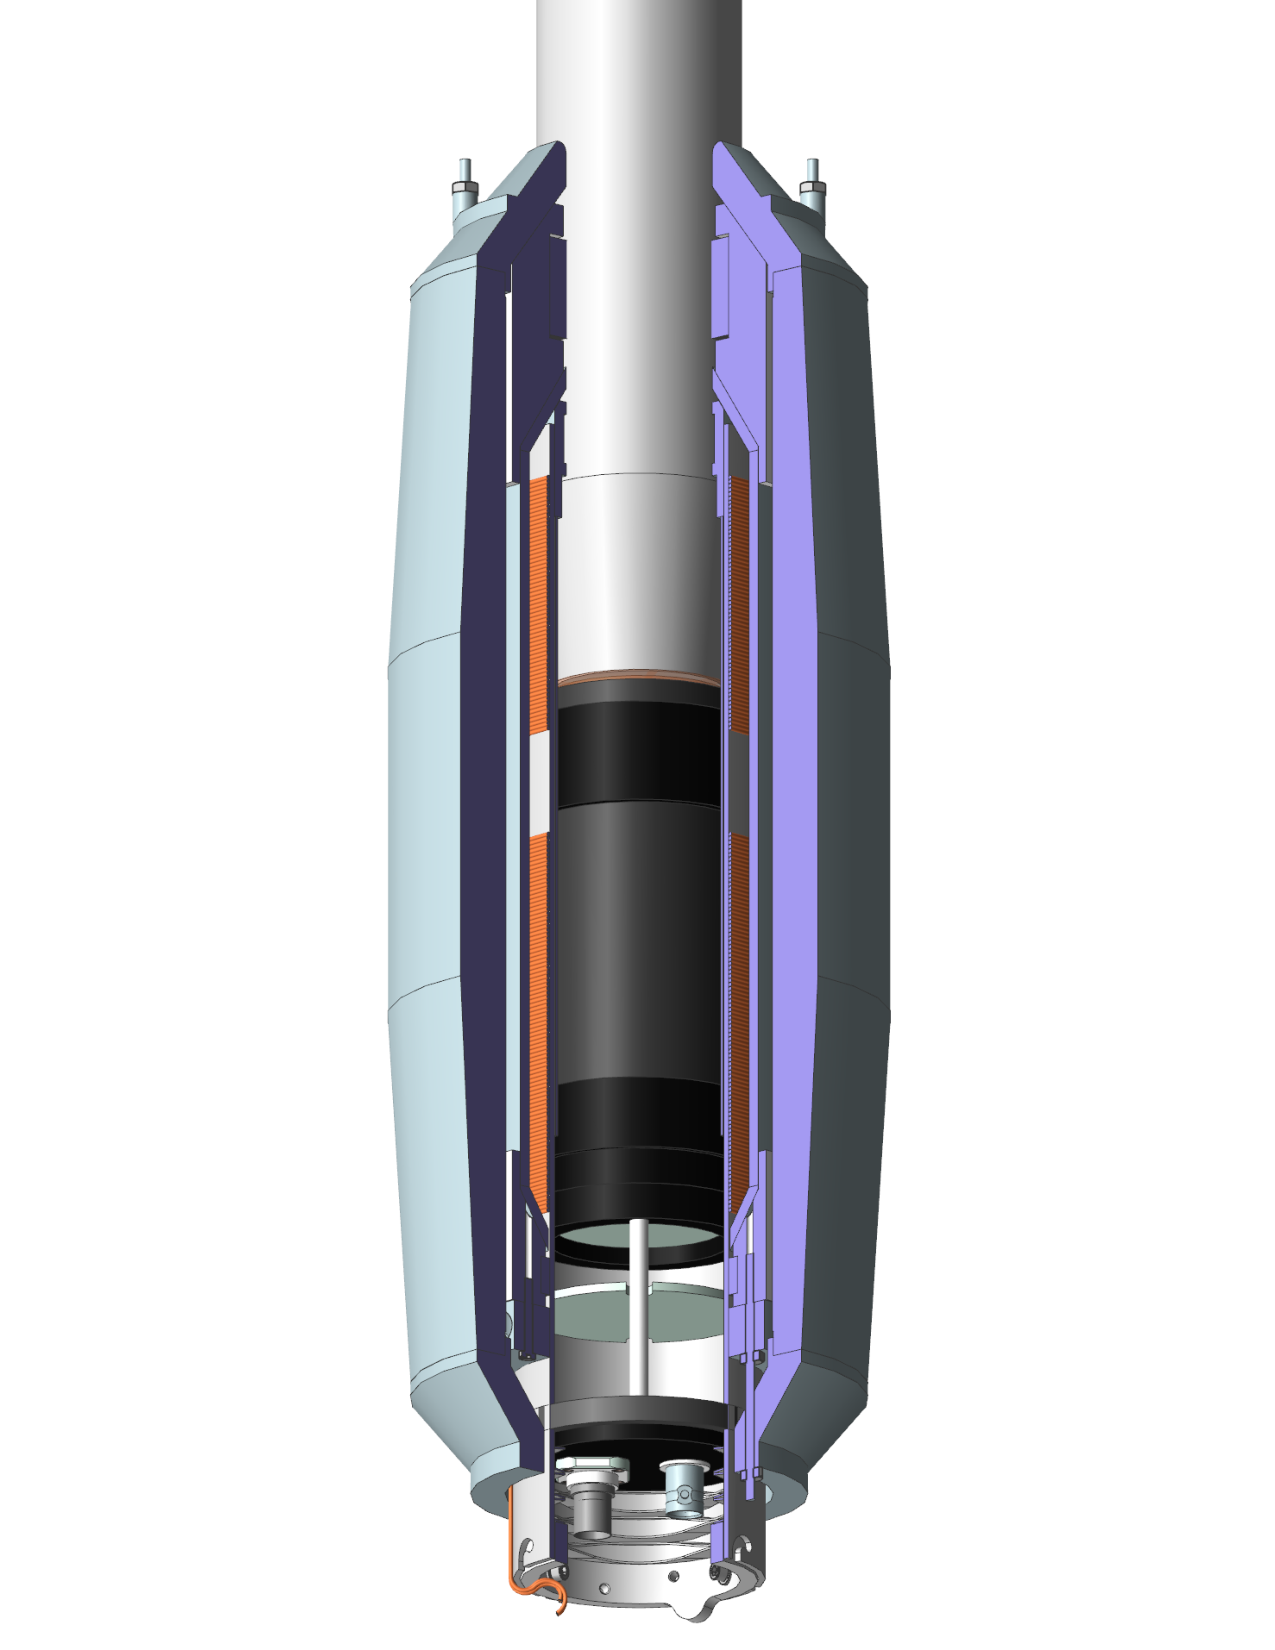
\includegraphics[angle=-90,width=0.70\textwidth,natwidth=610,natheight=642]{pics/bshield.pdf}}}
\end{picture} 
\caption{(Color Online) The CTOF shield as shown in a 3-D cut-away view. The black cylinder in the
middle of the shield is the PMT. The light guide enters the shield from the right-hand side. The two 
orange bands outside the PMT are the compensation coils.}
\label{bshield-3d}
\end{figure}
%%%%%%%%%%%%%%%%%%%%%%%%%%%%%%%%%%%%%%%%%%%%%%%%%%%%%%%%%

\subsubsection{Compensation Coils}
\label{comp-coils}

A compensation coil of 150 turns of 1-mm-thick magnet wire (18~AWG copper with a polyurethane 
and polyimide overcoat) was wound on an aluminum mandrel that was positioned between the 
inner and middle ferromagnetic layers. The compensation coil actually consists of two wholly 
independent coils, the first $z_1$ of 90 turns placed about the middle of the PMT accelerating 
structure and the second $z_2$ of 60 turns placed about the PMT photocathode. A gap between the 
coils was included to achieve a more uniform field along the PMT axis. 2-D FEA calculations 
showed that coil currents on the order of 0.5~A to 1~A were sufficient to reduce the inner 
remnant field of 0.5~G to 1~G down to the level of 0.2~G for optimal PMT response. For these 
currents, the coils generate a field of 5~G to 10~G at the surface of the mandrel.

It should be emphasized that the compensation coils are placed outside of the innermost 
ferromagnetic cylinder. The whole point is that the effective field in the PMT area is a 
superposition of the ferromagnetic magnetization, the residual external fields, and the coil field.
Unlike the case of an external compensation coil, the inner coil positioning creates two opposite
axial fields. The first field is the field of the compensation coil and the second field with the
opposite direction is due to the additional ferromagnetic magnetizations by the compensation coil.
Field calculations were carried out to show that the two opposing fields reduced the field along
the PMT accelerating structure from $\sim$1~G down to $\sim$0.2~G.

For the CTOF shields the compensation coils $z_1$ and $z_2$ are independently controllable.
The low voltage power supply for the coils is a Wiener MPOD mini-crate outfitted with two
MPV8016I modules~\cite{wiener-ref}. Each module has eight channels that can individually provide
up to 50~W per channel with a maximum current of 5~A. The power supply is connected to the coils
through $15 - 21$~m long power cables. Fig.~\ref{coils} shows the power circuit layout. The system
has been tuned for six different values of currents in $z_1$ and $z_2$ corresponding to the
upstream low-pitch angle shields, the upstream high-pitch angle shields, and the downstream shields. 

%%%%%%%%%%%%%%%%%%%%%%%%%%%%%%%%%%%%%%%%%%%%%%%%%%%%%%%%%
\begin{figure}[htbp]
\vspace{6.4cm}
\begin{picture}(50,50) 
\put(35,0)
{\hbox{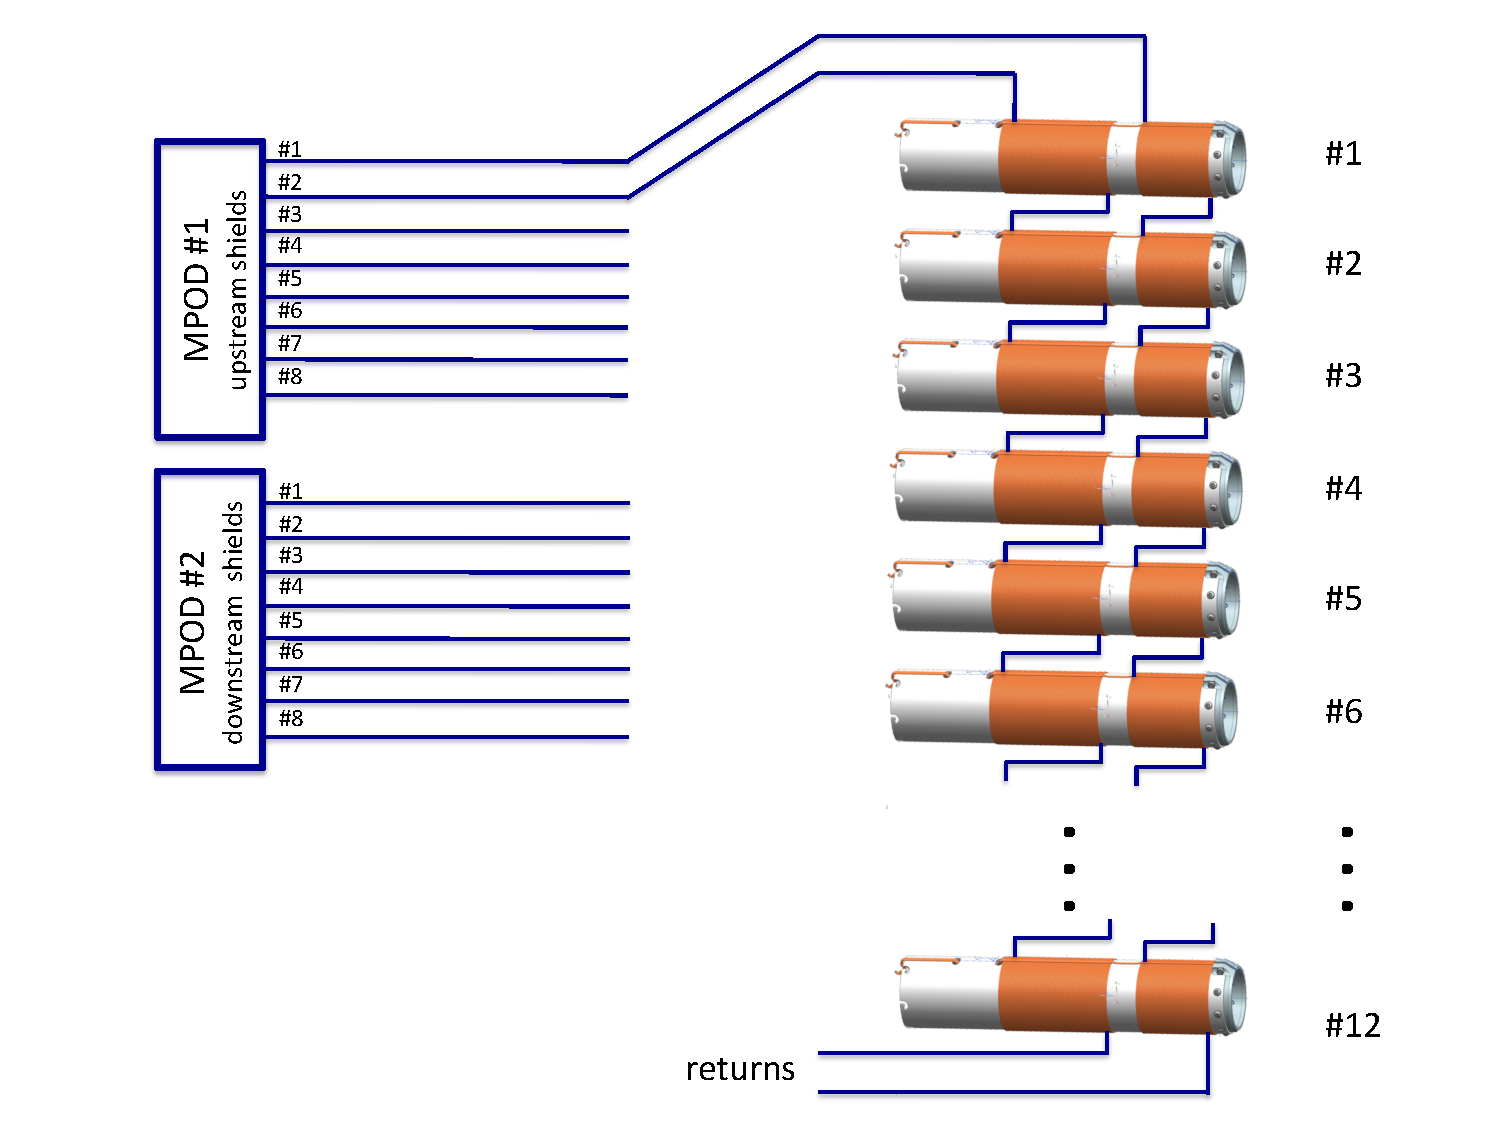
\includegraphics[angle=-90,width=0.70\textwidth,natwidth=610,natheight=642,angle=90]
{pics/compensation-coils.pdf}}}
\end{picture} 
\caption{(Color Online) Layout of the power circuit for the CTOF magnetic shield compensation coils.}
\label{coils}
\end{figure}
%%%%%%%%%%%%%%%%%%%%%%%%%%%%%%%%%%%%%%%%%%%%%%%%%%%%%%%%%

Although the Wiener MPOD system can provide up to 5~A per channel, our field test studies
(see Section~\ref{shield-testing}) showed that typical coil currents of the level of 0.5~A
to 1~A were appropriate for shield operation. In this current regime the coil system remains
at room temperature. During operation of the coil power supply in Hall~B, a temperature
interlock circuit protects the coils from overheating by shutting off the MPOD power supply if
the shield temperature at the mandrel location goes about 100~$^{\circ}$F.

\subsubsection{Model Calculations}

In order to optimize the performance of the CTOF magnetic shields, studies were performed 
using both 2-D and 3-D finite element analysis (FEA) calculations. Ultimately, full 
consistency between these approaches was achieved~\cite{cn2015-003}. The 2-D FEA calculations 
were carried out using the Poisson Superfish program~\cite{poisson}. In this model the shield 
was placed into an axial field with a gradient along the shield axis to approximate a realistic 
CLAS12 field scenario. For this calculation the maximal external field was $\sim$1300~G at the 
side of the shield nearest the solenoid and $\sim$700~G at the opposite end. The magnetic field 
in the accelerating area of the PMT was below 1~G without the compensation coils energized. 

Full 3-D calculations with the OPERA-TOSCA suite~\cite{opera} for the CTOF shields in a 1~kG
uniform external field titled at 40$^\circ$ with respect to the shield axis yielded the results 
shown in Figs.~\ref{shield-opera1} and \ref{shield-opera2}. Fig.~\ref{shield-opera1} plots the 
field profile as a function of transverse coordinate across the shield system at the location 
of the photocathode, the first dynode, and the middle of the accelerating structure. 
Fig.~\ref{shield-opera2} plots the field profile as a function of axial coordinate along the 
shield system. The different curves correspond to coordinates near the inner cylinder 
walls and along the PMT symmetry axis.

Fig.~\ref{shield-opera1} shows that as the outer shield layer is approached moving toward the
PMT, the field magnitude slightly changes and that the behavior depends on the coordinate along 
the axis. Inside the outer ferromagnetic layer, the field magnitude rises up by a factor of 
10 to $>10^4$~G due to the very high magnetization of the ferromagnetic material that may be 
close to saturation. In the region between the outer and middle ferromagnetic cylinders, the 
field magnitude drops by a factor of 10-50 depending on the axial coordinate along the shield. 
A similar effect is seen between the middle and the inner layers. At the location of the PMT 
the field magnitude is $\sim$0.4~G. Note that the compensation coils were not energized for 
these calculations. 

%%%%%%%%%%%%%%%%%%%%%%%%%%%%%%%%%%%%%%%%%%%%%%%%%%%%%%%%%
\begin{figure}[htbp]
\vspace{6.0cm}
\begin{picture}(50,50) 
\put(0,-40)
{\hbox{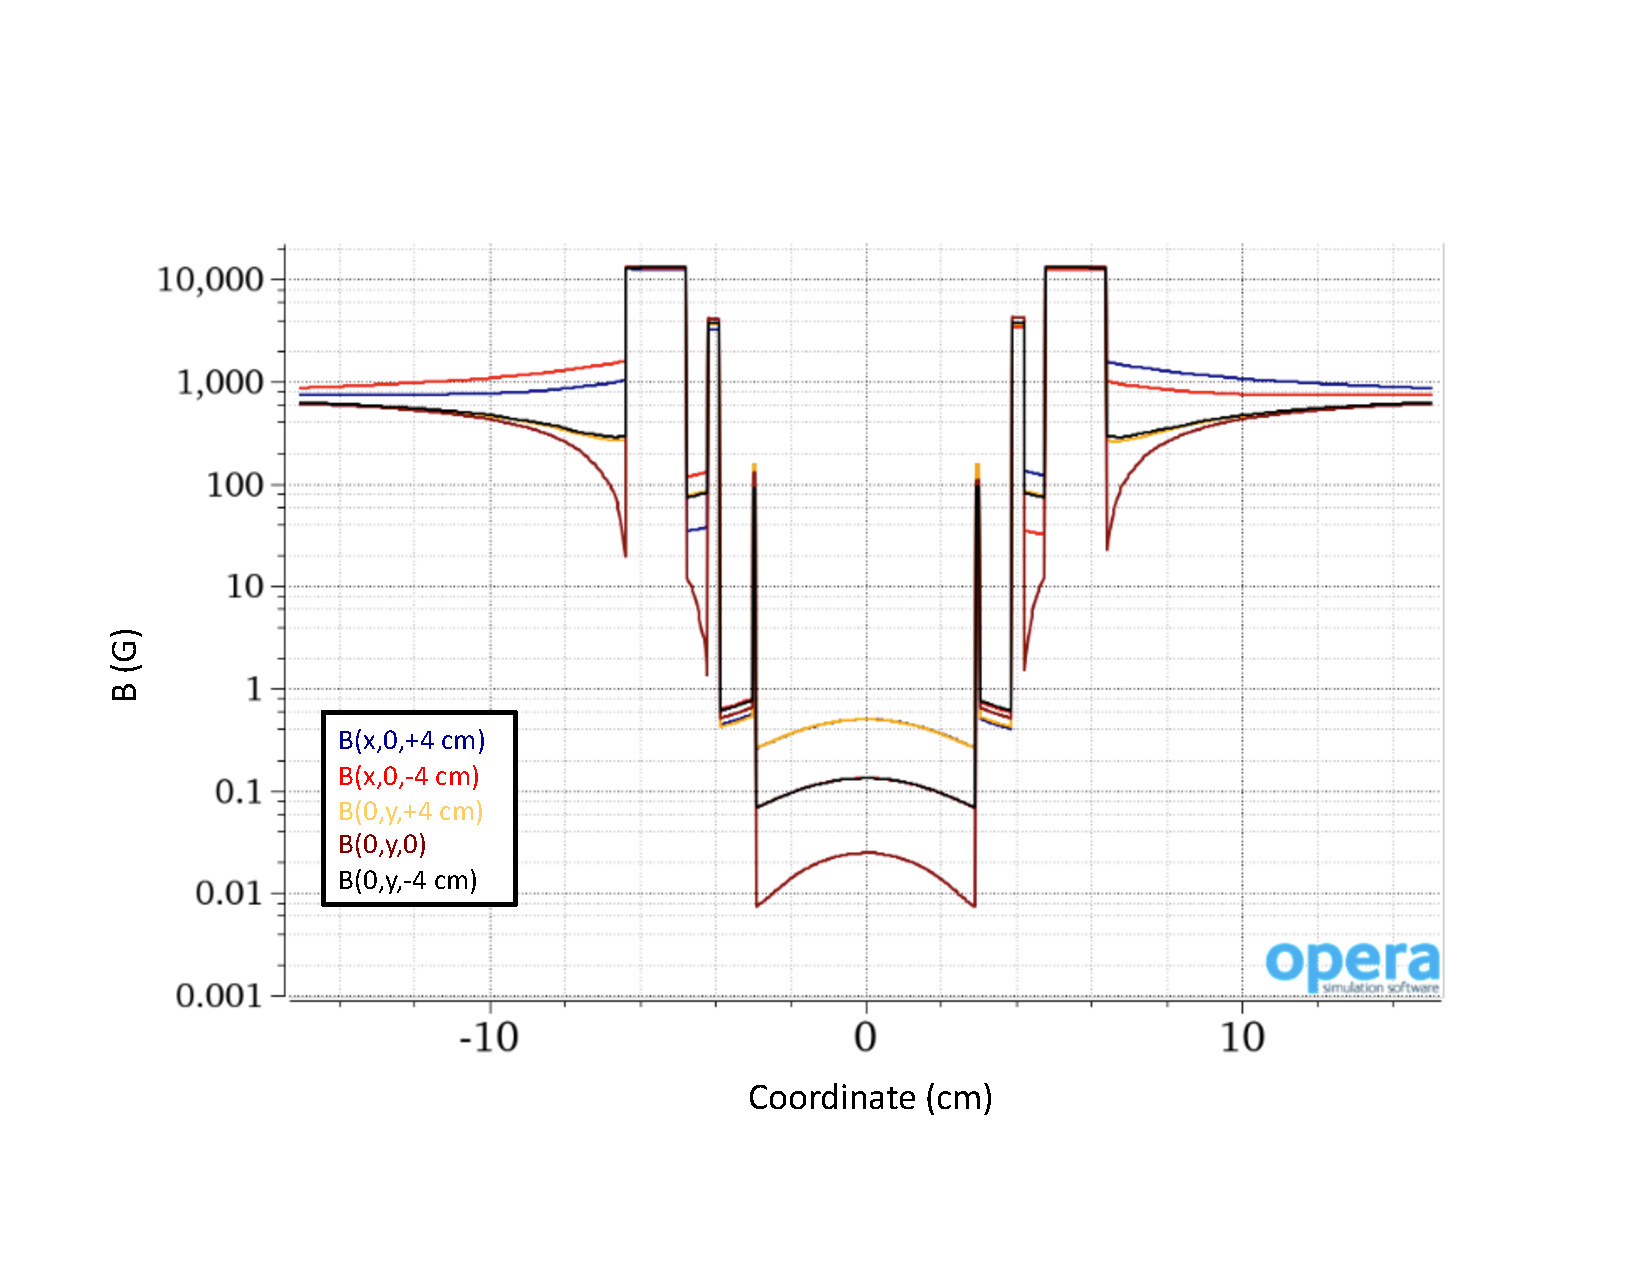
\includegraphics[width=0.80\textwidth,natwidth=610,natheight=642]{pics/opera-mod1a.pdf}}}
\end{picture} 
\caption{(Color Online) 3-D magnetic field calculations using the code suite Opera~\cite{opera} for
the CTOF PMT shield in a uniform 1~kG field. The calculation plots the field profile (in G) across the 
transverse coordinate (in cm) of the CTOF three-layer passive magnetic shield system. The different
curves correspond to different transverse coordinates along the PMT (photocathode at $z$=+4~cm,
first dynode at $z$=0, and middle of the accelerating structure at $z$=-4~cm). For this calculation the
external field lines were at an angle of 40$^\circ$ relative to the shield axis of symmetry to reflect the
expected operational configuration of the shields.} 
\label{shield-opera1}
\end{figure}
%%%%%%%%%%%%%%%%%%%%%%%%%%%%%%%%%%%%%%%%%%%%%%%%%%%%%%%%%

Fig.~\ref{shield-opera2} shows an essentially monotonic decrease of the field strength moving
along the axial coordinate that contains the shield toward the region where the PMT is located. 
The calculations show that the remnant field at any position within the PMT accelerating area 
($\pm$4~cm about 0) is below 0.5~G. Again this calculation was performed with the compensation 
coils turned off.

%%%%%%%%%%%%%%%%%%%%%%%%%%%%%%%%%%%%%%%%%%%%%%%%%%%%%%%%%
\begin{figure}[htbp]
\vspace{5.5cm}
\begin{picture}(50,50) 
\put(0,-40)
{\hbox{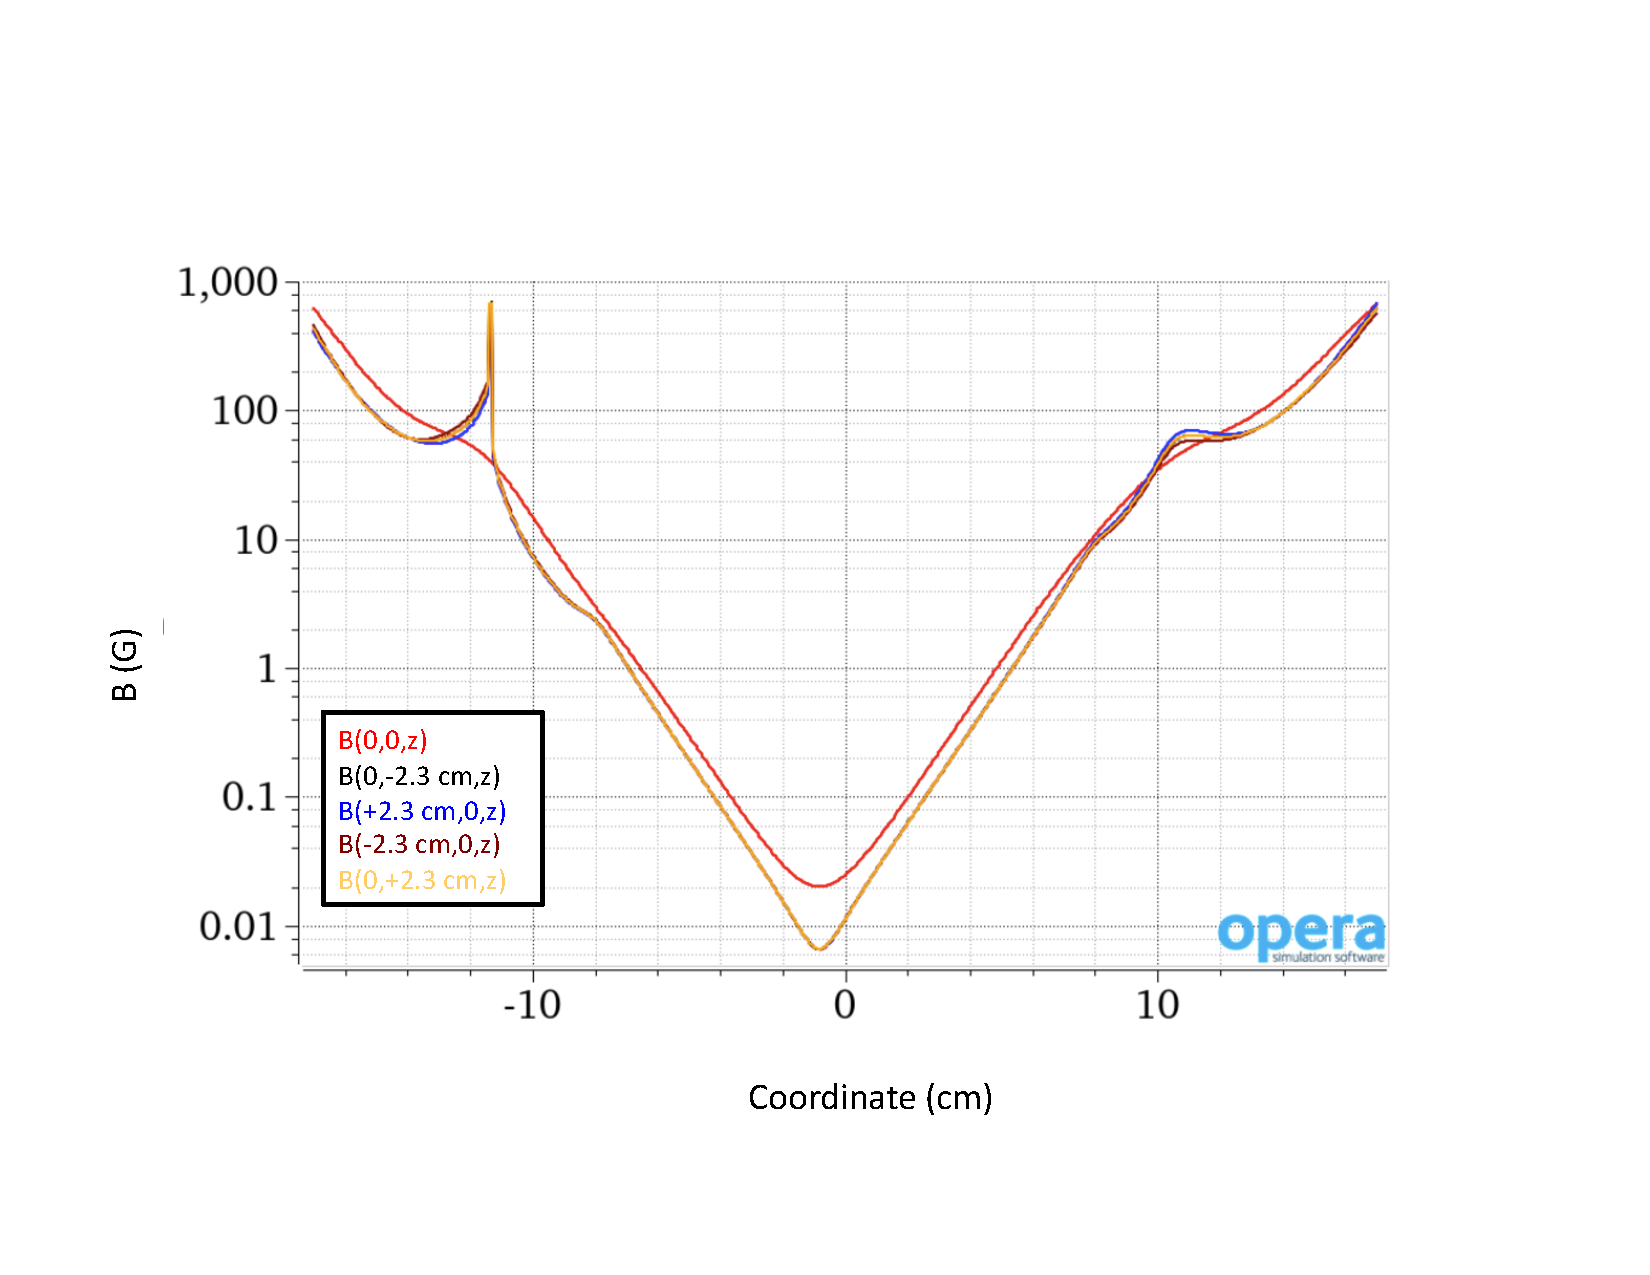
\includegraphics[width=0.80\textwidth,natwidth=610,natheight=642]{pics/opera-mod2a.pdf}}}
\end{picture} 
\caption{(Color Online) 3-D magnetic field calculations using the code suite Opera~\cite{opera} for
the CTOF PMT shield in a uniform 1~kG field. The calculation plots the field profile (in G) at coordinates 
across different axial lines at $y=\pm$2.3~cm. For this calculation the external field lines were at an
angle of 40$^\circ$ relative to the shield axis of symmetry to reflect the expected operational
configuration of the shields.}
\label{shield-opera2}
\end{figure}
%%%%%%%%%%%%%%%%%%%%%%%%%%%%%%%%%%%%%%%%%%%%%%%%%%%%%%%%%

\subsubsection{Shield Testing}
\label{shield-testing}

In order to validate the 2-D and 3-D FEA calculation results for the CTOF magnetic shield
design, studies were completed placing one of the shields in the fringe field of a 5-T 
superconducting test magnet (30~cm long, 12.7~in diameter bore). For these tests the goal was 
to place the CTOF shield in the fringe field at positions that matched the field strength and 
gradient for what was expected from Table~\ref{field-position} for the shield positioning in 
the fringe field of the CLAS12 solenoid. Tests were performed in field conditions that well 
matched those expected for the high-pitch angle and low-pitch angle upstream PMTs. The full
results from these tests are detailed in Ref.~\cite{shield-test}. Note that the downstream CTOF
PMTs are positioned in a region of the solenoid fringe field that is more than a factor of two lower 
than for the upstream PMTs. For this reason this configuration was not studied.

The first set of measurements was carried out with the compensation coils turned off to evaluate
the passive shield layers. The data collected clearly show the efficacy of the shield system design.
The tests showed that all field components were measured to be less than 0.5~G at all positions
along the PMT volume. Studies of the effect of the compensation coils on affecting the internal field
along the PMT location were completed with coil current settings of up to 1~A (with $i_{z_1} = i_{z_2}$).
The studies showed that the compensation coils could be adjusted to reduce the internal remnant
fields to levels of $\sim$0.2~G even in the studies with up to nearly two times higher external fields.

\subsection{Assembly}
\label{assembly}
           
The CTOF counter assembly employed a precision alignment table configurable to match the geometry
of the CTOF counters with both the high-pitch angle and the low-pitch angle upstream light guides. This
assembly table was designed to position the counter light guides and scintillation bar into their proper
alignment for gluing. To bond the pieces together Bicron BC-600 optical cement~\cite{bc600-ref} was
employed. Each counter was left to cure for 24~hours after application of the epoxy. Note that our
bench tests showed that the scintillator/light guide joints made up with BC-600 were 30\% stronger
than using Dymax 3-20262 UV curing glue~\cite{dymax}.

After gluing of the counters was completed, they were placed onto storage carts in the CTOF assembly
area. These carts each held eight counters laid horizontally in a vertical stack with $\sim$20~cm
between each counter. The next step in the counter preparation was to wrap the counters, first in a highly
reflective layer and then in a fully opaque layer. The highly reflective wrapping layer for the CTOF counters
employs the Enhanced Specular Reflector VM-2002~\cite{vm2002-ref}. This layer serves to increase the
light transmittance along the counter from the charged particle ionization path to the PMTs. The outer
opaque layer for the CTOF counters employs Tedlar, a polyvinyl fluoride film from DuPont~\cite{dupont-ref}.

The nominal gap between the bare faces of neighboring CTOF scintillation bars in the barrel is
800~$\mu$m. In order to have sufficient space to form the barrel at its nominal radial position allowing
for assembly and component tolerances, it was imperative that the wrapping be completed so that there
were no wrinkles or excess material on the inter-counter sides of the bars and that all tape seals were
applied only to the inner and outer radial surfaces of the bars. To aid in this required the VM-2002 sheets
to be pre-formed using templates that made precise creases that matched the wedge-shape of the
scintillation bars of the two different designs (low-pitch angle bar and high-pitch angle bar - see
Section~\ref{geometry}).

The scheme for wrapping the Tedlar layer on the scintillation bars was based on cold-forming 
Tedlar templates using tooling designed to give precise Tedlar forms that could be mated to the 
counters and sealed with electrical tape along smooth, wrinkle-free seams.  This region covers the 
scintillation bar and $\sim$30.5~cm of the transitions from the tapered to the cylindrical portions
of the upstream and downstream light guides. The remaining portions of the Tedlar wrapping that 
span from the template region of the counters to the PMTs was easily covered using rectangular 
pieces of Tedlar wrapped around the cylindrical light guides. The full details on the counter 
wrapping for the scintillation bars is included in Ref.~\cite{ctof-wrapping}. The final inter-counter
gap after wrapping is $\sim$450~$\mu$m on average (= 800~$\mu$m - 2$\times$50.8~$\mu$m
(Tedlar outer-wrap) - 4$\times$66.0~$\mu$m (VM-2002 inner-wrap including overlap of sheets)).

After the counter wrapping was completed, the counters were secured in their positions on the
storage carts and the magnetic shields were installed. Due to the weight of the shield assemblies,
they were designed to be assembled for counter testing without the heavy steel cylinder and its
associated upstream steel cone (see Fig.~\ref{bshield-3d}). These pieces were not attached to the
counters until they were moved to Hall~B for installation into the solenoid using the CTOF installation
strongback that supported the weight of the shields. The installation procedure for the counters is
detailed in Section~\ref{installation}. Full details on the procedures for assembly of the CTOF
magnetic shields are included in Ref.~\cite{ctof-sh-assy}.

With the inner and intermediate shield layers installed on each light guide, the final step of the
counter assembly was to install the R2083 PMTs with their voltage dividers into the shield volume.
Note that the azimuthal orientation of the PMT within the Co-NETIC shield layer takes is set to
minimize $\vec{v} \times \vec{B}$ effects from the remnant solenoid field within the shield volume
that might otherwise result in loss of photoelectrons from the acceleration chain. The coupling contact
between the PMT and the end of the light guide was made up with BC-630 silicone optical grease
\cite{bc-630} ($n$=1.465) to match the indices of refraction of the two materials. The PMT was held
against the light guide using pressure from a spring clamp at the end of the voltage divider (see
Fig.~\ref{bshield-3d}).

The storage carts served as the basis for the CTOF cosmic ray test stand and extensive 
characterization of the counters and their performance were completed during the year between 
the completion of counter assembly and installation in Hall~B. The results of the cosmic ray 
studies in the assembly area are detailed in Section~\ref{sec:performance}.

\subsection{Installation}
\label{installation}

Due to the geometry of the CTOF counters, they were inserted into the solenoid magnet one at a 
time, with the insertion taking place from the downstream end of the solenoid. The counter 
installation consisted of four steps as detailed below and illustrated in Fig.~\ref{install}.

Step \#1: The counter was placed on the heavy shield attachment table and the outer steel shield
cylinders were installed. The installation strongback was attached to the counter. The full shield 
assemblies were fully supported by the strongback with no stress on the counter itself. The 
counter was then craned from the floor of Hall~B and the strongback was attached to the installation
arm of the CTOF installation cart that moved along a set of rails used for moving the solenoid magnet.
Initially the cart was moved well downstream of the solenoid (which had been moved $\sim$10~m
upstream of its nominal operating position). The counter and strongback were supported on the
installation arm pivoted to the counter installation position as shown in Fig.~\ref{install}(a).

Step \#2: The cart was moved upstream to insert the counter into the solenoid volume. The
installation arm was then rotated to the desired azimuthal location after the cart hit the rail stop
positioned along the solenoid rails at the proper installation position as shown in Fig.~\ref{install}(b).

Step \#3: The counter installation arm was then pivoted until the CTOF scintillation bar was horizontal
and the pieces that mate with the support structure matched up and engaged as shown in Fig.~\ref{install}(c).

Step \#4: The load of the shields was transferred from the strongback to the CTOF support structure.
The attachment bolts were engaged through slots in the support structure that allowed for the counter to
be adjusted to its final position. The strongback was then freed and the installation arm was pivoted back
to its insertion position, allowing the cart to be pushed back downstream and reset for the next counter as
shown in Fig.~\ref{install}(d).

%%%%%%%%%%%%%%%%%%%%%%%%%%%%%%%%%%%%%%%%%%%%%%%%%%%%%%%%%
\begin{figure}[htbp]
\vspace{6.2cm}
\begin{picture}(50,50) 
\put(15,260)
{\hbox{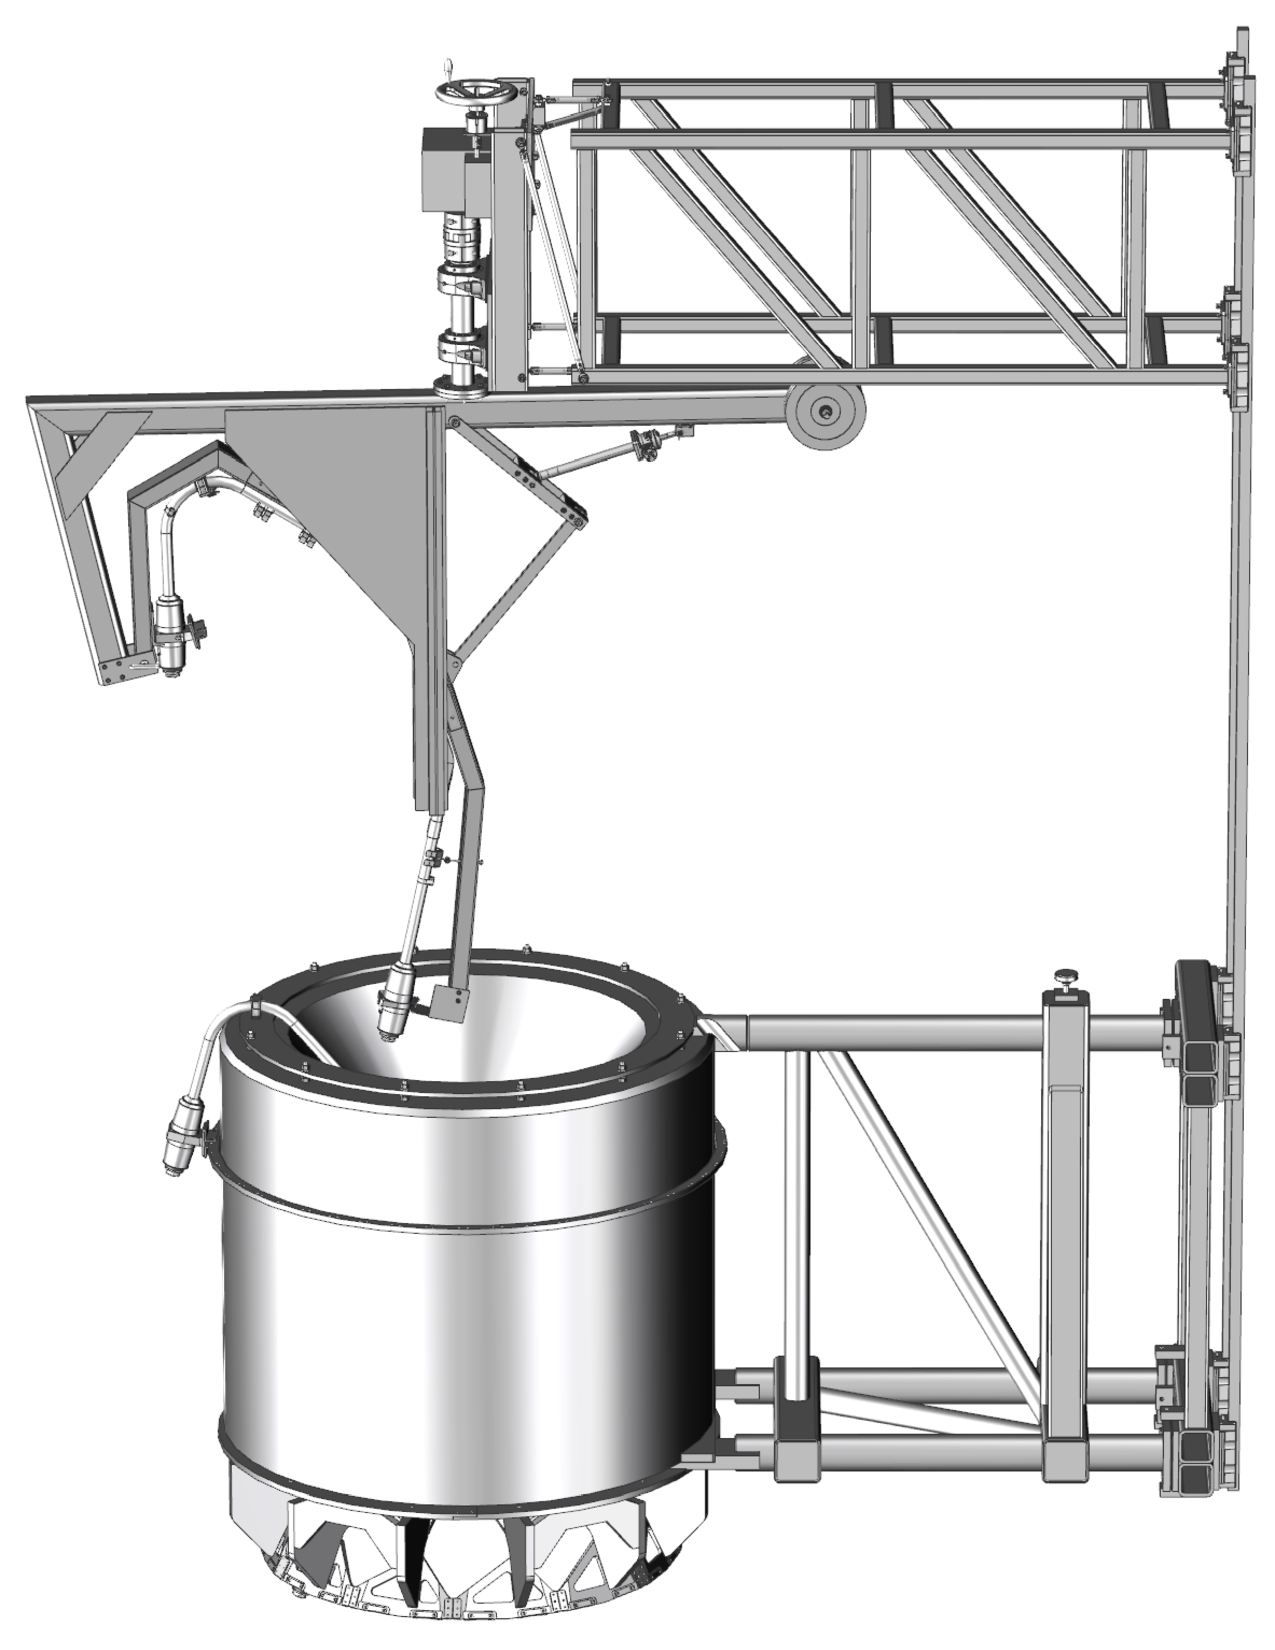
\includegraphics[angle=-90,width=0.35\textwidth,natwidth=610,natheight=642]{pics/ctof_nim_19e.pdf}}}
\put(210,260)
{\hbox{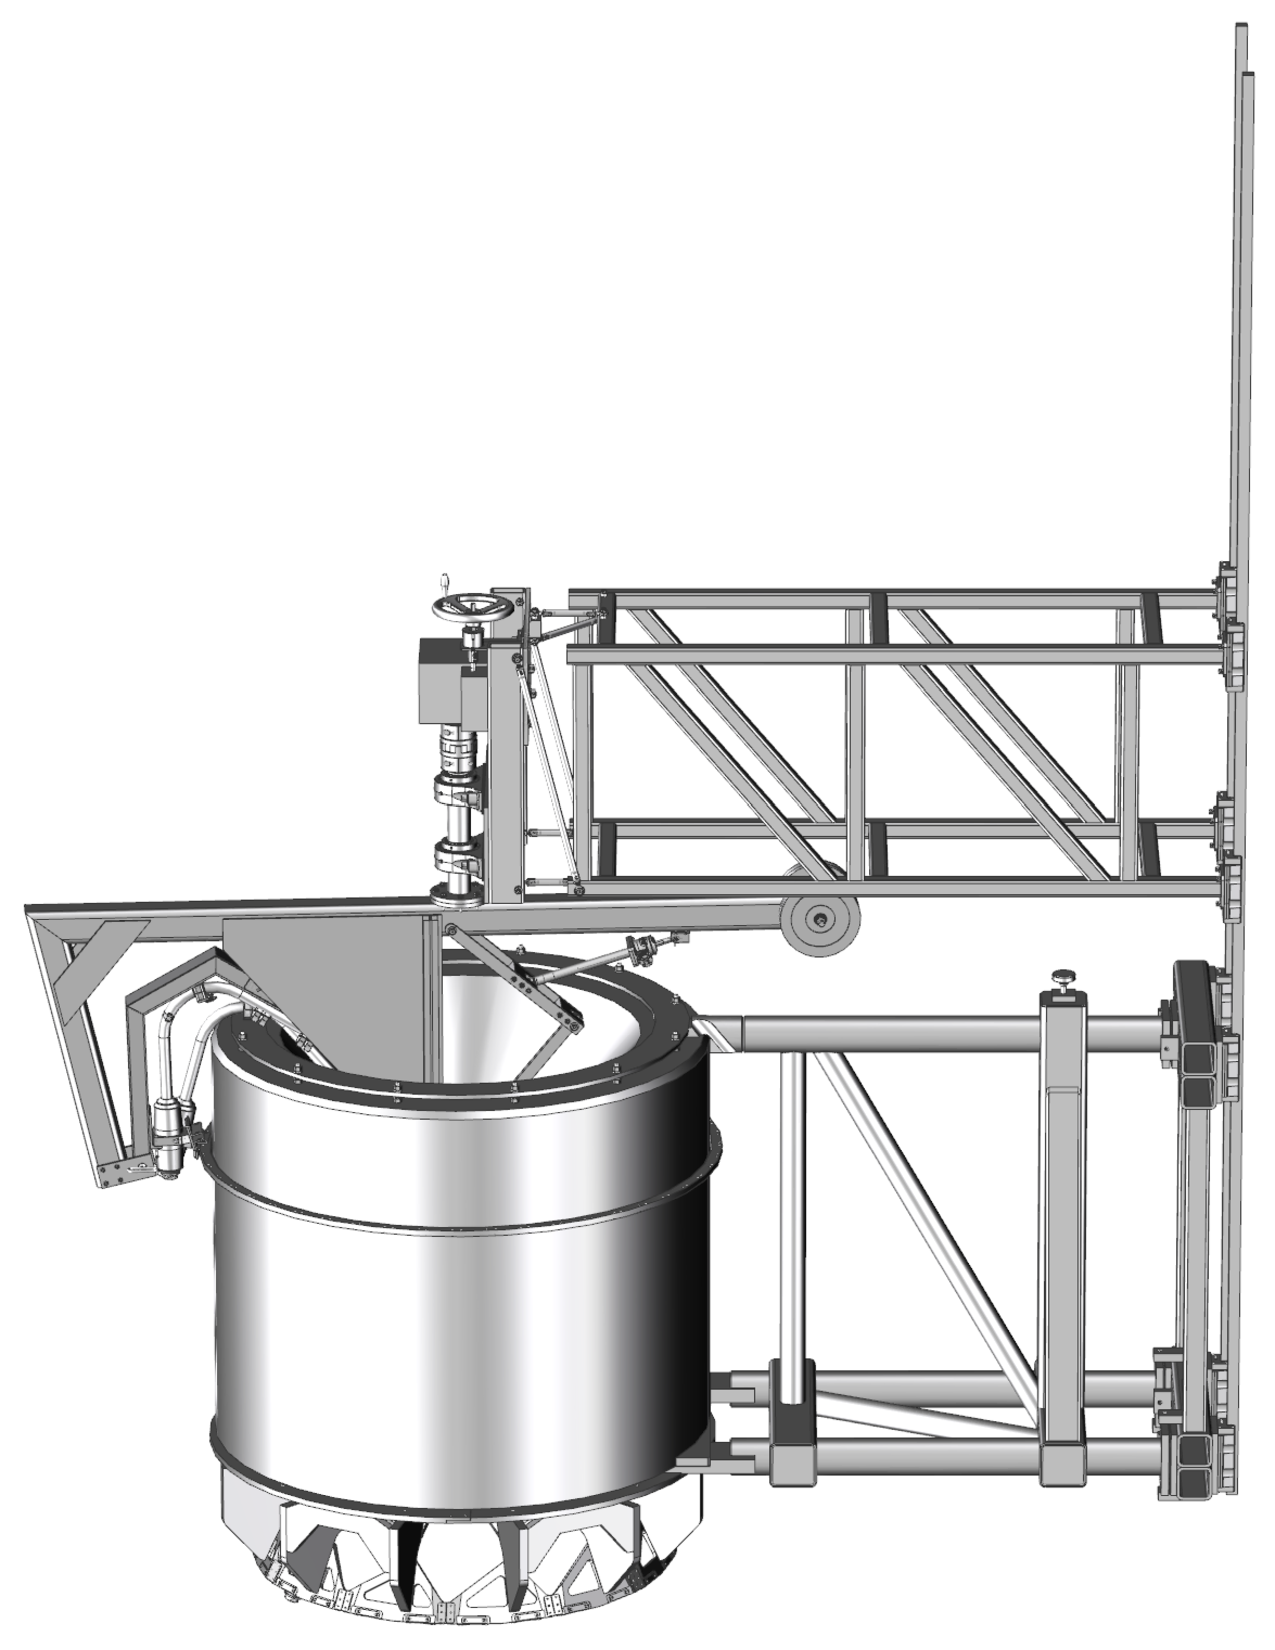
\includegraphics[angle=-90,width=0.35\textwidth,natwidth=610,natheight=642]{pics/ctof_nim_19g.pdf}}}
\put(15,125)
{\hbox{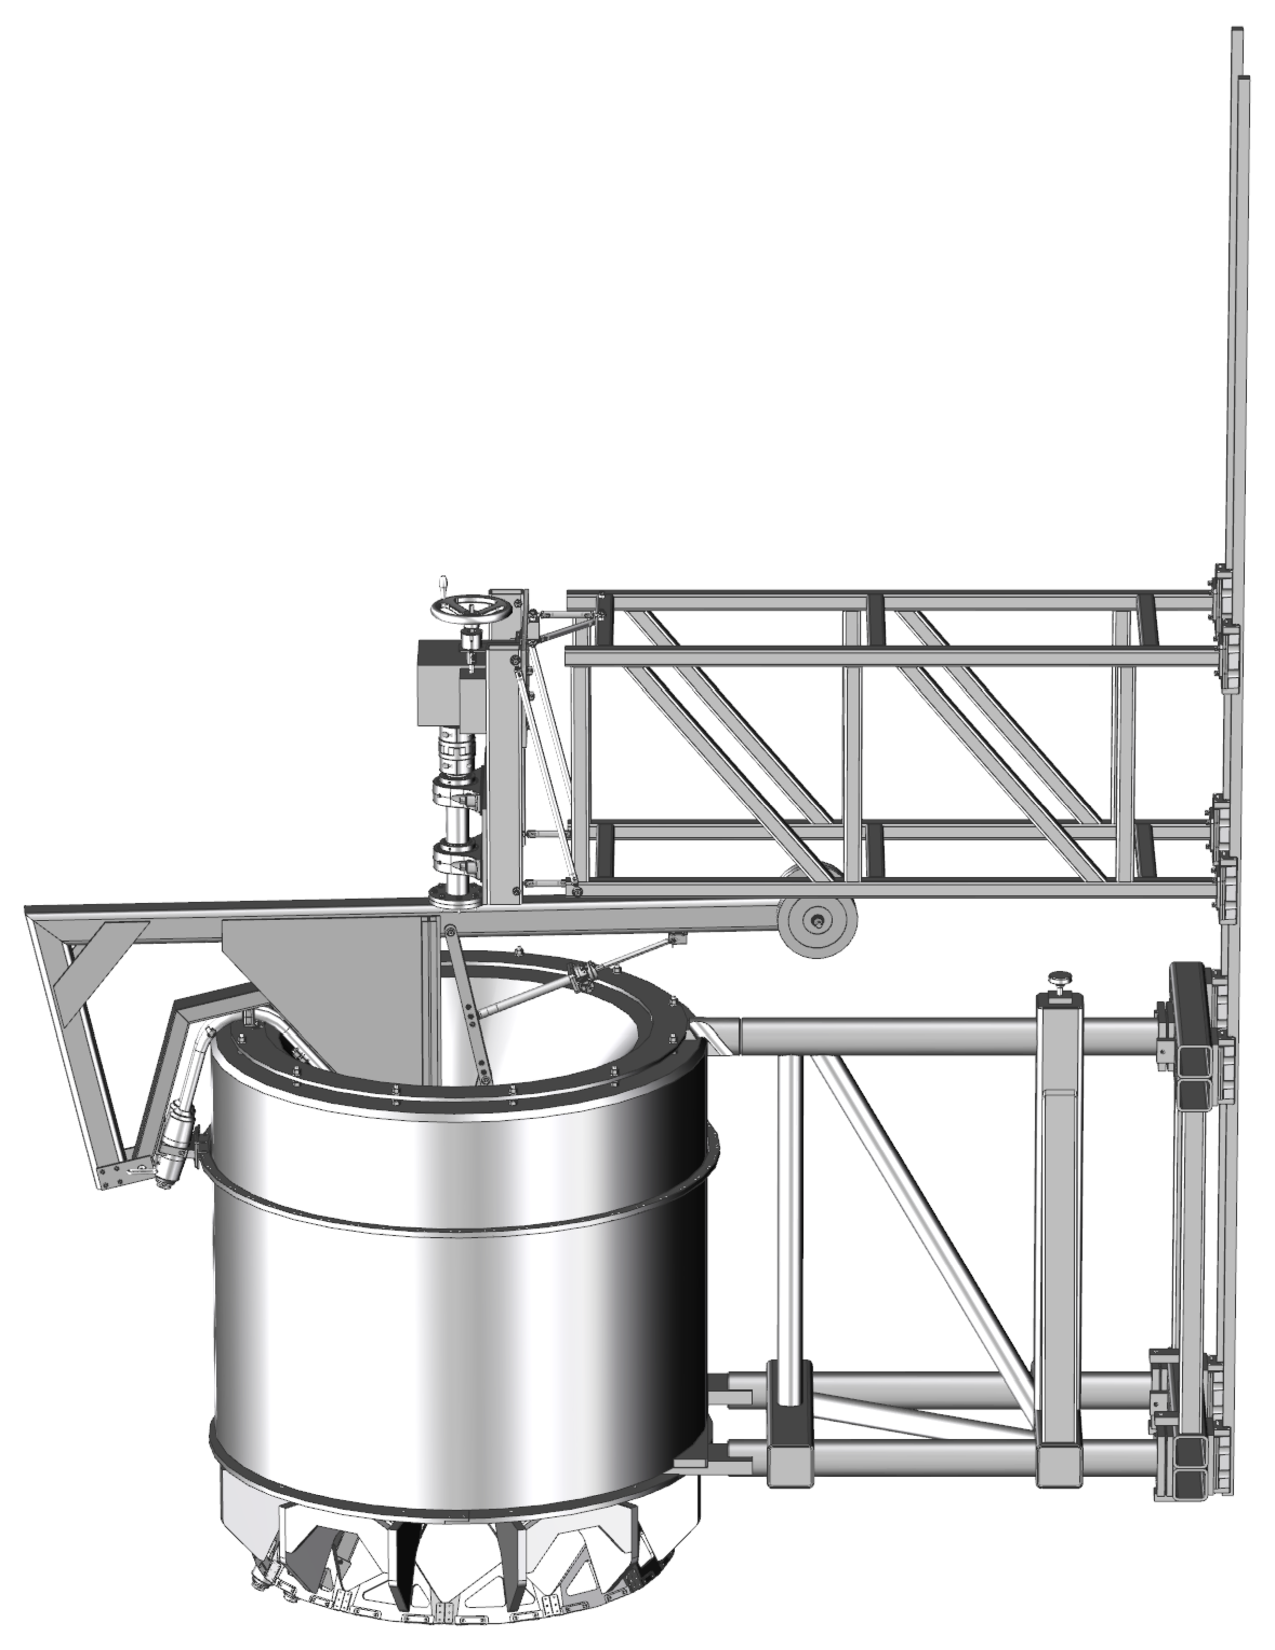
\includegraphics[angle=-90,width=0.35\textwidth,natwidth=610,natheight=642]{pics/ctof_nim_19h.pdf}}}
\put(210,125)
{\hbox{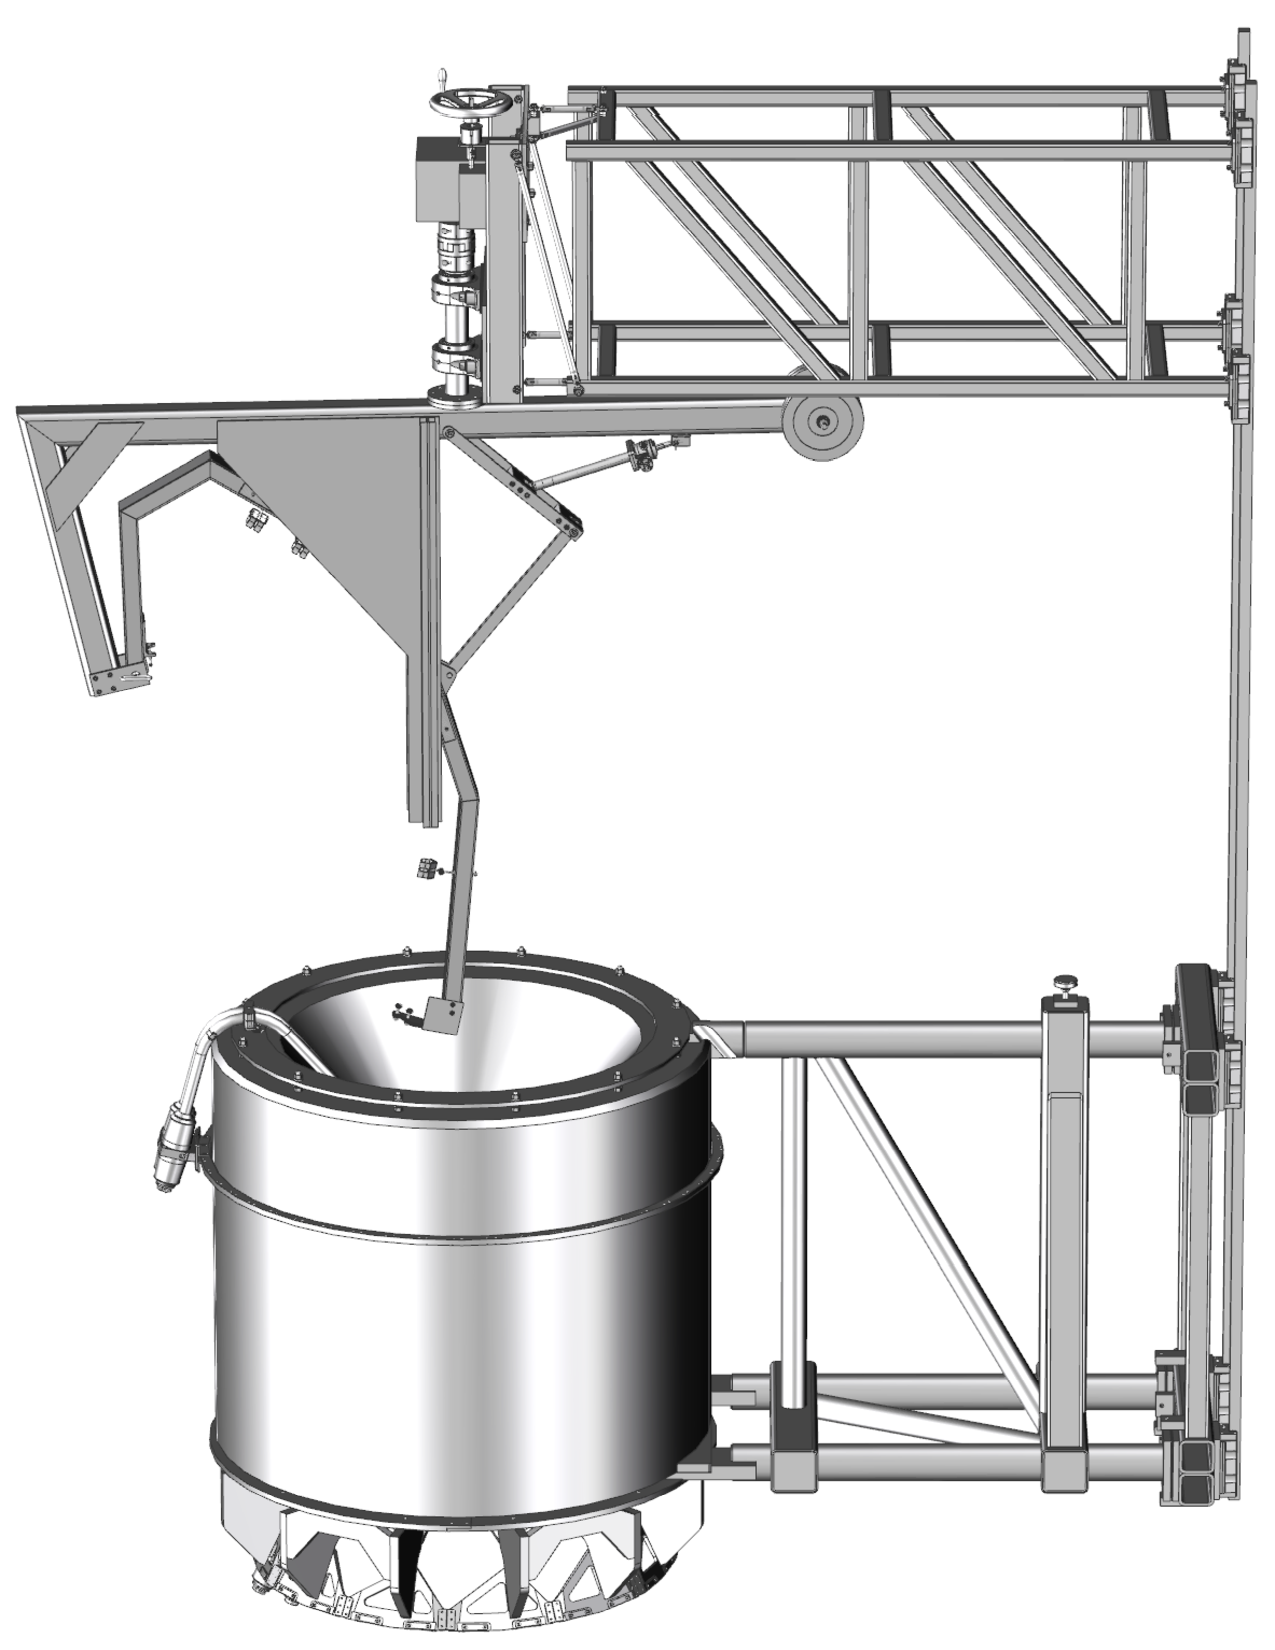
\includegraphics[angle=-90,width=0.35\textwidth,natwidth=610,natheight=642]{pics/ctof_nim_19j.pdf}}}
\end{picture} 
\caption{Steps in the CTOF counter installation sequence. (a) Mount counter to installation cart, (b) Move
counter into solenoid from the downstream end and rotate in azimuth to proper position, (c) Pivot counter
radially into proper installation position, (d) Attach the counter to the support structure and pull cart out of
solenoid.}
\label{install}
\end{figure}
%%%%%%%%%%%%%%%%%%%%%%%%%%%%%%%%%%%%%%%%%%%%%%%%%%%%%%%%%

The installation sequence proceeded with installing the counters in quadrants, starting at the bottom
position on the solenoid and installing counters alternating back and forth between the high-pitch
angle and low-pitch angle designs. The final counter for insertion (with the low-pitch angle design) was
machined to have a rectangular cross section of 24~cm width to fit into the last gap in the barrel.

After installation of each counter, survey measurements were taken to ensure counter positioning 
was within tolerances and any adjustments necessary were made. The final survey of the counters
after installation and adjustments showed that all counters were positioned radially to within $\pm$3~mm
of their design position. The final counter-by-counter radial offsets were included in the CTOF geometry
tables used for event reconstruction. The signal and high voltage cables were attached after all counters
were installed. This was followed by attachment of the power connections to the magnetic shield compensation
coils.

\subsection{Electronics}
\label{sec-elec}

The CTOF counters generate prompt signals for pulse-height and timing analysis. The anode from 
each PMT is connected to a passive signal splitter. 20\% of the anode pulse is fed to a JLab-designed
analog-to-digital converter flash ADC (FADC). 80\% of the anode pulse is fed to a constant fraction
discriminator connected to a high-resolution time-to-distance converter (TDC). The overall layout of
the CTOF electronics that processes these signals is shown in Fig.~\ref{electronics}.

%%%%%%%%%%%%%%%%%%%%%%%%%%%%%%%%%%%%%%%%%%%%%%%%%%%%%%%%%
\begin{figure}[htbp]
\vspace{5.8cm}
\begin{picture}(50,50) 
\put(40,-20)
{\hbox{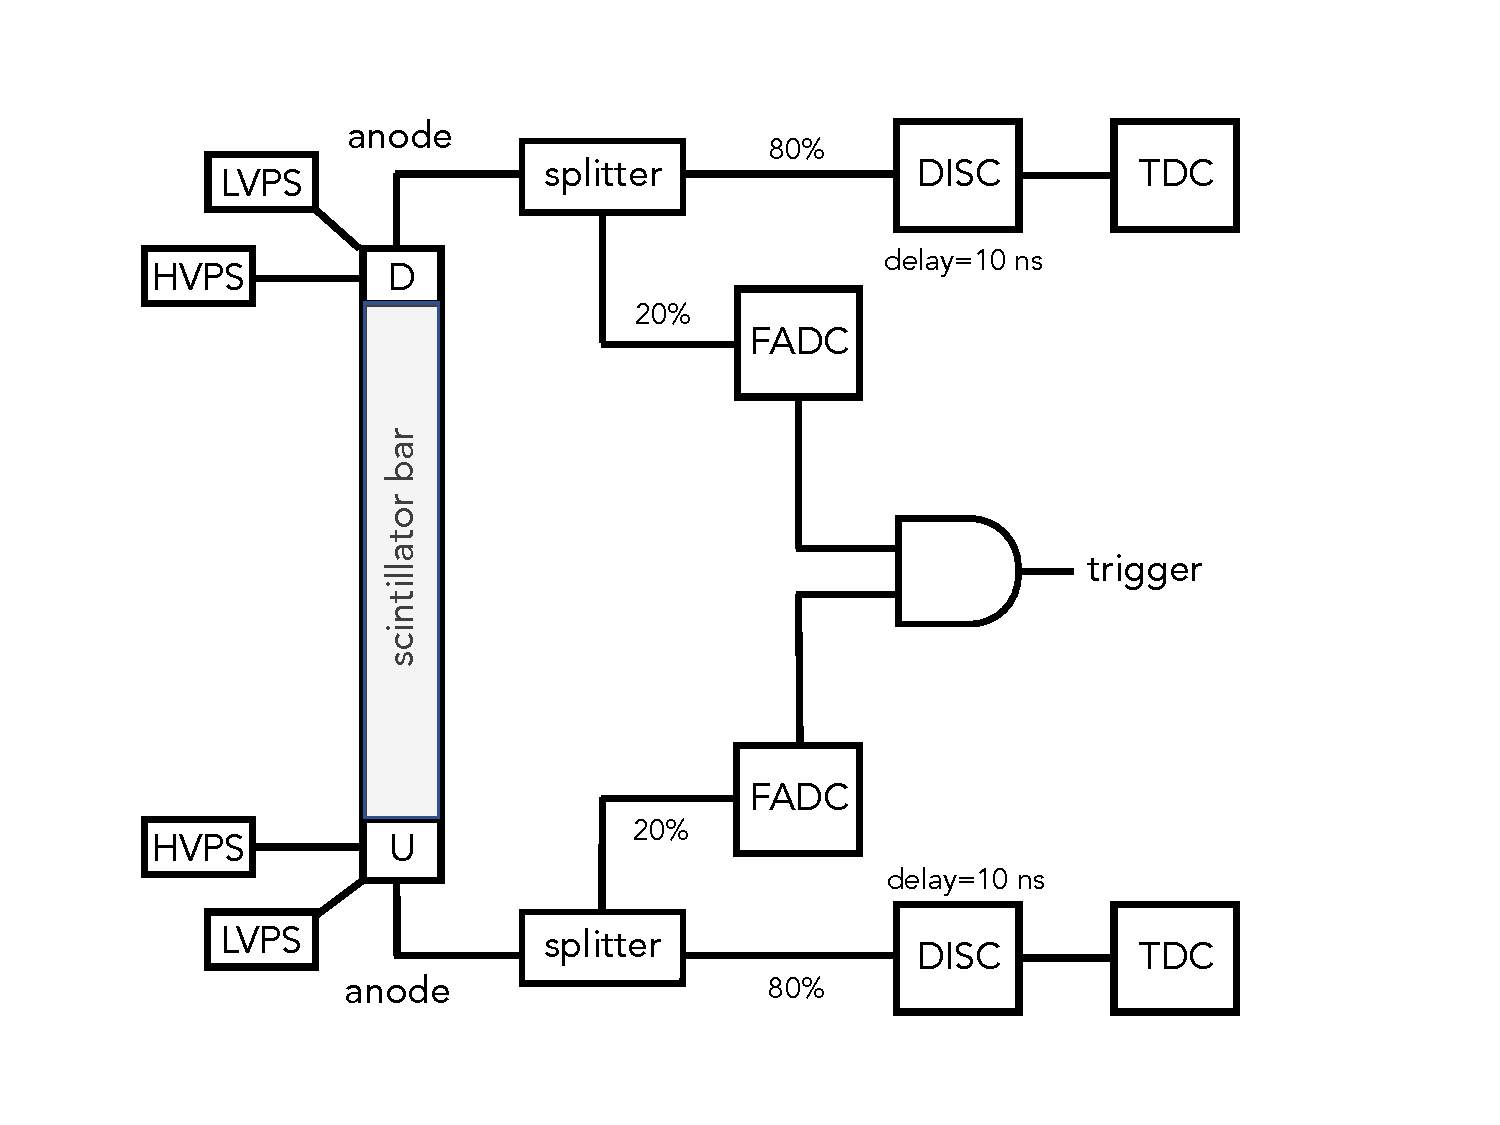
\includegraphics[width=0.7\textwidth,natwidth=610,natheight=642]{pics/ctof-electronics-block.pdf}}}
\end{picture} 
\caption{Block diagram showing the layout of the readout electronics and power connections for a single
CTOF counter.}
\label{electronics}
\end{figure}
%%%%%%%%%%%%%%%%%%%%%%%%%%%%%%%%%%%%%%%%%%%%%%%%%%%%%%%%%

Due to the limited number of channels in the CTOF system, the decision was made to employ constant
fraction discriminators (CFDs) for the readout. The constant fraction technique permits optimal timing
measurements to be made without the need for sizable offline time-walk corrections to remove the
effects of time offsets due to pulses of different amplitudes crossing threshold at different times.

For the CTOF system Ortec 935 4-channel 100~MHz CFDs~\cite{ortec-ref} are employed. The
single-width NIM modules accept negative input pulses and generate three simultaneous NIM-standard
fast negative logic pulses for each input pulse that exceeds the set threshold level. The unused bridged
outputs are terminated into 50~$\Omega$ as recommended by the manufacturer.

The constant-fraction shaping delay for each discriminator channel is determined by the length of
external 50~$\Omega$ coaxial cable connected to the channel shaping circuit. To select the optimal
shaping delay the counter timing resolutions were studied for delay cables from 4~ns to 16~ns for
each counter relative to a fixed reference time. Fig.~\ref{cfd-study}  shows the results of these
studies for a set of 8 counters. The resolution was seen to improve until a minimum is reached and
then remains relatively flat. The final delay setting employed 10~ns delay cables (with the internal
module offset delay omitted) with the time-walk compensation network setup according to the
manufacturer's recommendations.

%%%%%%%%%%%%%%%%%%%%%%%%%%%%%%%%%%%%%%%%%%%%%%%%%%%%%%%%%
\begin{figure}[htbp]
\vspace{4.3cm}
\begin{picture}(50,50) 
\put(70,-180)
{\hbox{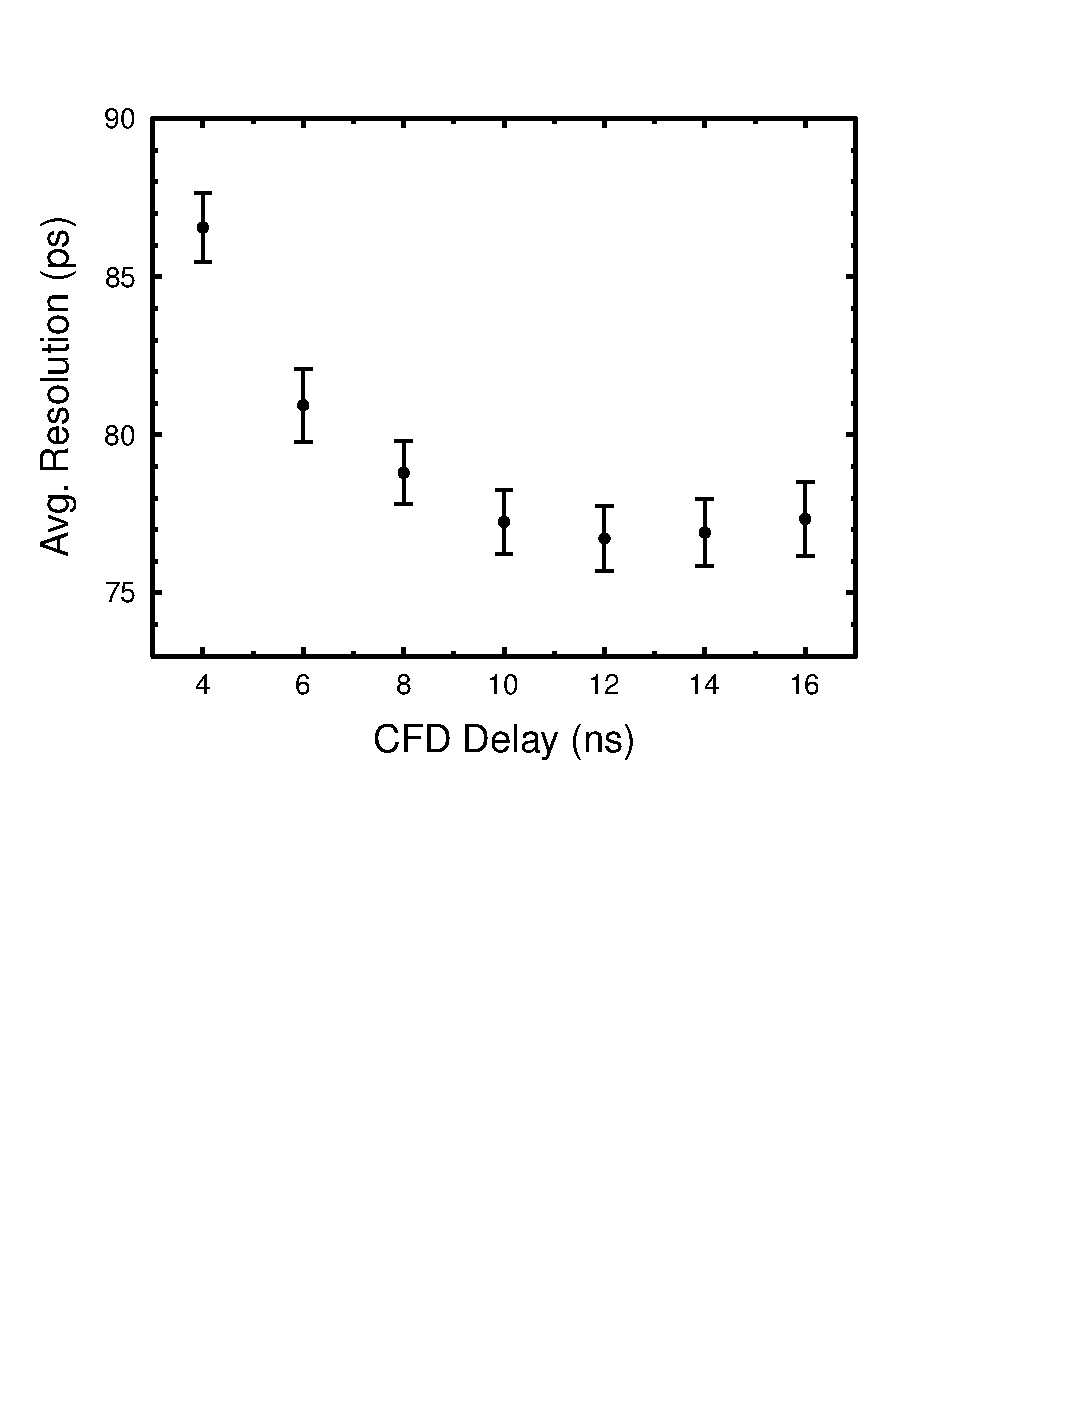
\includegraphics[width=0.85\textwidth,natwidth=610,natheight=642]{pics/res-comp19b.pdf}}}
\end{picture} 
\caption{Average resolution for a set of 8 CTOF counters (ps) vs. CFD shaping delay (ns).}
\label{cfd-study}
\end{figure}
%%%%%%%%%%%%%%%%%%%%%%%%%%%%%%%%%%%%%%%%%%%%%%%%%%%%%%%%%

During operation of the CTOF system in Hall~B, the CTOF discriminator thresholds were set to
$\sim$30~mV. After setting the PMT gains, this corresponded to a threshold of $\sim$1~MeV of
deposited energy. This threshold is well below the 6~MeV energy deposited by a normally incident
minimum-ionizing particle.

The output of the discriminator goes to a CAEN VX1290N 16-channel 25~ps LSB (least significant bit)
VME TDC~\cite{tdc-manual}. These multi-hit pipeline TDCs were chosen in order to allow for readout
capability in the operating luminosity of $1 \times 10^{35}$~cm$^{-2}$s$^{-1}$. The TDC readout window
was set to 250~ns to ensure the full dynamic range of the data was safely in time with the trigger. The
key performance specifications of these units are given in Table~\ref{tdcadc-specs}.

The integral non-linearity (INL) of the TDCs represents the accumulated error of the input-output
characteristic of the TDC with respect to the ideal response. This is defined by the function:

\begin{equation}
D(t) = \int \frac{t}{LSB},
\end{equation}

\noindent
where $D$ is the output data, $t$ is the input time, and $LSB$ is the bin size. The compensation tables
for the CAEN V1190A and VX1290A TDCs are stored as tables in the unit SRAM memory. Initial tables
are measured at the factory and come preloaded on the modules. These tables are reasonably accurate
when reading out the module using its internal 40~MHz/25~ns period clock. However, in CLAS12, the
modules are strobed with a clock of a slightly larger frequency of 41.67~MHz. This difference in the
frequency has a non-negligible affect the INL tables. For our purposes we use a high frequency pulser to
populate the full dynamic range of the TDC within the CLAS12 readout clock. The measured INL tables that
were derived from this calibration were written into the TDC memory to replace the factory-loaded values.
Details on the procedure and the residual non-linearity affects are given in Ref.~\cite{inl-tables}.

The PMT signals are also connected to the FADCs for the pulse charge measurement. The readout
employs JLab-designed FADC250 16-channel VME 250~MHz flash ADCs are employed~\cite{fadc-manual}.
The JLab-250 FADC units can be operated in several readout modes. For standard data acquisition operation
the CTOF counters are readout in a mode where the pedestal is subtracted event-by-event.
Fig.~\ref{fadc-pulse} shows a raw ADC pulse from a representative CTOF PMT where the pedestal has 
been subtracted. Our procedure determines the pedestal over the first 30 channels. This average is
subtracted from our pulse signal region, which lies between channels 35 and 65. A pulse fitting algorithm
that fits the leading edge of the pulse down to the baseline is used to determine the hit time from the
FADC signal. The readout window for the CTOF FADCs is set to 192 samples (48~ns). The applied readout
threshold is set to $\sim$1~MeV to ensure that the hit cluster energy can be determined with a reasonable
accuracy. Details on the hit clusterization for CTOF are described in Section~\ref{cluster}. The key
performance specifications of these units are given in Table~\ref{tdcadc-specs}.

%%%%%%%%%%%%%%%%%%%%%%%%%%%%%%%%%%%%%%%%%%%%%%%%%%%%%%%%%
\begin{figure}[htbp]
\vspace{4.0cm}
\begin{picture}(50,50) 
\put(65,-90)
{\hbox{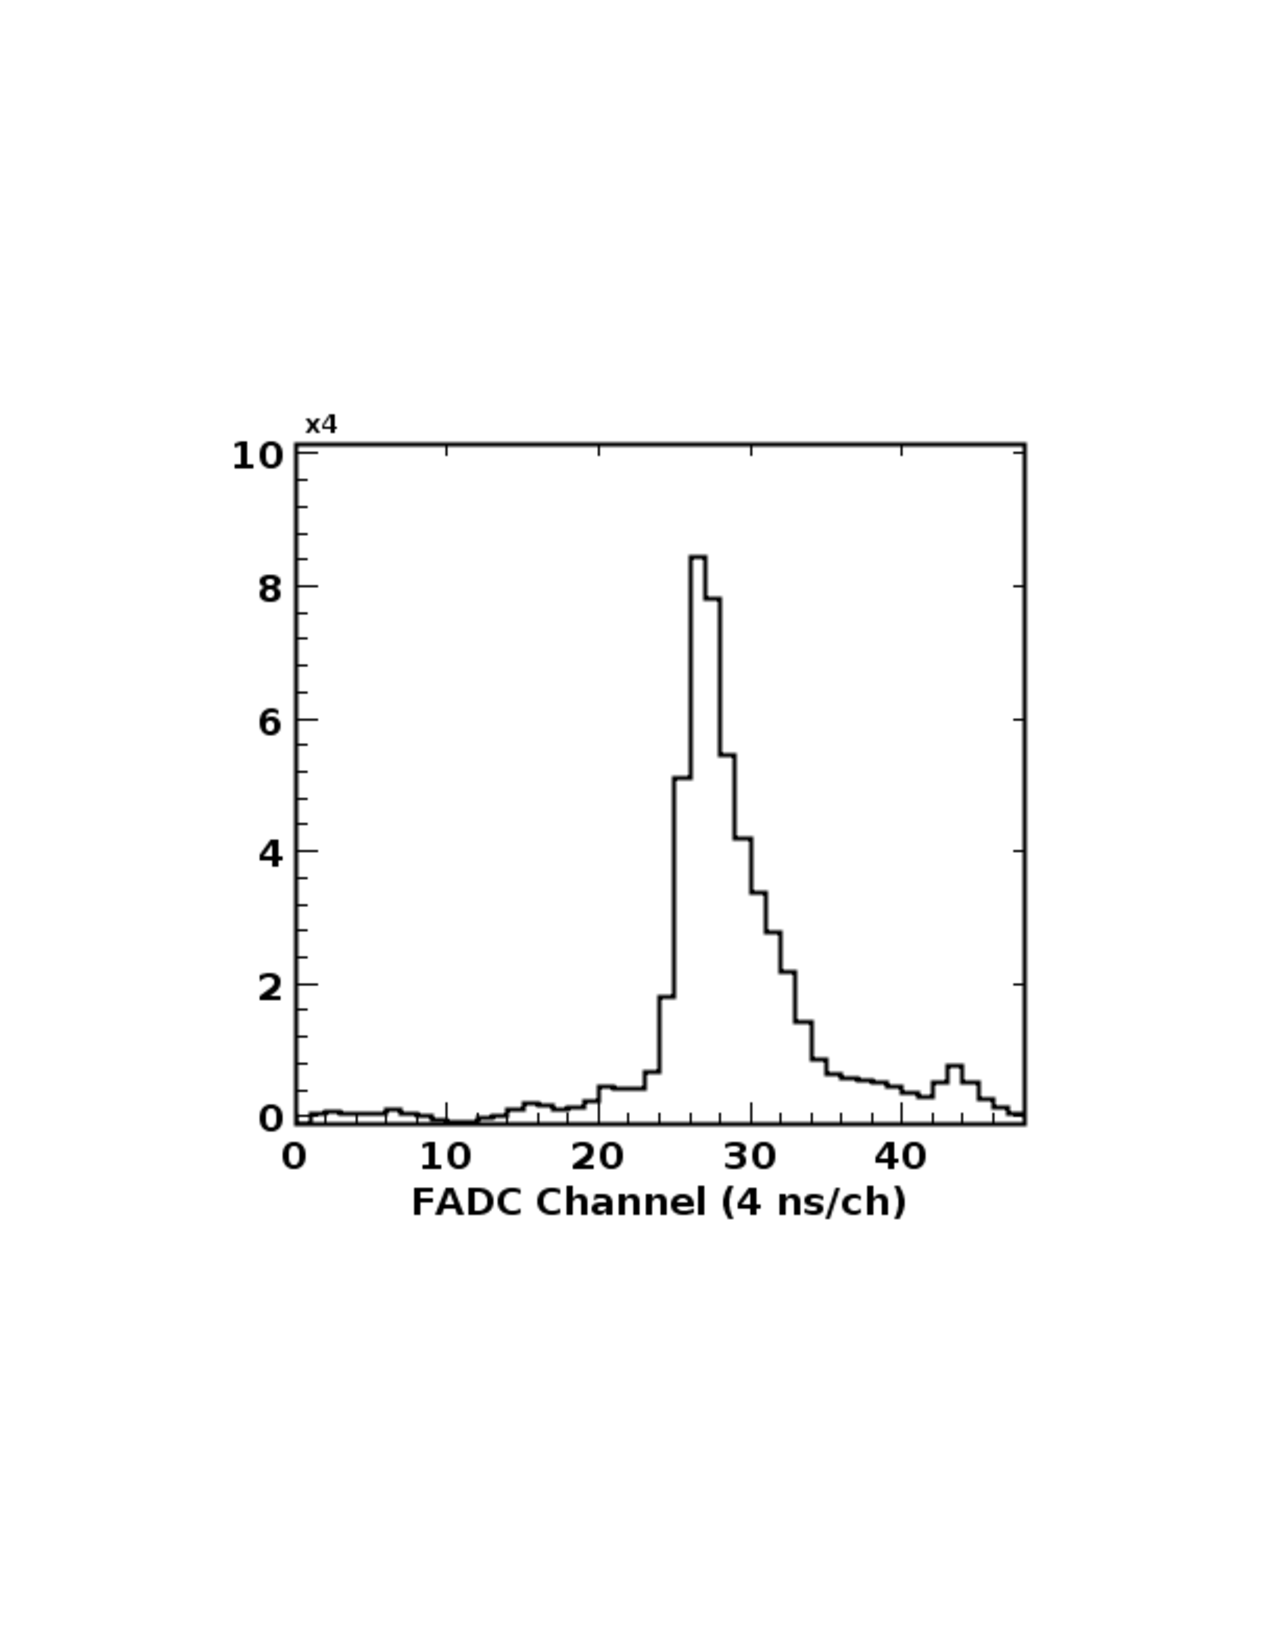
\includegraphics[width=0.65\textwidth,natwidth=610,natheight=642]{pics/ctof-fadc.pdf}}}
\end{picture} 
\caption{Average pedestal-subtracted FADC spectrum from a CTOF counter readout from beam data
with a 10.6~GeV electron beam incident upon a 5~cm liquid-hydrogen target with the JLab FADC250
module.}
\label{fadc-pulse}
\end{figure}
%%%%%%%%%%%%%%%%%%%%%%%%%%%%%%%%%%%%%%%%%%%%%%%%%%%%%%%%%

%%%%%%%%%%%%%%%%%%%%%%%%%%%%%%%%%%%%%%%%%%%%%%%%%%%%%%%%%
\begin{table}[htbp]
\begin{center}
\begin{tabular}{c|c} \hline
TDC Specs                           & ADC Specs \\ \hline
RMS resolution $\le$ 35~ps          & Sampling 250 MHz \\ \hline 
Resolution: 21~bit                  & Resolution: 12-bit \\ \hline
Inter-channel isolation $\le$ 3 LSB & Clock jitter 350~fs \\ \hline
Double-hit resolution 5~ns          & Data memory 8~$\mu$s \\ \hline    
Full-scale range 52~$\mu$s          & Trigger/Data latency 8~$\mu$s / 32~ns \\ \hline  
\multicolumn{2}{c}{Integral/Differential non-linearity} \\
$<$ 2.5 LSB / $<$ 3 LSB             & $\pm$0.5 LSB / $\pm$0.8 LSB \\ \hline
Inter-channel isolation $<$ 3 LSB   & SNR 56.8~dB @ 100~MHz input \\ \hline
\end{tabular}
\end{center}
\caption{The key performance specifications of the CTOF CAEN VX1290N pipeline TDCs and JLab 
FADC250 flash ADCs.}
\label{tdcadc-specs}
\end{table}
%%%%%%%%%%%%%%%%%%%%%%%%%%%%%%%%%%%%%%%%%%%%%%%%%%%%%%%%%

The PMT anode to splitter panel connections are made using LMR-195 cables, a low-loss variant 
of RG-58. LMR-195 is a coaxial cable with a 50~$\Omega$ characteristic impedance. The
upstream PMTs were connected to cable lengths of 15.9~m, 16.3~m, and 16.8~m and the 
downstream PMTs were connected to cable lengths of 20.7~m, 21.2~m, and 21.7~m. These cable 
lengths were required given the location of the CTOF electronics relative 
to the PMTs and were made as short as possible to minimize attenuation and dispersion of the 
anode signals. The three different signal cable lengths for the upstream and downstream PMTs 
are connected to neighboring PMTs in a repeating cyclical pattern. This layout was selected 
to mitigate the effects of possible counter-to-counter cross talk. The signal connections to the ADCs 
and TDCs were also set such that neighboring counters were not connected within the same module.
The cable connections from the splitters to the readout electronics used RG-316 cables of
1.5~m length. RG-316 is a low-loss variant of RG-174. RG-316 is a coaxial cable with a 
50~$\Omega$ characteristic impedance.

The PMTs for the CTOF counters typically operate at about 2000~V with negative polarity. The typical
dark current drawn by the PMTs on the assembled counters was $<20$~nA. The system is powered by a
single CAEN 527 high voltage mainframe outfitted with negative polarity 24-channel A1535N modules that
can supply up to 3.5~kV per channel with a maximum current of 3~mA. The power supply has a voltage ripple
specification of $<$20~mV peak-to-peak (typical). Each channel consumes less than 1~W during counter
operation. The typical supply currents per channel are 300~$\mu$A to 500~$\mu$A.

The mainframe is controlled remotely through the Hall~B Slow Controls system. A graphical user interface
using EPICS~\cite{epics} running on a UNIX system communicates with the mainframe via Ethernet. The
mainframe settings enable basic protection of the PMTs in terms of maximum voltage and current settings,
and channel ramp rates.

The high voltage cables for each PMT are fire-retardant RG-59 coaxial cables that run from the voltage
divider to a local disconnect high voltage (HV) distribution box located under the solenoid. There are two
48-channel HV distribution boxes for the CTOF. The output of each HV distribution box is a pair of 
35-ft-long multi-conductor cables, each containing 24-channels, with a Radiall connector to mate with the
HV A1535N board input connector. The multi-conductor high voltage cables employed each contain 30
conductors wrapped in Tefzel insulation, and outer wire shield and PVC insulation wrap. Each conductor
is 5-kV rated.

\section{CTOF Performance}
\label{sec:performance}

This section highlights the performance of the CTOF system both from the cosmic ray test stand
and in Hall~B during the first beam runs for CLAS12. The test stand timing performance is important
to understand to ensure that the performance specifications as detailed in Table~\ref{spec-table} are
met as the CTOF system is primarily responsible for the limits of the charged particle identification
separation for CLAS12 in the central direction. Full details on the bench test performance results for
the CTOF counters are provided in Ref.~\cite{dsc-cn2016-009}.

In this section the essential performance results from the bench testing studies in terms of the counter
photoelectron statistics and benchmark timing calibrations are presented. Then the nominal algorithms
are presented to provide details on how the in-beam CTOF timing was calibrated and the resolution
quantified. Finally, this section provides the current status of the particle identification capabilities
of the CTOF system in relation to the design specifications.

\subsection{Bench Measurements}
\label{sec:bench}

\subsubsection{Counter Photoelectron Statistics}
\label{sec:npe}

The primary approach to determine the number of photoelectrons at the photocathode of the PMTs
generated by minimum-ionizing particles in the scintillation bars employs the ratio of the integral of the
pulse for a minimum-ionizing particle to the integral of the pulse for a single photoelectron. For these
measurements we used the pulse integration feature of an Agilent Technologies~\cite{agilent-ref}
MSO-X 3034A 350~MHz (4 GSa/s) oscilloscope and averaged 1000 pulses. The minimum-ionizing particle
signals were analyzed connecting the scope to the PMT when mounted in position on the CTOF counter. For
the single photoelectron signal, we took data using just a bare PMT on the bench using the same gain setting.
For both measurements the oscilloscope threshold was adjusted appropriately. For the minimum-ionizing
peak analysis the threshold had to be set high enough ($>$200~mV) to eliminate tracks that did not pass
normally through the bar. For the single photoelectron peak the threshold had to be set low enough (1~mV)
to pick out the noise pulses that were the source of the PMT intrinsic dark current. This measurement
scheme yielded 200 photoelectrons per MeV of deposited energy at a gain of 1$\times$10$^6$, which
corresponds to $\sim$0.03~nC/MeV.

\subsubsection{Bench Time Resolution Performance}
\label{sec-bench}

The basic algorithm used on the test bench for the CTOF counters to determine the time resolution of
a given reference counter was to use incident cosmic ray muon tracks to compare the measured time
for the reference counter to the time measured by two other identical counters in a triplet counter
configuration (see Fig.~\ref{triplet}). For a triplet measurement, where the track passes through all
three counters with double-sided readout, six times are measured ($t_1 \to t_6$). Each time measurement
actually represents the difference between the discriminated PMT signal (TDC start) and the trigger time
(TDC stop from the six PMT coincidence). These timing measurements are then translated into three counter
hit times $t_{t,m,b} = \frac{1}{2}(t_{1,3,5} + t_{2,4,6})$.

%%%%%%%%%%%%%%%%%%%%%%%%%%%%%%%%%%%%%%%%%%%%%%%%%%%%%%%%%
\begin{figure}[htbp]
\vspace{4.2cm}
\begin{picture}(50,50) 
\put(70,5)
{\hbox{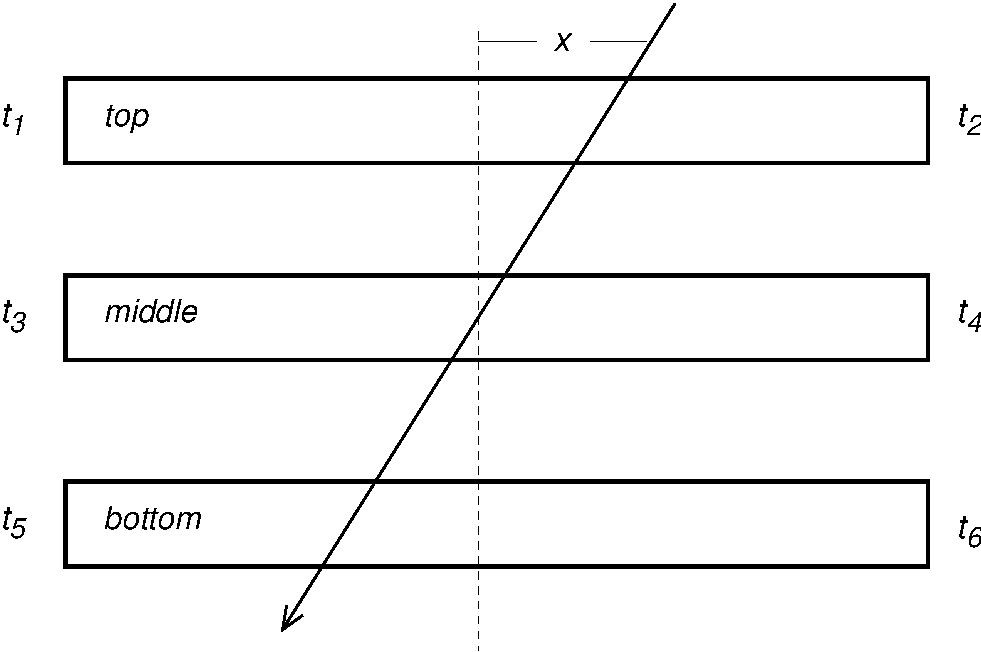
\includegraphics[width=0.80\textwidth,natwidth=610,natheight=642]{pics/triplet-alt.pdf}}}
\end{picture} 
\caption{Schematic representation of a triplet of counters (labeled top - $t$, middle - $m$, bottom - $b$)
with a muon track traversing the stack. The geometry of the triplet is configured such that the separation
between the top and middle counters matches that of the middle and bottom counters.}
\label{triplet}
\end{figure}
%%%%%%%%%%%%%%%%%%%%%%%%%%%%%%%%%%%%%%%%%%%%%%%%%%%%%%%%%

For incident tracks that pass fully through each counter of the triplet with measured times $t_t$, $t_m$,
and $t_b$, we can define a time residual $t_r = t_m - \frac{1}{2}(t_t + t_b)$, where we should expect that
the time $t_m$ of the middle scintillator hit should be the average of the measured times $t_t$ and $t_b$
for the top and bottom scintillator hits, respectively. Thus the measured residual $t_r$ should nominally be 0.
However, due to the smearing of the measured times $t_t$, $t_m$, and $t_b$ due to the finite time resolution
of the measurements, the residual time $t_r$ will also be smeared. While we still expect the mean of $t_r$ to
be zero, the width of the $t_r$ distribution can be used to determine the average time resolution of each
counter in the triplet. (For the outer counters in the triplet, the definition of the time residual must be slightly
modified to account for the small path length difference between the reference counter and the other two
counters.)

The average time resolution of each counter is computed from the variance $\delta t_r$ in the measured time
residual $t_r$. Assuming the average time resolution for each PMT in the triplet ($\Delta t_i$, $i = 1 \to 6$)
is identical and taking into account that each counter is readout using two PMTs, we can write the final expression
for the average counter timing resolution as:

\begin{equation}
\label{sig-counter}
\sigma_{counter} = \frac{2}{\sqrt{6}} \delta t_r.
\end{equation}

\noindent
Thus a measure of the width ($\sigma$) of the time residual distribution provides a measure of the
average resolution of each counter in the triplet. 

\subsubsection{Bench Measurement Counter Timing Resolutions}
\label{bench-tres}

Fig.~\ref{res-avg} shows the average timing resolution measured for each CTOF counter using the
triplet counter configuration. This analysis included a minimum ADC cut to remove events with low
photon statistics that did not pass through the full width of the counter and also a coordinate cut of
$\pm$10~cm about the center of the scintillation bar. Here the average counter timing resolution is
roughly 70~ps. The resolution on average is slightly worse for the top and bottom counters of each
cart due to the uncertainties in the path length corrections discussed in Section~\ref{sec-bench}.
Given the discussion of the time resolution measurement limitations in Section~\ref{res-limitations},
these results are quite encouraging compared to the design specifications.

%%%%%%%%%%%%%%%%%%%%%%%%%%%%%%%%%%%%%%%%%%%%%%%%%%%%%%%%%
\begin{figure}[htbp]
\vspace{5.2cm}
\begin{picture}(50,50) 
\put(57,-65)
{\hbox{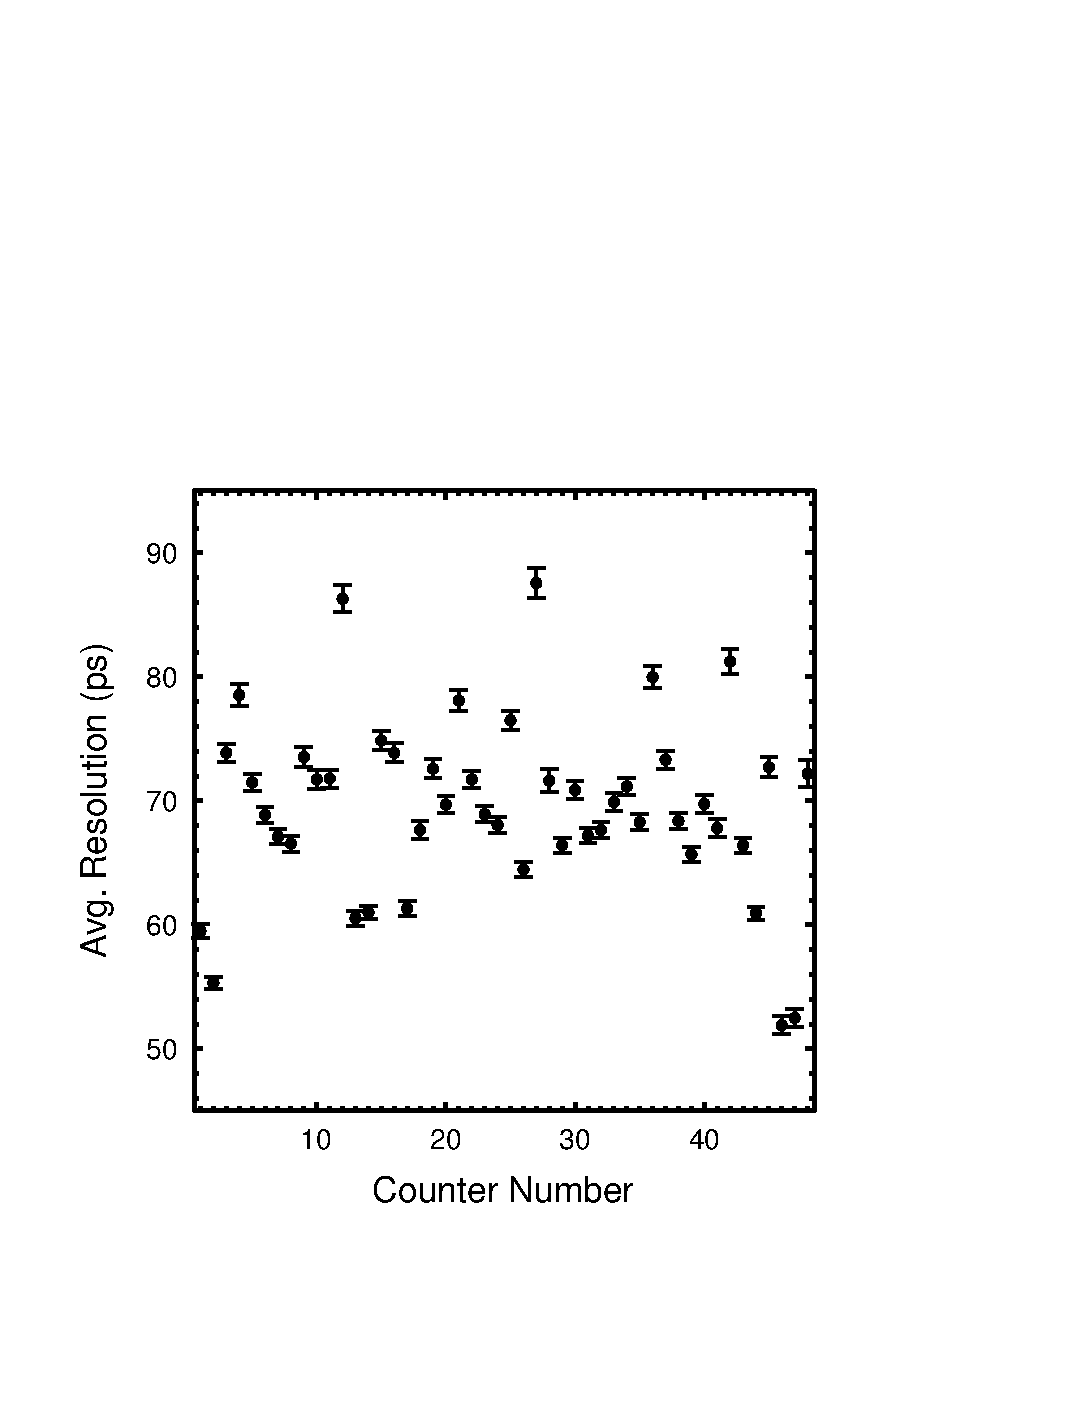
\includegraphics[width=0.90\textwidth,natwidth=610,natheight=642]{pics/res-comp35.pdf}}}
\end{picture} 
\caption{Measured average CTOF counter resolution with a cut on the measured ADC values and a cut on
the measured hit coordinates to select events going through the middle of the counter. The vertical line
separates the low-pitch angle counters (\#1 to \#24) from the high-pitch angle counters (\#25 to \#48).}
\label{res-avg}
\end{figure}
%%%%%%%%%%%%%%%%%%%%%%%%%%%%%%%%%%%%%%%%%%%%%%%%%%%%%%%%%

The CTOF counter time resolutions were studied vs. three independent variables: track coordinate,
ADC geometric mean, and track angle. Table~\ref{res-studies} shows details on the variable 
ranges and bin sizes used for these studies. The bin sizes were selected to achieve reasonable 
statistical precision in the measurements given the limited statistics for the week-long data run.

%%%%%%%%%%%%%%%%%%%%%%%%%%%%%%%%%%%%%%%%%%%%%%%%%%%%%%%%%
\begin{table}[htpb]
\begin{center}
\begin{tabular} {|c|c|c|c|c|} \hline
Quantity           & $N_{bins}$ & Lower Limit & Upper Limit & Bin Size \\ \hline
Track Coordinate   & 16 & -40 cm      & 40 cm      & 5~cm \\ \hline
ADC Geometric Mean & 16 & 1250        & 6050       & 300 channels \\ \hline
Track Angle        & 16 & -45$^\circ$ & 45$^\circ$ & 5.625$^\circ$ \\ \hline
\end{tabular}
\end{center}
\caption{Details on the limits and bin sizes selected for the counter timing resolution studies vs.
track coordinate, ADC geometric mean, and track angle.}
\label{res-studies}
\end{table}
%%%%%%%%%%%%%%%%%%%%%%%%%%%%%%%%%%%%%%%%%%%%%%%%%%%%%%%%%

Fig~\ref{res-ctof2} shows the average resolution for a representative CTOF counter as a function
of hit coordinate, ADC value, and track incidence angle. The resolution is optimal about the center of
the counter and gets worse near the ends where one PMT receives its minimum light due to attenuation
length effects. The resolution is reasonably flat over the ADC range corresponding to muons more or
less normally incident upon the counters (channel 2000 for these studies). There is a slight improvement
with higher ADC values as more light reaches the PMTs. As the resolution is proportional to photo-statistics, 
the larger the energy deposited the better the timing resolution. The resolution improves with increasing
angle due to a correspondingly longer path through the scintillation material that results in increased
photo-statistics.

%%%%%%%%%%%%%%%%%%%%%%%%%%%%%%%%%%%%%%%%%%%%%%%%%%%%%%%%%
\begin{figure}[htbp]
\vspace{3.7cm}
\begin{picture}(50,50) 
\put(15,-200)
{\hbox{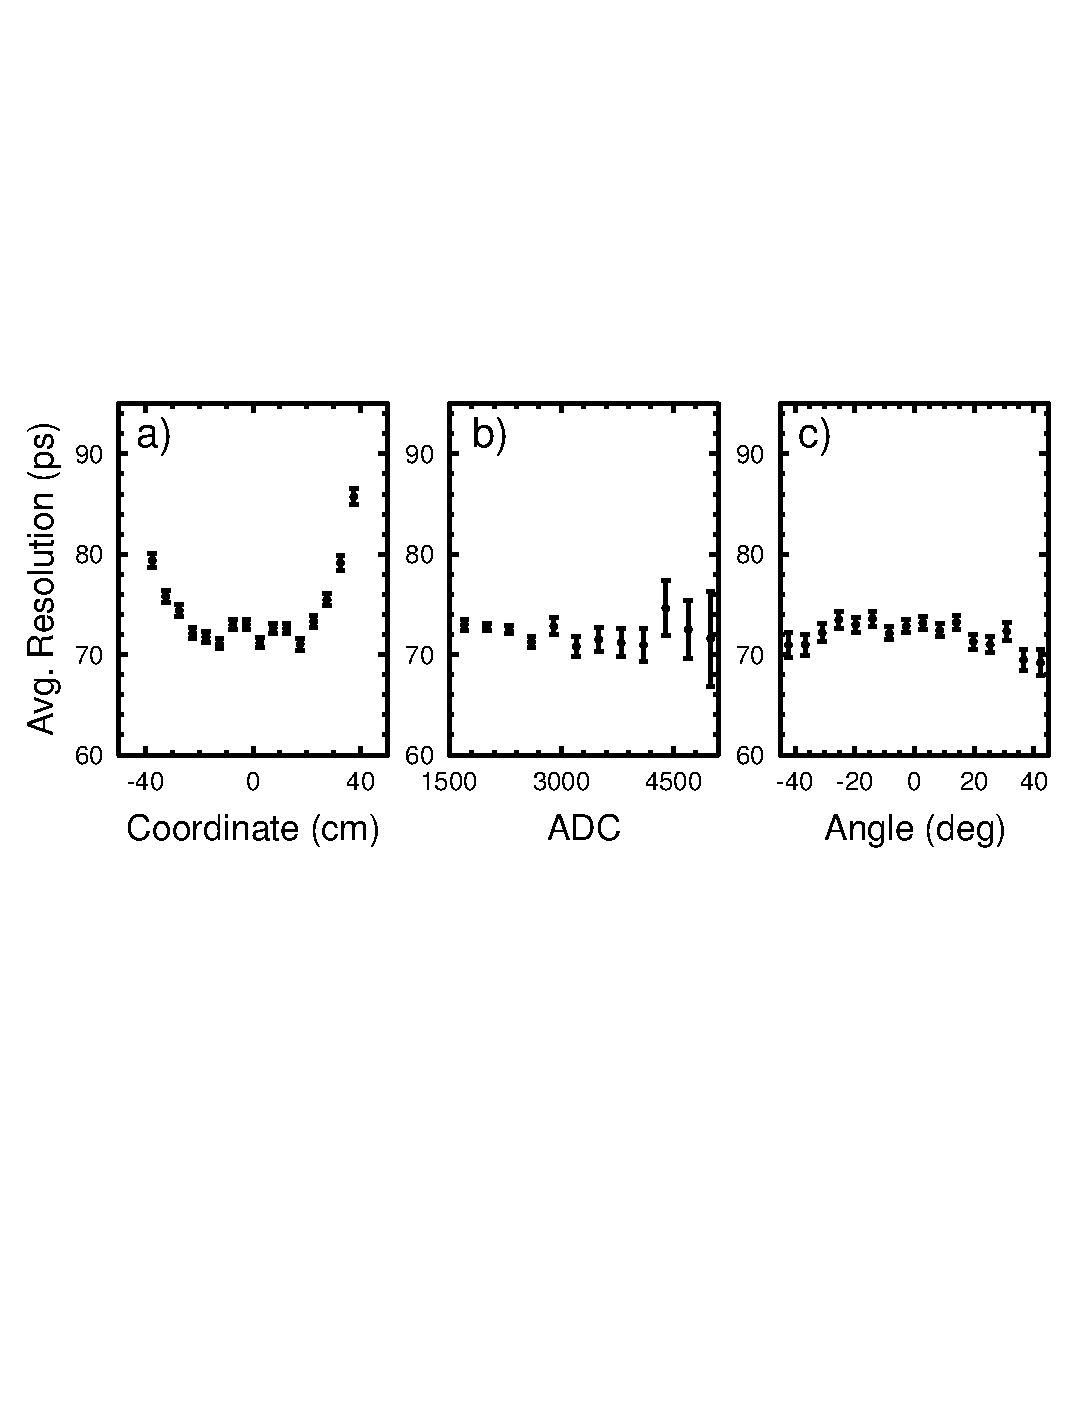
\includegraphics[width=1.1\textwidth,natwidth=610,natheight=642]{pics/res-dep.pdf}}}
\end{picture} 
\caption{Dependence of the counter time resolution for a representative counter on a). the
coordinate of the reference counter, b). the average reference counter ADC value, and c). the
angle of incidence of the track.}
\label{res-ctof2}
\end{figure}
%%%%%%%%%%%%%%%%%%%%%%%%%%%%%%%%%%%%%%%%%%%%%%%%%%%%%%%%%

One final note to mention here with regard to the bench test time counter resolution measurements 
is that a series of studies were carried out replacing the constant fraction discriminators (CFDs) 
with leading edge discriminators (LEDs). The timing resolution results using LED readout including
appropriate off-line time-walk corrections were consistent with those using the CFDs that do not require
the time-walk corrections. These results are detailed in a separate report~\cite{twalk}.

\subsubsection{Limitations to Bench Measurements}
\label{res-limitations}

There are two factors involved in the bench test studies that limited the accuracy of the measured
CTOF counter time resolutions. The first arose from the extremely low data rate for each triplet 
of counters ($< 0.1$~Hz) due to the narrow counter width and the counter-to-counter separation of 
$\sim$21.6~cm. Data runs of $\sim$1~week were necessary to collect sufficient statistics to 
determine the counter resolutions. Due to the inherent calibration drifts over this time that 
could not be tracked precisely, the measured counter time resolutions were smeared. The second
factor arose due to the counter-to-counter alignment within the carts was only at the level of
$\pm$0.64~cm. This scale was set by the fairly crude design of the carts and the counter supports,
which were mainly intended for counter assembly, wrapping, and storage. With counter-to-counter
separations of $\sim$21.6~cm, the inaccuracies of the alignment were such that the residual centroids
were correlated with the hit coordinates, which again smeared the counter time resolutions. The
contributions of both factors smeared the measured time resolutions by 10\% to 20\%. 

\subsection{CTOF Beam-Data Calibrations}

In the nominal data taking mode for CLAS12, whenever the CTOF is involved in an event that triggers the
spectrometer, the ADCs and TDCs for all PMTs with a signal above the discriminator threshold are recorded.
For the FADCs, the charge of the pulse is integrated over the extent of the pulse region and the pedestal is
subtracted event by event as discussed in Section~\ref{sec-elec}. For the TDCs the time recorded is relative
to the trigger. To determine the flight time of the charged track from the target to the CTOF, the TDC time
must be compared to the time of the accelerator radio frequency (RF) pulse relative to the trigger.  The RF
signal from the accelerator has a period an integer multiple of 2.004~ns. The RF bunch length itself corresponds
to a few picoseconds. Although the timing signals are very accurate (with a resolution of $<$20~ps), the
determination of which beam bunch produced a given interaction must be determined by the experiment.

The full energy and timing calibration of the each of the CTOF counters involves a number of discrete steps. The
calibration constants for each run are stored in the CLAS12 calibration database. The calibrations are monitored
for each data run (which lasts typically for 2~hrs) and redone only when there are shifts in the response outside
of established ranges (which are typically 5\%). The steps to the CTOF calibration are carried out in a particular
as detailed in Ref.~\cite{ctof-calib} and highlighted below.

\begin{enumerate}
\item ADC Calibration: Determine the ADC channel to energy deposition calibration factor for each counter
using minimum-ionizing events. See Section~\ref{gain-matching}.

\item Upstream/downstream PMT time offsets: This time offset accounts for the difference in the time
recorded between the upstream and downstream PMTs in a given counter due mainly to the different
signal cable lengths used for the connection to the readout electronics. These time offsets are determined
from the centroid of the difference between the upstream/downstream TDC time difference and the
computed track hit coordinated divided by the effective speed of light in the counter. 

\item Attenuation Length Calibration: This property of the counter quantifies the light absorption length and
is determined by relating the measured ADC as a function of hit coordinate along the bar. See
Section~\ref{sec:attlen}.

\item Effective Velocity Calibration: Determine the effective speed of light propagation along the counter. See
Section~\ref{sec:veff}.

\item Counter-to-Counter Time Offset Calibration: In order to measure the absolute flight time of a charged
particle from the target to the CTOF counter and to be able to reconstruct exclusive events when hits are
associated with multiple CTOF counters, the relative time offsets of each counter relative to all of the other
counters in the system need to be determined. This is done in two steps. The first step is to align each track
to the RF time, a step that amounts to a precision time alignment in bins of the TDC LSB. The second step is a
coarse alignment of each counter time in bins of the RF period $T_{RF}$. See Section~\ref{sec-talign}. During
this step the effective counter timing resolutions are extracted (see Section~\ref{tres-beam}).

\item TDC Calibration: After calibrating the integral non-linearities of each TDC channel in the system (see
Section~\ref{sec-elec}), the TDC channel to time calibration is completed using beam events. See
Section~\ref{sec-tdccal}.

\end{enumerate}

\subsubsection{Gain Matching}
\label{gain-matching}

One of the purposes of gain-matching the CTOF PMTs is to equalize the detector response to tracks that
cross the CTOF barrel such that two counters are involved. This is a necessary procedure because each
counter must contribute equally to the trigger for a common-threshold discriminator level. Gain matching
so that the minimum-ionizing particle peak appears in the same ADC channel for all counters also allows for
easier data monitoring during online and offline analysis.

The CTOF PMT high voltage settings were determined using calibration runs employing minimum-ionizing
tracks. These minimum-ionizing tracks deposit roughly 6~MeV as they pass through the 3~cm thick CTOF
scintillation bars, as $dE/d\rho x = 1.956$~MeV/g/cm$^2$ for minimum-ionizing particles. The initial high
voltage settings were based on runs using cosmic ray muons with the solenoid at zero field with the readout
based on a trigger that required tracks to cross the barrel to select tracks approximately normal to the
face of the CTOF counters. During production data taking, these calibrations are carried out using
minimum-ionizing tracks from beam data coming from the target. In this case the charge information is
scaled by a path length correction given by $t/P$, where $t$ is the counter thickness and $P$ is the
path-length of the track in the counter as determined by extrapolation of the track beyond the central
tracker to the location of the CTOF counter.

The energy deposited in the scintillation bars follows a Landau distribution for the minimum-ionizing tracks.
The energy deposited is recorded by the ADCs, which show a peak above pedestal for the tracks. Tracks
that do not pass through the full counter thickness and non-minimum-ionizing tracks give rise to a background
beneath the Landau peak.

For the HV calibrations, to avoid issues with the attenuation of light for tracks that pass near the ends of
the bars and to avoid issues with unbalanced light entering the upstream and downstream PMTs, we combine
the pedestal-subtracted ADC information from the upstream and downstream PMTs to produce an average
ADC spectrum for the counter through the quantity known as the ADC geometric mean given by:

\begin{equation}
\label{adc}
\overline{ADC} = \sqrt{ (ADC - PED)_U \cdot (ADC - PED)_D}.
\end{equation}

\noindent
Fig.~\ref{gmean} shows the geometric mean spectrum for one representative CTOF counter using beam data.

Given the finite dynamic range of the ADC, we have chosen to position the minimum-ionizing muon peak in a
particular ADC channel that is selected so that it is safely above the pedestal, but leaves sufficient range
for the more highly ionizing charged tracks of our typical physics events. To minimize PMT aging effects that
result in loss of PMT gain with time correlated with the total charge collected at the first dynode of the
accelerating structure, the PMT gains are set as low as possible.

%%%%%%%%%%%%%%%%%%%%%%%%%%%%%%%%%%%%%%%%%%%%%%%%%%%%%%%%%
\begin{figure}[htbp]
\vspace{4.2cm}
\begin{picture}(30,50) 
\put(105,-35)
{\hbox{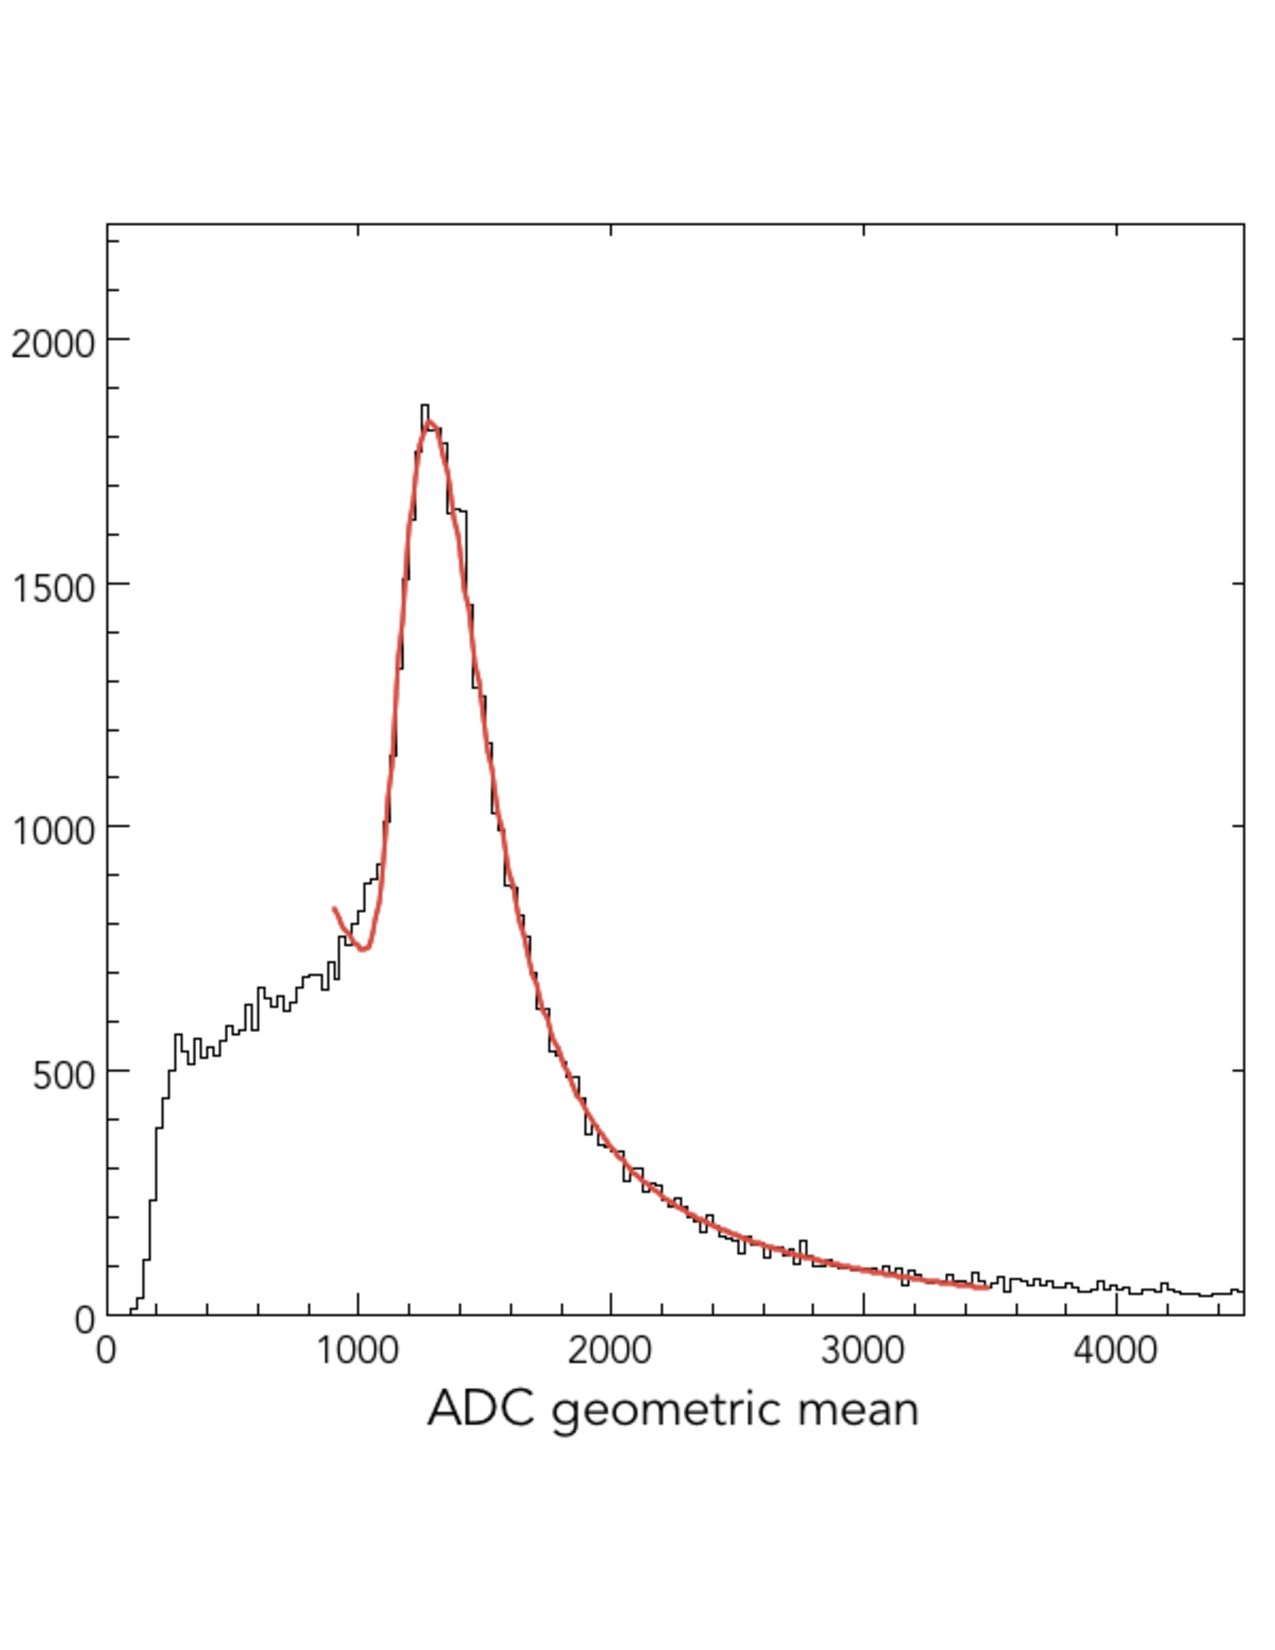
\includegraphics[width=0.45\textwidth,natwidth=610,natheight=642]{pics/gmean.pdf}}}
\end{picture} 
\caption{(Color Online) Geometric ADC mean for one representative CTOF counter from beam data
in CLAS12. The events recorded in the ADC spectrum have been pedestal subtracted. The red curve
is the fit function that includes a Landau shape for the peak and an exponential for the background.}
\label{gmean}
\end{figure}
%%%%%%%%%%%%%%%%%%%%%%%%%%%%%%%%%%%%%%%%%%%%%%%%%%%%%%%%%

The PMT gains depend exponentially on the applied voltage. Expressed in a slightly different way, we 
can relate the PMT gain $G_1$ at a given voltage $V_1$ to the gain $G_2$ at a different voltage $V_2$ 
via:

\begin{equation}
\label{power-law}
\frac{G_1}{G_2} = \left( \frac{V_1}{V_2} \right) ^\alpha.
\end{equation}

\noindent
This is a basic power law form with $\alpha$ representing the power law factor. Rewriting
Eq.(\ref{power-law}) in a slightly different form, we have:

\begin{equation}
\label{delta}
\frac{\Delta G}{G} = \alpha \frac{\Delta V}{V}.
\end{equation}

It is this expression that is the basis for relating the position of the muon peak in the $\overline{ADC}$
spectrum (see Eq.(\ref{adc})) to the PMT HV setting. The gain-matching procedure then amounts to
adjusting the HV settings of all PMTs to the values required to position the muon peak for each counter
in the desired ADC location. At the same time the algorithm uses the individual upstream and downstream
PMT ADC spectra for a given counter to ensure that these PMT gains are balanced.

The iterative process to determine the final set of PMT HV values typically converges in 1 to 2 data runs.
For initial operation of the PMTs we have chose to center the muon peak in the $\overline{ADC}$ spectrum
for each counter in channel 900. At the typical PMT voltage settings of $-1500 \to -2000$~V, the HV supply
currents for each channel are in the range from 300~$\mu$A to 500~$\mu$A. 

The determination of the power law factor $\alpha$ in Eq.(\ref{power-law}) is important in order for the
HV calibrations to converge quickly. This factor can be determined directly from the data. For this purpose,
two data runs were acquired with different HV settings for the PMTs. After determining the locations of the
muon peaks from the ADC spectrum fits, Eq.(\ref{delta}) was used to solve for $\alpha$ for all PMTs. The
average value from the data was determined to be $\alpha$=4 as shown in Fig.~\ref{alpha-data}.

%%%%%%%%%%%%%%%%%%%%%%%%%%%%%%%%%%%%%%%%%%%%%%%%%%%%%%%%%
\begin{figure}[htbp]
\vspace{4.0cm}
\begin{picture}(50,50) 
\put(15,-90)
{\hbox{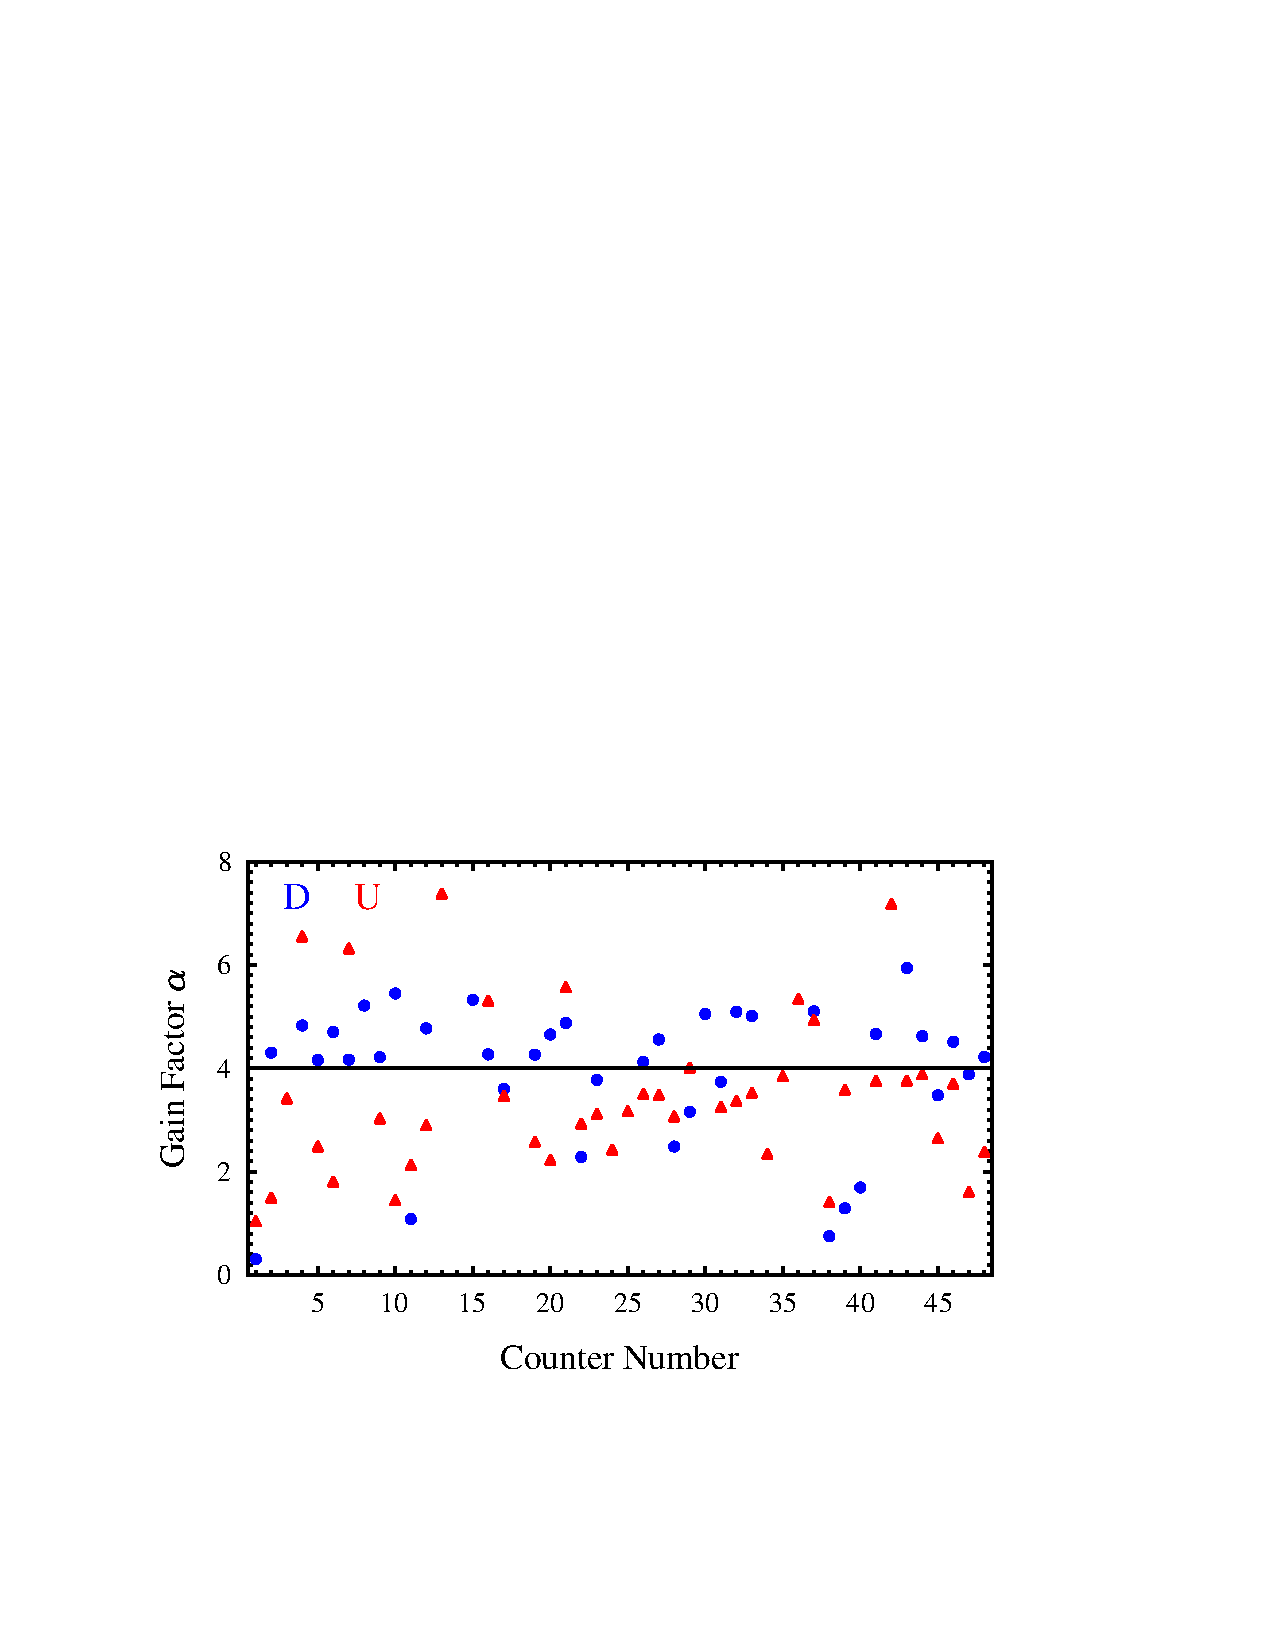
\includegraphics[width=1.00\textwidth,natwidth=610,natheight=642]{pics/alpha1.pdf}}}
\end{picture} 
\caption{(Color Online) Data showing the measurements of the power law factor $\alpha$ for each
CTOF upstream PMT (red triangles) and downstream PMT (blue circles). The average values of $\alpha$
for the CTOF PMTs is 4.}
\label{alpha-data}
\end{figure}
%%%%%%%%%%%%%%%%%%%%%%%%%%%%%%%%%%%%%%%%%%%%%%%%%%%%%%%%%

The energy loss in a counter for a passing charged particle track is determined after the
minimum-ionizing peak centroids are aligned. The computed energy loss in each counter is
computed from each PMT as:

\begin{equation}
E_{U,D} = ADC_{U,D} \cdot \left [ \frac{\left( \frac{dE}{dx} \right)_{MIP} \cdot t}{ADC_{MIP}}\right ]
\exp\left(\frac{d_{U,D}}{\lambda}\right),
\end{equation}

\noindent
where $ADC_{MIP}$ is the centroid of the minimum-ionizing peak in the geometric mean distribution,
$\left( \frac{dE}{dx} \right)_{MIP}$ is the energy loss for minimum-ionizing particles in the scintillation
bars (1.956~MeV/cm), $t$ is the counter thickness, $d$ is the distance along the bar from the track hit
position to the PMT, and $\lambda$ is the counter attenuation length. The energy loss used in the event
reconstruction is the mean of the separate $E_{U,D}$ measures.

Fig.~\ref{ctof-dedx} shows the reconstructed energy loss normalized by the track path length summed
over all counters from a data run with a 10.6~GeV electron incident upon a liquid-hydrogen target. The
data allow the separation of minimum-ionizing particles from more heavy ionizing particles. The
minimum-ionizing particles lose a constant energy as a function of path length. The heavily ionizing particles
have energy loss that increases linearly with distance at low momentum until they can pass through the
counter. At that point their energy loss follows the Bethe-Bloch formula.

%%%%%%%%%%%%%%%%%%%%%%%%%%%%%%%%%%%%%%%%%%%%%%%%%%%%%%%%%
\begin{figure}[htbp]
\vspace{5.0cm}
\begin{picture}(50,50) 
\put(20,230)
{\hbox{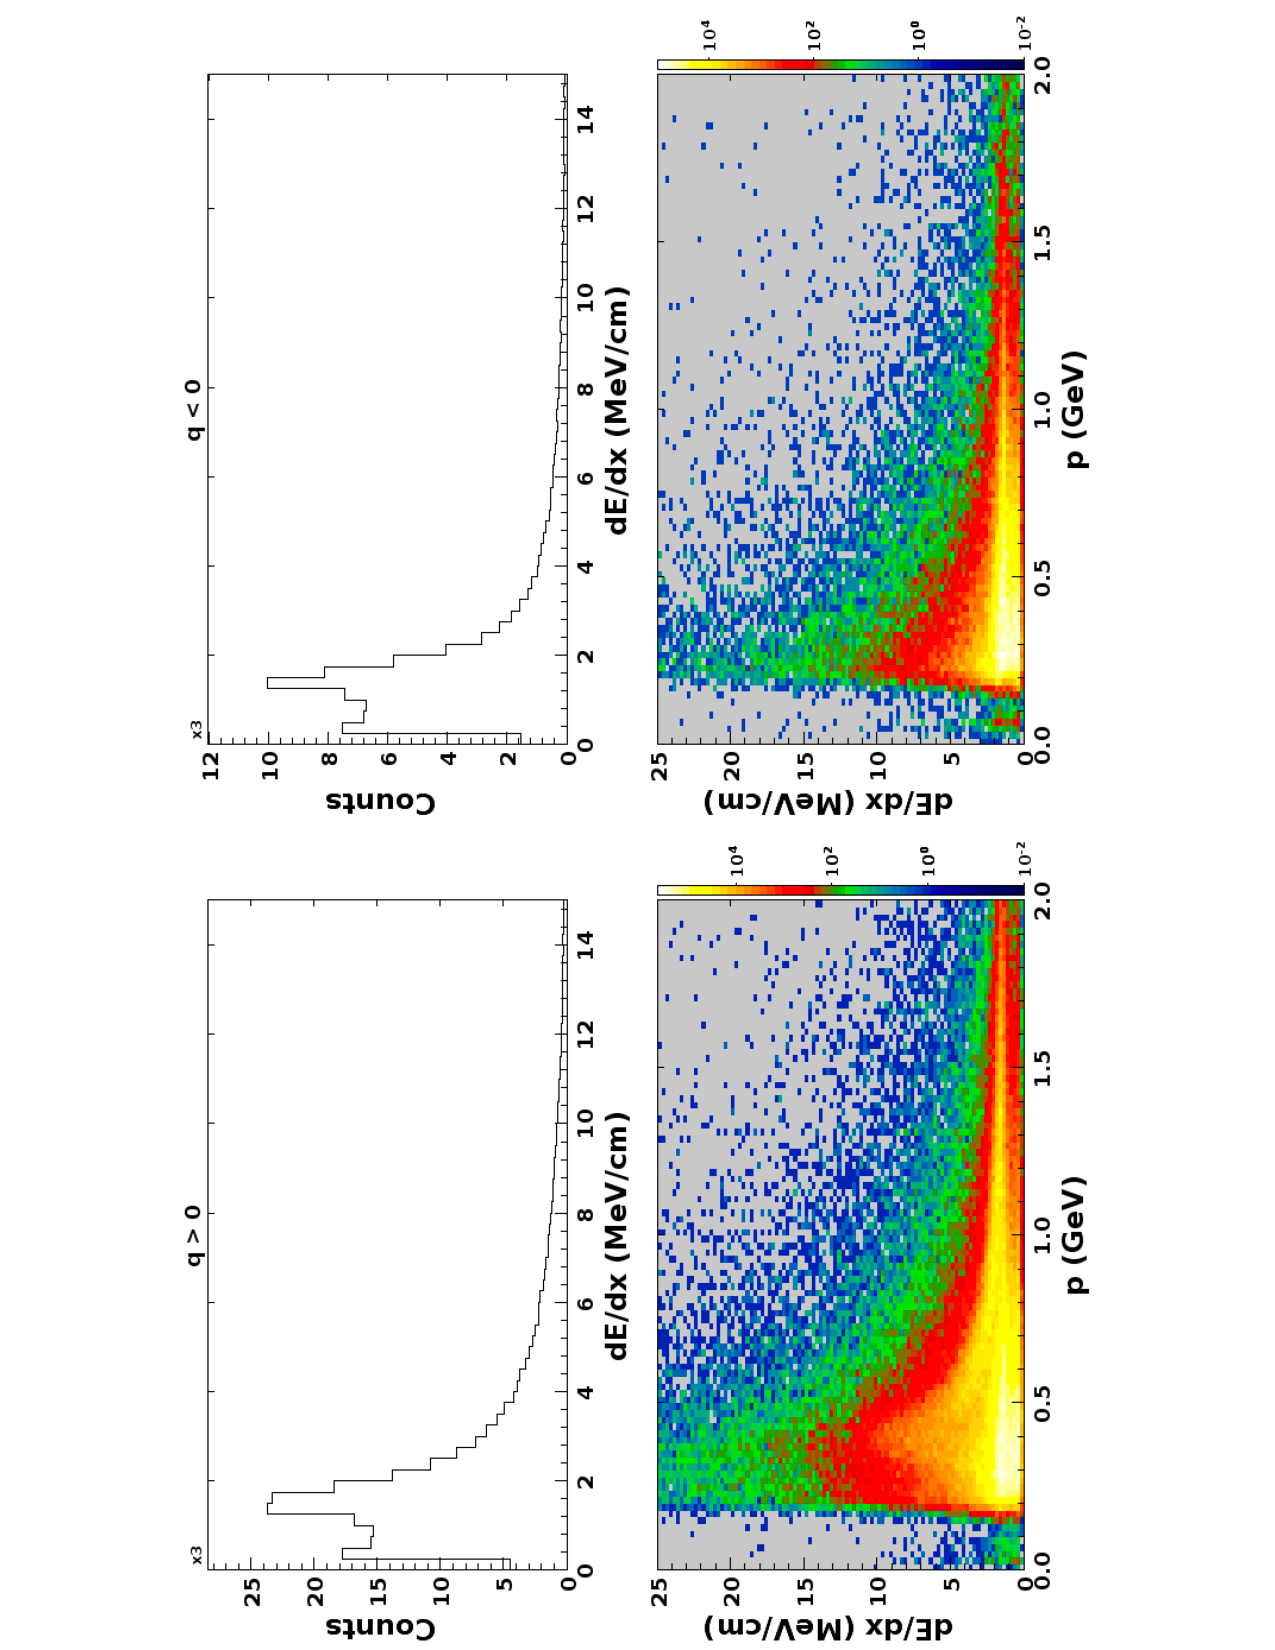
\includegraphics[width=0.7\textwidth,natwidth=610,natheight=642,angle=-90]
{pics/ctof-dedx.pdf}}}
\end{picture} 
\caption{(Color Online) Measured CTOF counter energy loss summed over all counters for positively
charged particles (left column) and negatively charged particles (right column) from 10.6~GeV
electrons incident on a liquid-hydrogen target normalized by the extrapolated path length from the
projection of the central track through the CTOF barrel. These $dE/dx$ (MeV/cm) plots show
separation of minimum-ionizing particles from more heavily ionizing particles. The top row of plots show
the measured $dE/dx$ and the bottom row of plots show $dE/dx$ vs. track momentum (GeV).}
\label{ctof-dedx}
\end{figure}
%%%%%%%%%%%%%%%%%%%%%%%%%%%%%%%%%%%%%%%%%%%%%%%%%%%%%%%%

\subsubsection{Attenuation Length Measurements}
\label{sec:attlen}

The attenuation length of the scintillation bars represents the distance $\lambda$ into the 
material where the probability that the photon has been absorbed is $1/e$. For the scintillation 
bars, as more collected light translates into better timing resolution, it is important for the 
attenuation length to be as long as possible. The general design goal was that the attenuation length 
be on the order of the overall length of the bars.

For EJ-200, this bulk attenuation length is reported by the manufacturer as 380~cm
\cite{scint-spec}. The practical attenuation length of the scintillation material turns out to 
be about half the bulk attenuation length. The coupling of the CTOF scintillation bars to the 
Acrylic light guides reduces the measured counter practical attenuation length by another 
$\sim$35\% to 50\% (corresponding to $e^{-L_{LG}/\lambda_A}$, where $L_{LG}$ is the light guide 
length and $\lambda_A$=2.3~m (see Section~\ref{optical-tests})).

The measured ADC values for each PMT can be written in terms of the attenuation length as:

\begin{equation}
\label{al-adc}
ADC_{U,D} = A_0^{U,D} e^{\pm x/\lambda},
\end{equation}

\noindent
where $A_0^U$ and $A_0^D$ are constants and $\lambda$ is the counter attenuation length. Then,

\begin{equation}
\label{linear}
\log \left( \frac{(ADC-PED)_U}{(ADC-PED)_D} \right ) = C + \frac{2x}{\lambda}, 
\end{equation}

\noindent
and a linear fit of the ADC log ratio vs. coordinate $x$ is used to extract the effective counter attenuation
length. Here the hit coordinate along the counter is determined using the measured TDC hit times $t_U$
and $t_D$ from:

\begin{equation}
\label{coor}
x = (t_U - t_D) \cdot \frac{v_{eff}}{2},
\end{equation}

\noindent
where $v_{eff}$ is the effective velocity of light in the scintillation counter. Note that the PMT transit
time and signal cable propagation times are taken out to center the coordinate distribution about zero.
Fig.~\ref{atten-len1} shows the measured average attenuation lengths for the CTOF counters. The 
average attenuation length is found to be 140~cm in accord with expectations. 

%%%%%%%%%%%%%%%%%%%%%%%%%%%%%%%%%%%%%%%%%%%%%%%%%%%%%%%%%
\begin{figure}[htbp]
\vspace{3.6cm}
\begin{picture}(30,50) 
\put(55,-200)
{\hbox{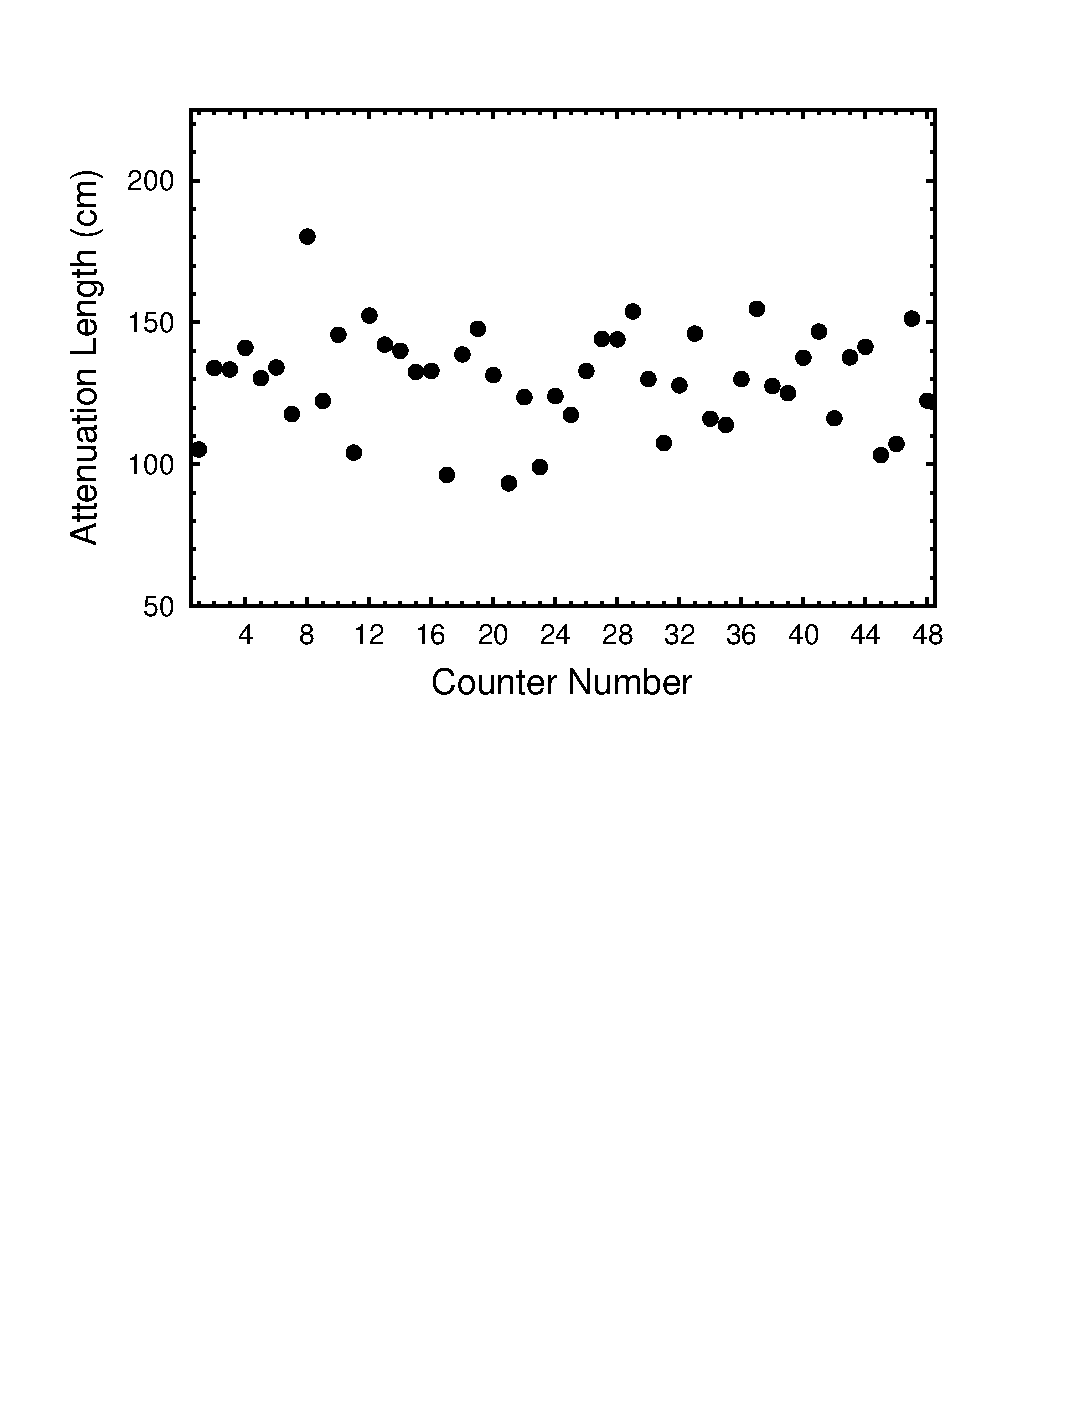
\includegraphics[width=0.85\textwidth,natwidth=610,natheight=642]{pics/atten.pdf}}}
\end{picture} 
\caption{Counter attenuation lengths (cm) vs. counter number determined from beam data.}
\label{atten-len1}
\end{figure}
%%%%%%%%%%%%%%%%%%%%%%%%%%%%%%%%%%%%%%%%%%%%%%%%%%%%%%%%%

\subsubsection{Effective Velocity Determination}
\label{sec:veff}

The effective velocity of light in each counter employs a calculation based comparing the reconstructed
coordinate information along the scintillation bar from the timing information and from the track hit
coordinate determined from extrapolation of the track beyond the central vertex tracker to the location
of the CTOF counters. Fig.~\ref{veff} shows the measured effective velocity for each CTOF counter using
data with a 10.6~GeV electron beam incident on a liquid-hydrogen target. 

%%%%%%%%%%%%%%%%%%%%%%%%%%%%%%%%%%%%%%%%%%%%%%%%%%%%%%%%%
\begin{figure}[htbp]
\vspace{3.6cm}
\begin{picture}(30,50) 
\put(55,-200)
{\hbox{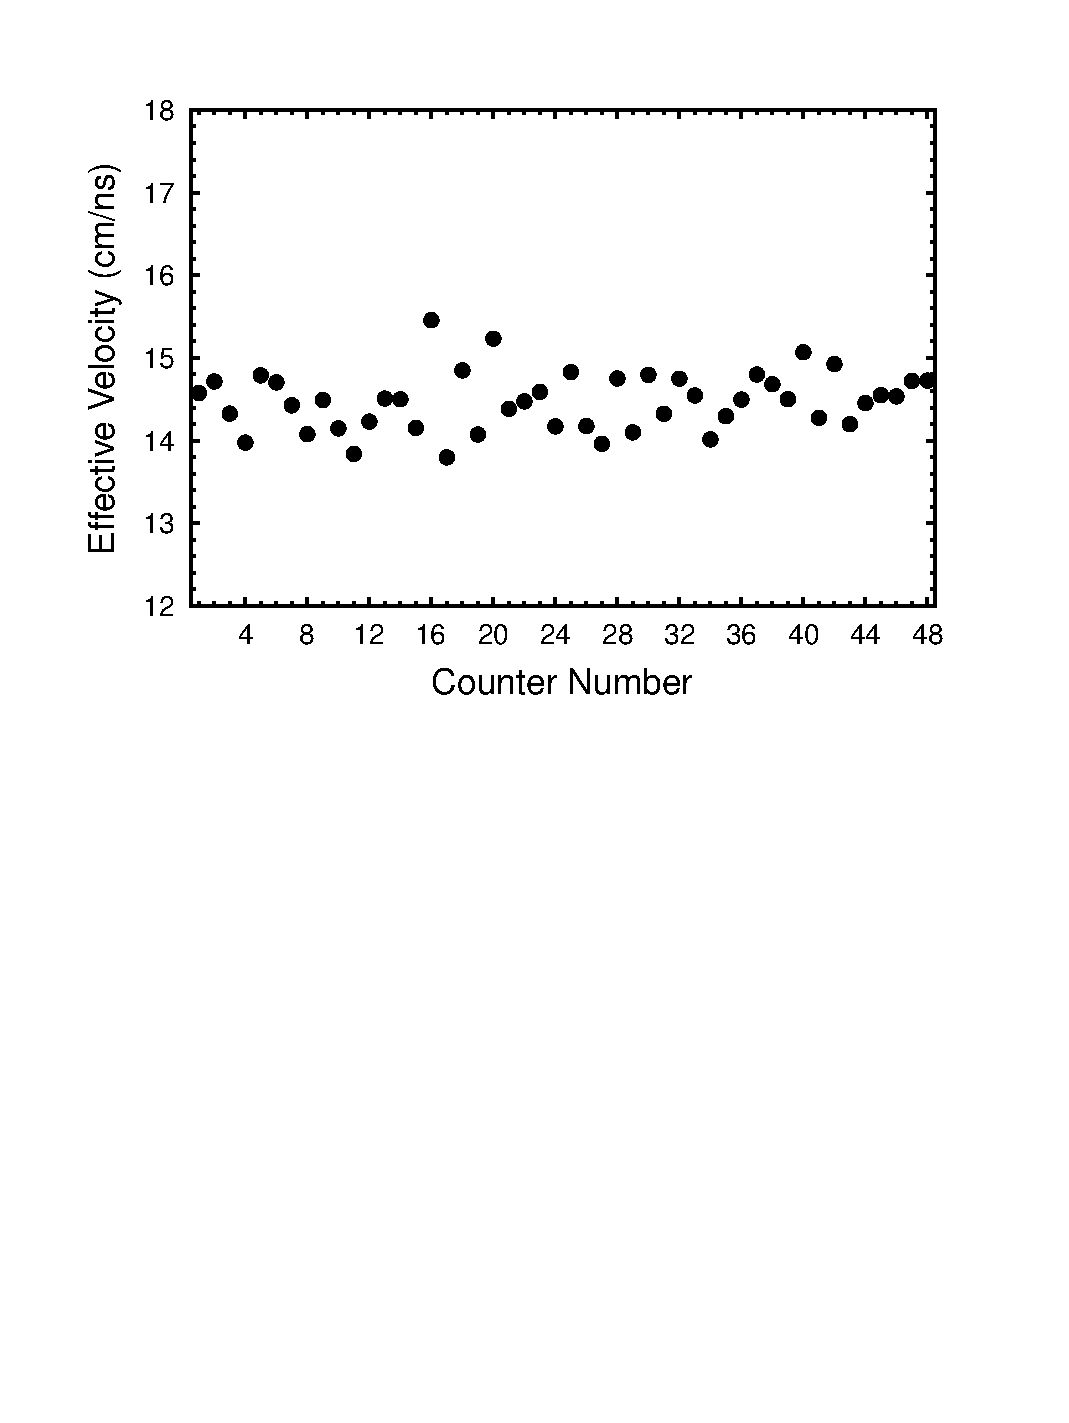
\includegraphics[width=0.85\textwidth,natwidth=610,natheight=642]{pics/veff.pdf}}}
\end{picture} 
\caption{Counter effective velocities (cm/ns) vs. counter number determined from beam data.}
\label{veff}
\end{figure}
%%%%%%%%%%%%%%%%%%%%%%%%%%%%%%%%%%%%%%%%%%%%%%%%%%%%%%%%%

\subsubsection{Counter-to-Counter Time Alignment}
\label{sec-talign}

The flight time of a charged particle from the reaction vertex to a CTOF counter is given by:

\begin{equation}
TOF = \overline{t}_{hit} - t_{ST},
\end{equation}

\noindent
where $\overline{t}_{hit}$ is the average CTOF counter hit time (using $t_U$ and $t_D$) and $t_{ST}$
is the event start time. The event start time is associated with the RF but needs to be synchronized
with the particular RF beam bucket associated with the event. The beam bunch width within the RF beam
bucket is only $\sim$2~ps and, therefore, represents a precise time marker. However, as the RF time
signal has a period of $T_{RF}$, it is not initially known which RF beam bucket was the one associated with
the event that led to the hits in the CTOF counter.

The determination of the absolute flight time of charged particle tracks from the reaction vertex
to the CTOF counters is performed in two steps. In the first step, fine timing offsets (binned in the
LSB of the TDCs = 25~ps) are determined to align the CTOF hit times traced back to the vertex for
each counter within the RF time window. In the second step, coarse timing offsets binned in units of the
RF period $T_{RF}$ are determined to fix the specific RF beam bucket associated with the event.

The fine timing alignment algorithm uses the CTOF hit time traced to the event vertex relative to the RF
to align the vertex times of all CTOF hits (modulo $T_{RF}$). This algorithm uses the average counter hit
times, 

\begin{equation}
t_{res}' = mod \left[ \left( \left(\overline{t}_{hit} - \frac{L}{\beta c} \right) -
\left(t_{RF} + \frac{z_{vert}}{\beta_e c} \right) \right), T_{RF} \right].
\end{equation}

\noindent
The term $z_{vert}/(\beta_e c)$ is a term to correct the RF time $t_{RF}$ to account for the actual
electron beam event vertex location along the $z$-axis of the extended target (hence the use of
$\beta = \beta_e$).

Fig.~\ref{rfp-plot} shows the $t_{res}'$ distribution for one representative CTOF counter. The centroid
of the Gaussian fit gives the fine timing offset. The width of the Gaussian fit represents a measure of the
effective timing resolution of the counter. To display the full $t_{res}'$ distribution avoiding any
wrap-around effects near the edges of the $T_{RF}$ range, the algorithm plots the $t_{res}'$ distribution
in a range of $\pm T_{RF}/2$ about the peak channel in the distribution.

%%%%%%%%%%%%%%%%%%%%%%%%%%%%%%%%%%%%%%%%%%%%%%%%%%%%%%%%%%
\begin{figure}[htbp]
\vspace{3.8cm}
\begin{picture}(50,50) 
\put(95,-55)
{\hbox{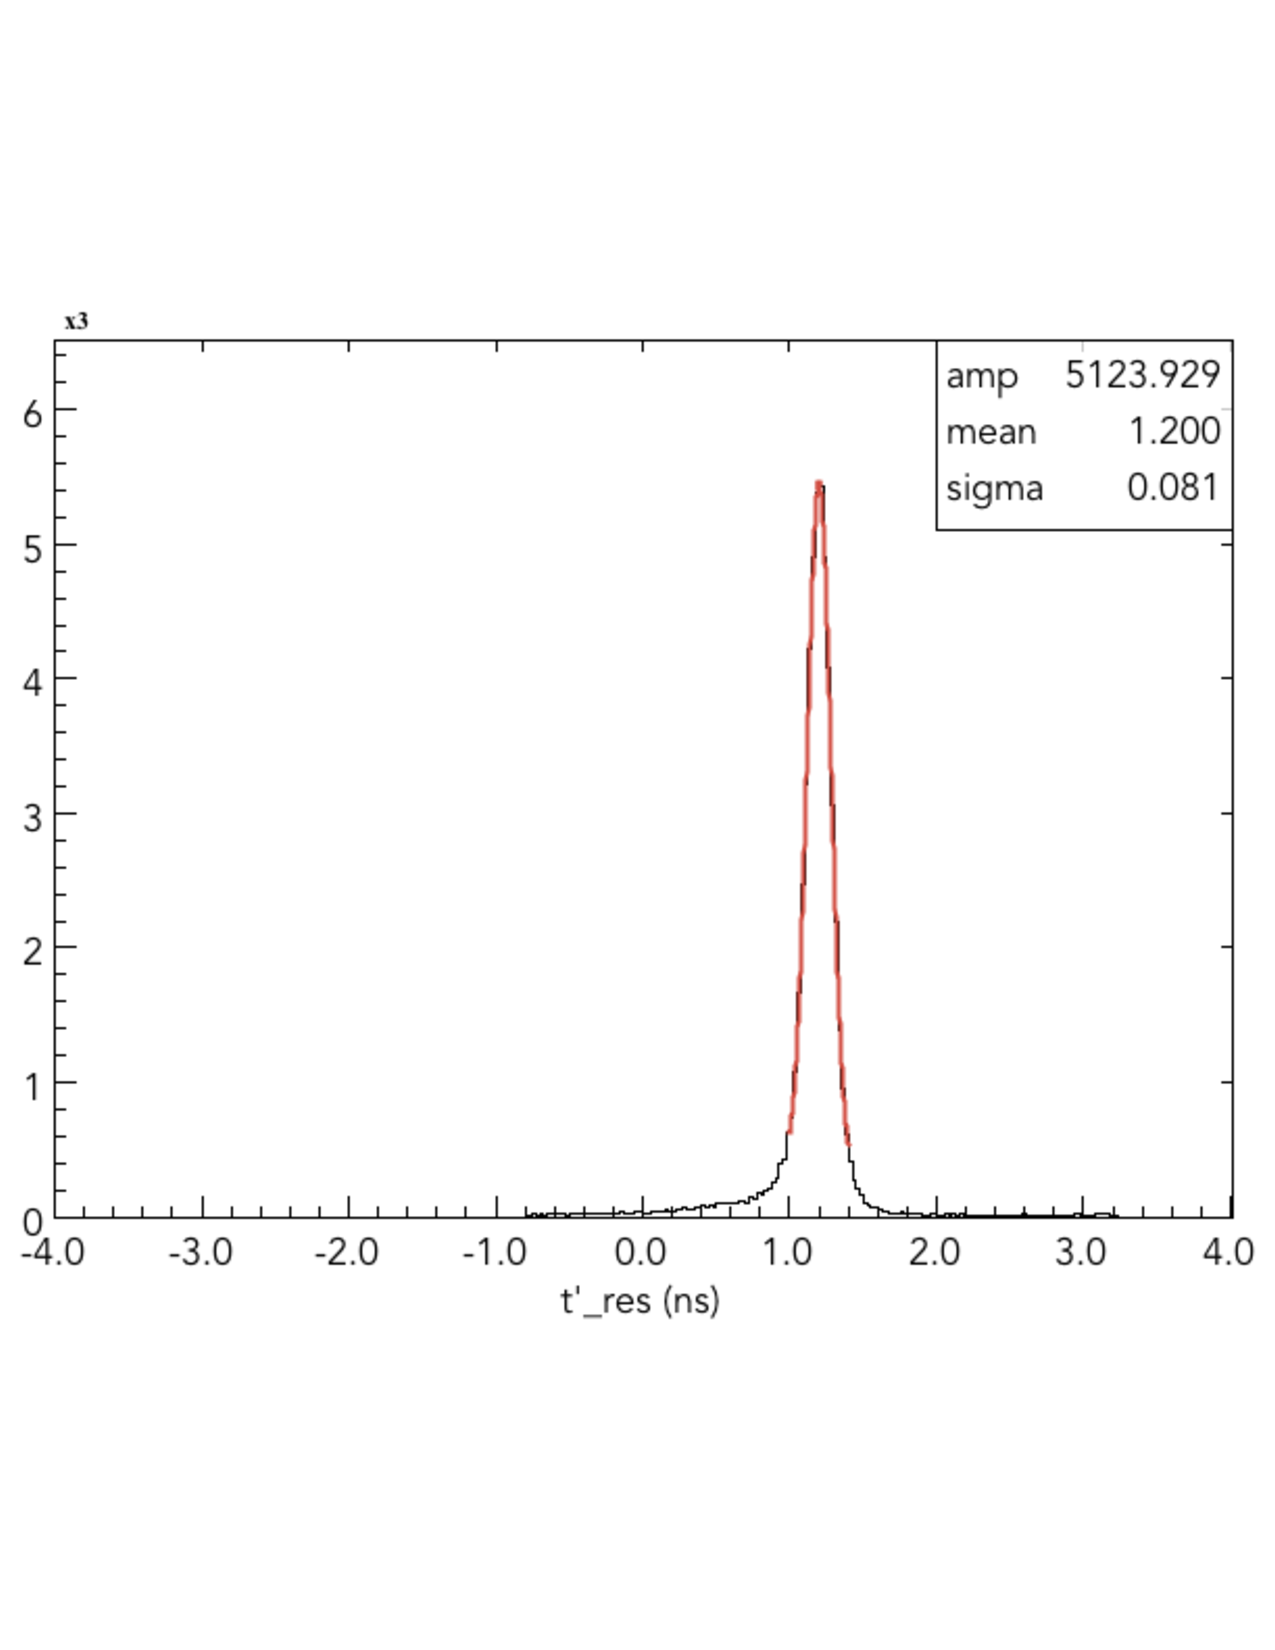
\includegraphics[width=0.5\textwidth,natwidth=610,natheight=642]{pics/rfp-plot.pdf}}}
\end{picture} 
\caption{(Color Online) Distribution of the CTOF hit times from beam data traced back to the vertex relative
to the RF (ns) for one representative CTOF counter with the Gaussian plus background fit overlaid to determine
the counter RF offset and the effective counter timing resolution.}
\label{rfp-plot}
\end{figure}
%%%%%%%%%%%%%%%%%%%%%%%%%%%%%%%%%%%%%%%%%%%%%%%%%%%%%%%%%%

After the fine timing offset calibration, the counter timing is precisely aligned modulo $T_{RF}$. The next
step in the CTOF timing calibration is to fix the measured hit times for all counters to the specific RF bunch
associated with the event. These coarse timing offsets (called P2P for paddle-to-paddle) are determined
using coincidences of charged particle tracks with one track in the forward direction hitting an FTOF
counter and one track in the central detector hitting a CTOF counter. The offsets for each counter are
computed using the time difference:

\begin{equation}
t_{P2P} = t_{vert}^1 - t_{ST}^2,
\end{equation}

\noindent
where,

\begin{equation}
t_{vert}^i = \overline{t}_{hit}^i - \frac{L}{\beta c}.
\end{equation}

\noindent
Here $t_{ST}$ is the event start time determined using the forward-scattered electron each event. The
event start time is determined using the Forward Time-of-Flight system. Therefore the CTOF timing
calibrations can proceed only after the FTOF timing calibrations have been completed. The algorithm
adjusts the vertex time differences over all counters to set them to zero. The coarse time offsets
represents a single parameter for each counter that is restricted to values of $n \cdot T_{RF}$, with
$n = 0, \pm 1, \pm 2, ...$.

Fig.~\ref{p2p-plot} shows the $t_{P2P}$ distribution for one representative CTOF counter. As expected,
the histogram is dominated by events in a single channel (of width $T_{RF}$) centered about $T_{RF} = 0$.
As these constants are predominantly determined by the fixed system cable lengths, the constants primarily
reflect the differences in the signal propagation times along the signal cables.

%%%%%%%%%%%%%%%%%%%%%%%%%%%%%%%%%%%%%%%%%%%%%%%%%%%%%%%%%%
\begin{figure}[htbp]
\vspace{2.4cm}
\begin{picture}(50,50) 
\put(95,-73)
{\hbox{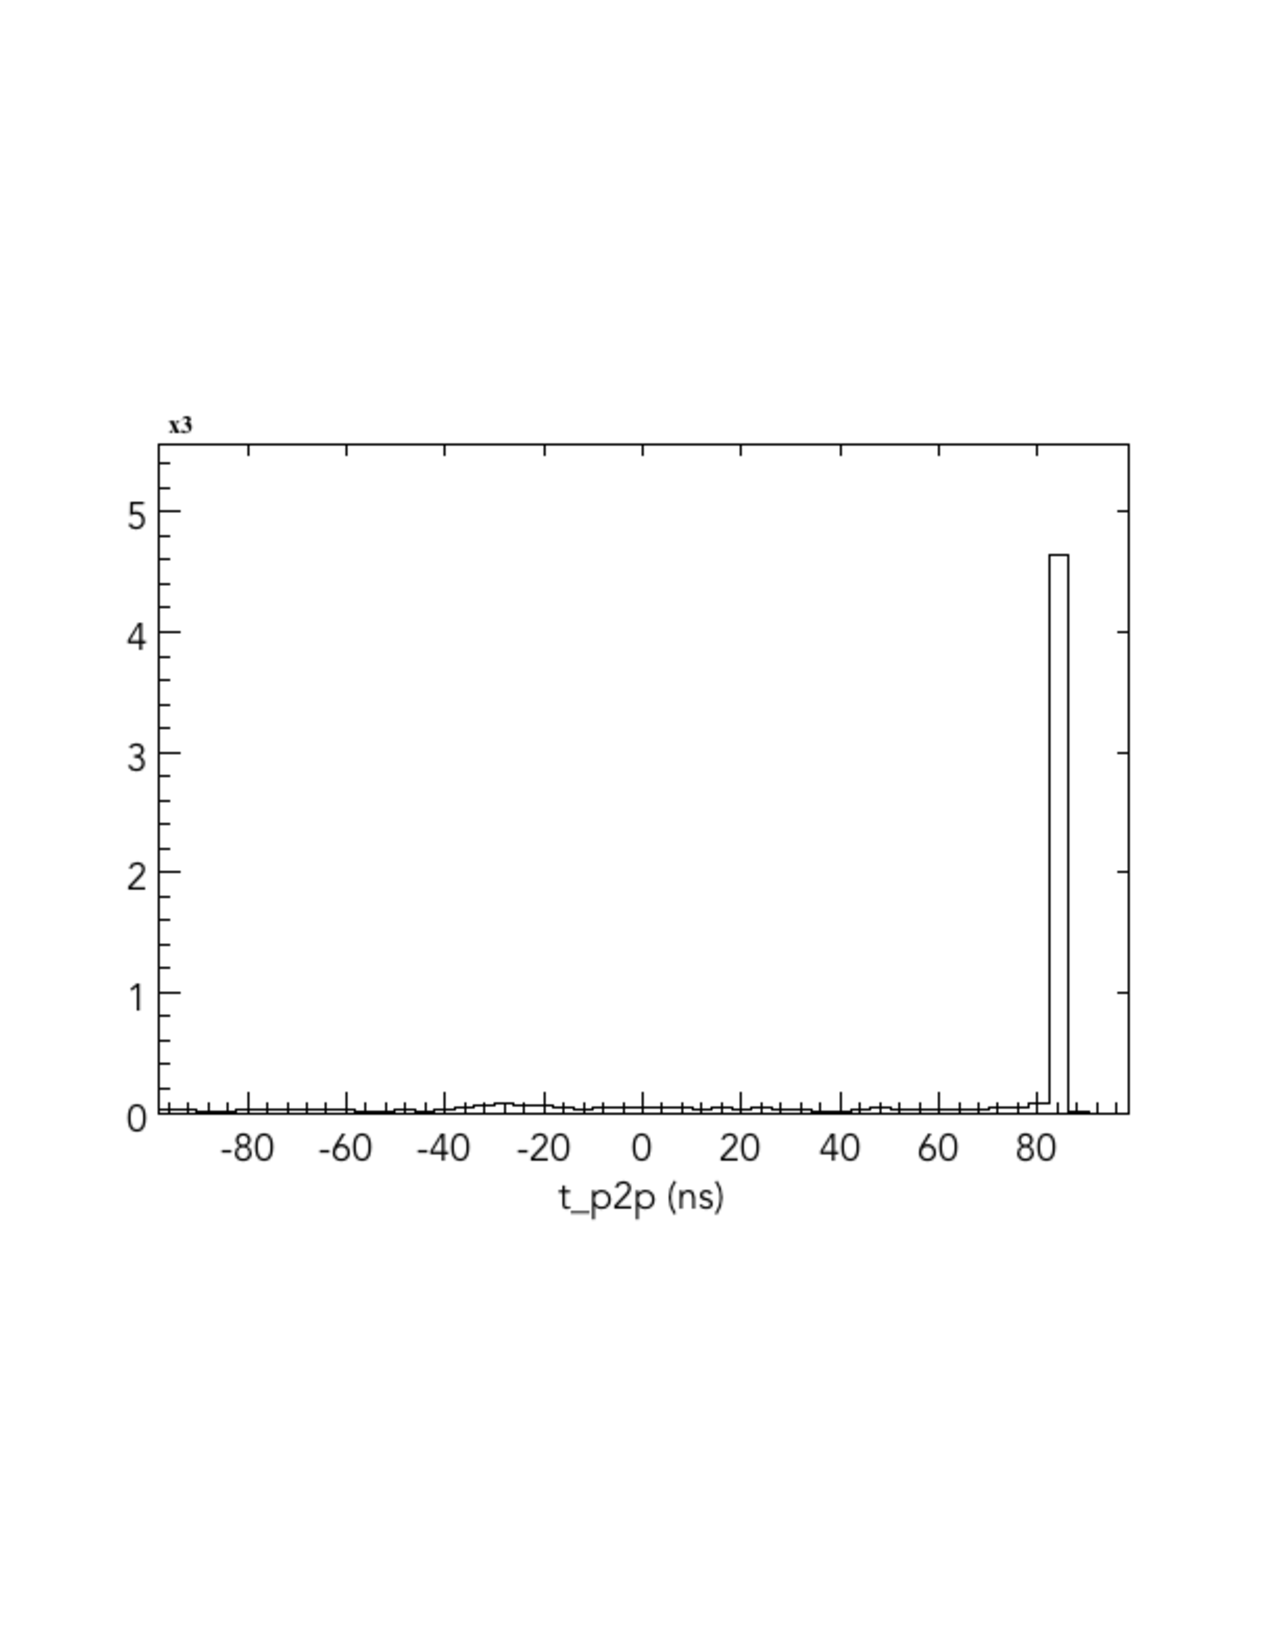
\includegraphics[width=0.50\textwidth,natwidth=610,natheight=642]{pics/p2p-plot1.pdf}}}
\end{picture} 
\caption{Distribution of the vertex time differences (ns) for tracks in a single representative CTOF
counter compared to the event start time determine from the FTOF system. As this plot has been
made after the timing calibrations of the FTOF system have been completed, the dominant bin in this
distribution at 80 ns, gives the P2P offset for this CTOF counter. The histogram is sorted in bins of
$T_{RF}$.}
\label{p2p-plot}
\end{figure}
%%%%%%%%%%%%%%%%%%%%%%%%%%%%%%%%%%%%%%%%%%%%%%%%%%%%%%%%%%

\subsubsection{TDC Calibration}
\label{sec-tdccal}

The final calibration step is the calibration of the TDCs. This calibration is a single constant for each
TDC channel in the system that converts the measured TDC channel bin into time. The nominal TDC
LSB is 25~ps for the CAEN VX1290N TDC units employed for the CTOF readout (see
Section~\ref{sec-elec}).

The calibration is completed by fitting the PMT time residuals vs. TDC channel separately for the times
from the upstream and downstream PMTs using a linear function. The TDC calibration is the value that fixes
the slope of $t_{res}'$ to be zero. Fig.~\ref{tdc-plot} shows the distribution of $t_{res}'$ vs. TDC for a
representative CTOF PMT. Any bin-to-bin $\Delta t$ variations reflect remaining integral non-linearities
in the measured TDC compensation tables (see Section~\ref{sec-elec}). At the present time a single
conversion constant of CONV = 23.45~ps/channel is employed for the CTOF system TDCs.

%%%%%%%%%%%%%%%%%%%%%%%%%%%%%%%%%%%%%%%%%%%%%%%%%%%%%%%%%%
\begin{figure}[htbp]
\vspace{4.2cm}
\begin{picture}(50,50) 
\put(90,-60)
{\hbox{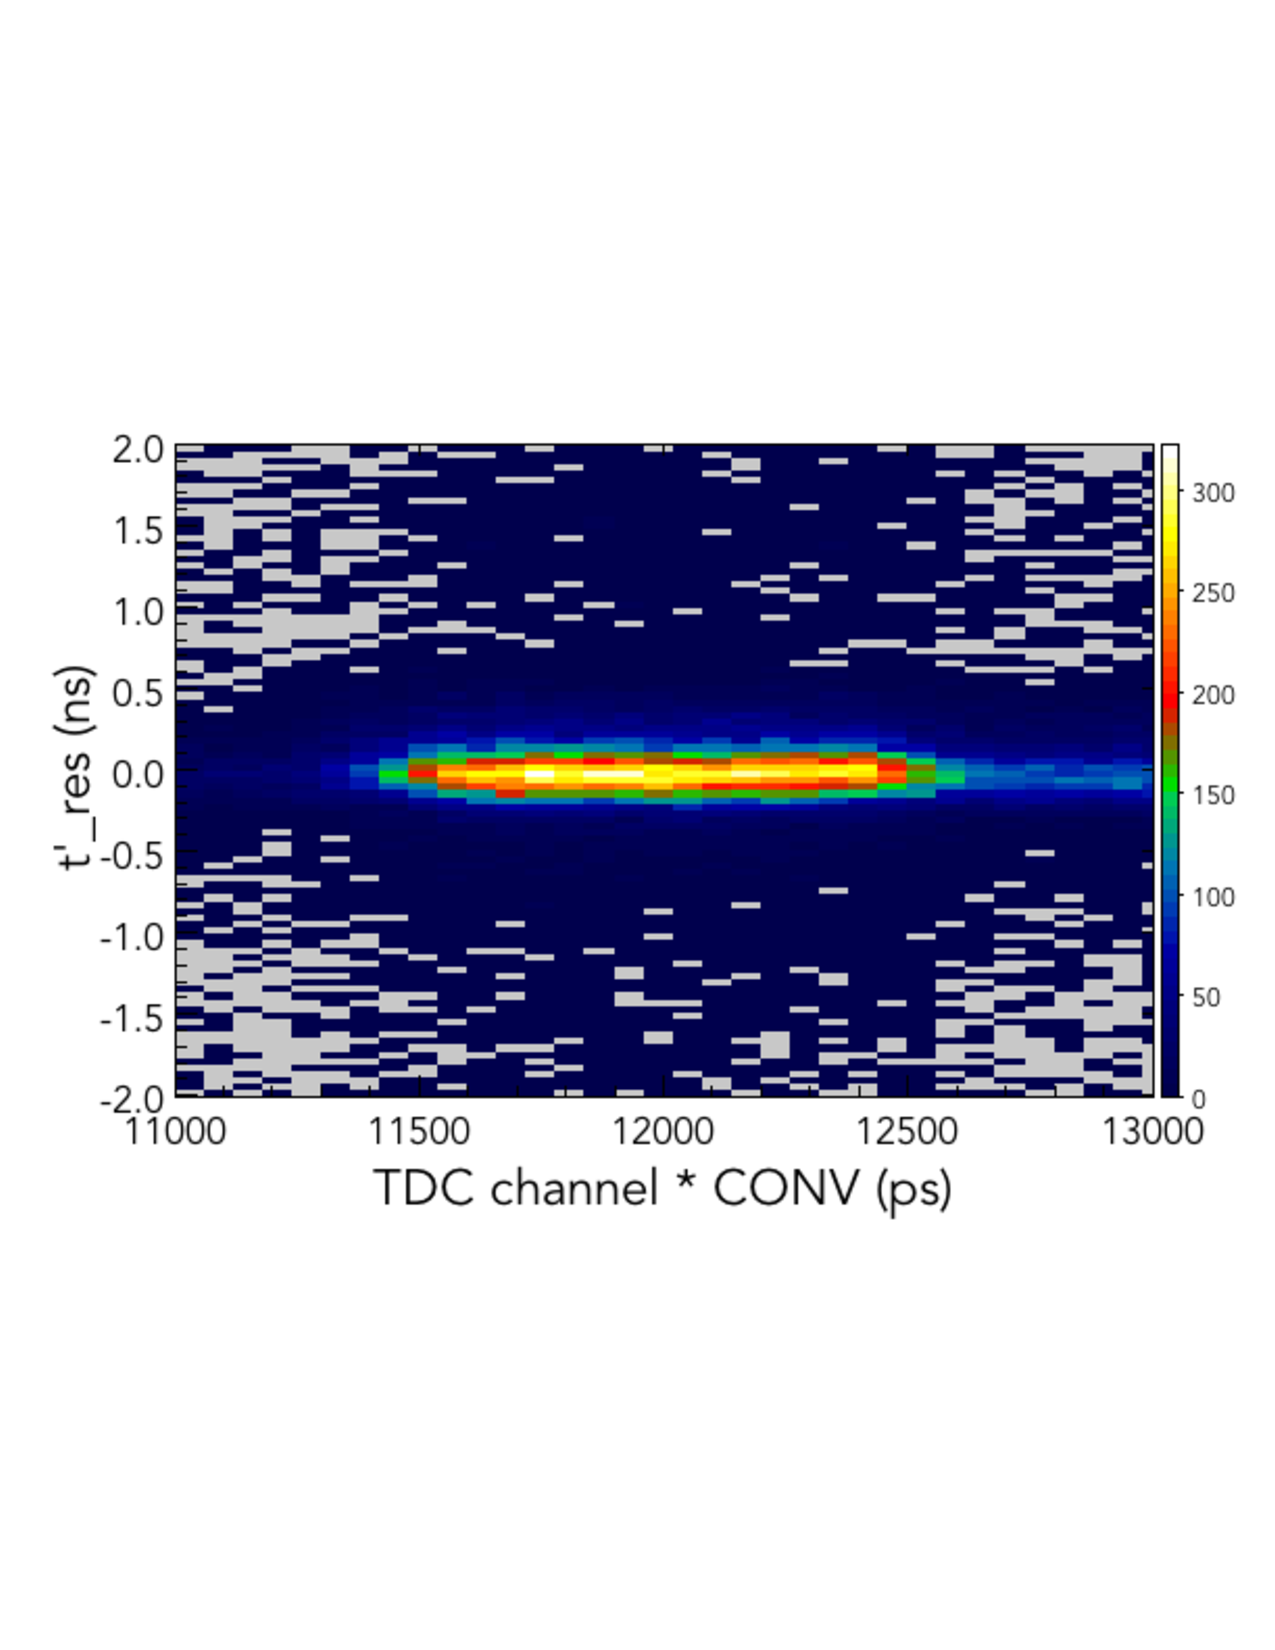
\includegraphics[width=0.55\textwidth,natwidth=610,natheight=642]{pics/tdc-plot.pdf}}}
\end{picture} 
\caption{(Color Online) Distribution of $t_{res}'$ (ns) vs. TDC channel * CONV (ps) for one
representative CTOF PMT. The TDC conversion constant for each channel is that which forces
the slope of a linear fit to be zero.}
\label{tdc-plot}
\end{figure}
%%%%%%%%%%%%%%%%%%%%%%%%%%%%%%%%%%%%%%%%%%%%%%%%%%%%%%%%%%

The CAEN TDCs used for the CTOF are readout with a 24~ns clock strobed so that all TDC times are
referenced to an edge of this clock. The CLAS12 trigger comes on the edge of a clock with a period of
4~ns and the TDC stop will not occur until the next 24~ns clock edge. The use of these two different
clocks introduces a delay between the trigger and the TDC stop given by $n \cdot 4$~ns, with
$n = 0 \to 5$ (referred to as the six-fold TDC cycle ambiguity) where $n$ is the phase. A TDC jitter
correction is made to define the value of the phase $n$ that is valid for the entire data run.

The average hit time resolution for the CTOF from the TDCs is $\sim$70~ps and that from the CTOF
FADCs given the rapid fall time of the fast PMT signals that provide for only 2-3 samples on the falling
edge is only $\sim$1~ns. A matching requirement of 10~ns between the TDC time and the FADC time is
employed during event reconstruction. While this matching requirement still needs to be tuned further,
at the current time is reasonably efficient at allowing the FADC hits to be matched with the TDC hits.
This is important as due to the different thresholds on the discriminators and the FADCs, the number
of entries in the hits lists are up to a factor of two different. The matching criteria is also essential
in order to assign the correct ADC information to the hit that directly uses the measured ADC but also
for the energy loss computation.

\subsubsection{Counter Time Resolutions}
\label{tres-beam}

The effective time resolutions for each counter determined during the fine timing alignment step
discussed in Section~\ref{sec-talign} are shown in Fig.~\ref{eff-tres}. These measurements were
taken after complete calibrations of the CTOF system from a beam data run with 10.6~GeV electrons
incident on a liquid-hydrogen target. The time resolution displayed here represents the quality of the
overall CLAS12 calibrations at the current time. The results are based on calibration procedures that
are not yet fully optimized, as well as uncertainties in the momentum, track path length, and event vertex
from the forward and central track reconstruction. It is also important to mention that studies of the
CLAS12 subsystem detector alignment based on survey data and based on zero-field straight track data
are in progress. Misalignments of the detector affect the quality and accuracy of the reconstruction.
When these are accounted for their contribution to the resolution function is reduced.

Nevertheless the time resolutions already achieved are close to system design specifications outlined in
Section~\ref{sec:overview} and shown in Table~\ref{spec-table}. With these resolutions, the quality of the
particle identification in the Central Detector of CLAS12 allows the experimental program in Hall~B to reach
its goals. As further operating experience with CLAS12 is gained, we expect to realize further modest but
important improvements in the CTOF timing resolution that will allow $\pi/K$, $\pi/p$, and $K/p$ separation
in the Central Detector of CLAS12 to be pushed to higher momenta than currently seen.

%%%%%%%%%%%%%%%%%%%%%%%%%%%%%%%%%%%%%%%%%%%%%%%%%%%%%%%%%
\begin{figure}[htbp]
\vspace{3.4cm}
\begin{picture}(50,50) 
\put(70,-185)
{\hbox{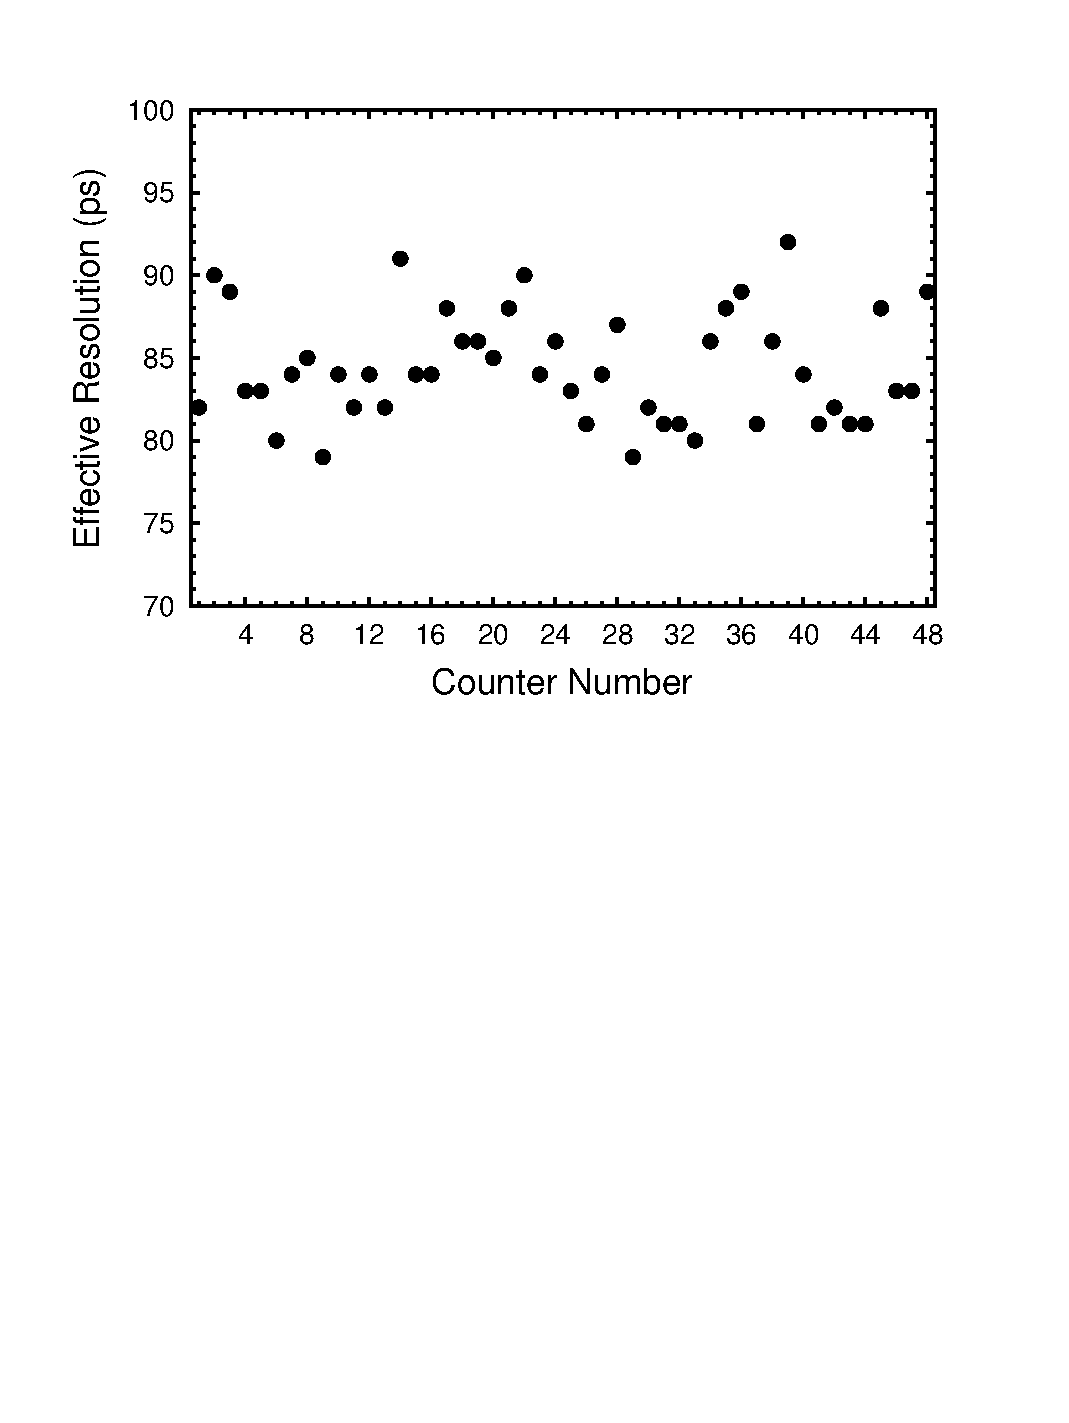
\includegraphics[width=0.8\textwidth,natwidth=610,natheight=642]{pics/res-beam.pdf}}}
\end{picture} 
\caption{The measured effective time resolution (ps) vs. counter number for each of the CTOF counters
from beam data for a 10.6~GeV electron beam incident upon a liquid-hydrogen target.}
\label{eff-tres}
\end{figure}
%%%%%%%%%%%%%%%%%%%%%%%%%%%%%%%%%%%%%%%%%%%%%%%%%%%%%%%%%

Note that as discussed in the Section~\ref{sec:design} introduction, the final CTOF counter resolutions
shown in Fig.~\ref{eff-tres} are listed as effective timing resolutions as they include additional smearing
effects beyond that included in the resolutions discussed and shown in Section~\ref{sec-bench} determined
from the cosmic ray test stand. The contributions from all non-CTOF sources to the effective resolution
effectively adds $\sim$50~ps of smearing in quadrature with the intrinsic CTOF system resolution.

\subsubsection{Hit Times and Clusterization}
\label{cluster}

The reconstructed CTOF counter hit times need to account for the time delays along the readout
path that include the PMT and voltage divider signal transit times, and the signal propagation times along
the signal cables and the electronics. Full details on the CTOF reconstruction in terms of reconstructed hit
times and energy, the reconstruction algorithm, the time, energy, and coordinate uncertainties, and
the hit clustering and matching algorithms are provided in Ref.~\cite{ctof-recon}.

The track hit times reconstructed from the readout of the upstream and downstream PMTs are given by:

\begin{equation}
t_{U,D} = (CONV \cdot TDC_{U,D}) \mp \frac{C_{UD}}{2} + C_{RF} + C_{p2p},
\end{equation}

\noindent
where $CONV$ is the TDC channel to time conversion factor, $TDC$ is the measured TDC value relative
to the trigger signal, $C_{UD}$ is the time shift to center the TDC difference distribution relative to the
track coordinate about 0, and $C_{RF}$ and $C_{p2p}$ are the time shifts to align all of the counter times
with respect to the RF and to each other, respectively.

The hit times of the passing charged particle relative to the trigger signal can be determined separately 
from the times $t_U$ and $t_D$ measured by the upstream and downstream PMTs, respectively, and are
given by:

\begin{equation}
t_{hit}^{U,D} = t_{U,D} - \frac{d^{CVT}_{U,D}}{v_{eff}},
\end{equation}

\noindent
where $d^{CVT}_{U,D}$ are the distances from the track hit point along the bar relative to the end of the
bar as determined by the central tracker. The average CTOF hit time is then given by:

\begin{equation}
\bar{t}_{hit} = \frac{1}{2} ( t_{hit}^U + t_{hit}^D ) = \frac{1}{2} \left[ t_U + t_D - \frac{L}{v_{eff}} \right].
\end{equation}

The output from the FADCs is also used as part of the CLAS12 level-1 trigger. Signals in CTOF above
the FADC threshold of $\sim$1~MeV are used to set a trigger bit that defines charged hadrons in the
CLAS12 Central Detector. Signals from the CTOF system are also used to provide an effective charged
particle veto for the detection of neutrals in the neutron detector radially outward from CTOF. While high
resolution timing measurements are the primary role of the CTOF system for charged particle identification
in the central direction of CLAS12, the pulse height information from the FADCs is also employed for energy
loss measurements to provide an independent means for identification of slow particles. In addition, pulse
fitting techniques are employed using the FADC pulse shape to determine the hit time of the track that is
matched to the TDC time to better ensure matching of the ADC and TDC information in the high rate
operating environment of CLAS12.

Particle trajectories from the target passing through the CTOF barrel can pass through up to two adjacent
counters. To determine the full deposited energy in a given counter layer, a clusterization algorithm is used
to match the CTOF counter hits with the track trajectory at the location of the CTOF array. Neighboring
CTOF hits that match to the trajectory are assigned to be part of a cluster. The assigned cluster energy is
then the sum of the deposited energy in both counters,

\begin{equation}
\label{eclus}
E_{cluster} = \sum_{i=1}^{2} E_{dep}^i.
\end{equation}

\noindent
The relevant path length through the layer is then determined from ray tracing of the central tracker in
the solenoid field. This path length through the CTOF is then used to compute $dE/dx$.

The hit time associated with the cluster in a given layer is based on an energy deposition weighted average
accounting for the time offset between the cluster hits. For the CTOF reconstruction the assigned hit
position in the counter is based on ray tracing of the charged track through the CTOF barrel. For each counter
the hit position is assigned as mid-way between the track entrance point and exit point on the bar. In this way
a cluster hit time is computed as:

\begin{equation}
t_{hit} = t_i \cdot \frac{E_i}{E_{cluster}} + \left(t_{i+1} - \frac{\Delta r_C}{\beta c} \right)
\cdot \frac{E_{i+1}}{E_{cluster}},
\end{equation}

\noindent
where $\beta c$ is the track speed, $\Delta r_C$ is the distance between the hit positions assigned for each
of the counters in the cluster, and $E/E_{cluster}$ is the fraction of the total cluster energy deposited in
each counter in the cluster defined in Eq.(\ref{eclus}).
  
\subsection{Beam Performance}  
\label{sec:beam}

The first in-beam characterization of the CTOF system took place during the Dec. 2017 to Feb. 2018
CLAS12 Engineering Run and subsequently during the first physics production running period that
took place from Mar. - May 2018. During these periods the performance of the CTOF system was
tested at different beam energies (2.2, 6.4, 10.6~GeV), different solenoid magnetic field
strengths and polarities (from 0 field to full field), and over a range of beam-target
luminosities up to twice the nominal planned CLAS12 luminosity of $1 \times 10^{35}$~cm$^{-2}$s$^{-1}$.
In this section the measured scaler rates and PMT currents as a function of beam current are presented,
as well as the reconstruction results and particle identification capabilities relative to the system
specifications based on the current system calibrations.

\subsubsection{CTOF Rates and PMT Currents}

The counting rates during beam operations can be viewed during data taking using the scalers associated
with the FADCs. The threshold applied for these scalers are set at $\sim$1~MeV. During a beam current
scan with a 10.6~GeV electron beam incident upon the 5~cm long liquid-hydrogen target from 5~nA to 75~nA
(corresponding to the nominal design luminosity for CLAS12 $1 \times 10^{35}$~cm$^{-2}$s$^{-1}$) the
average counting rate in the different CTOF counters was studied. The results shown in Fig.~\ref{ctof-rates}
display a reasonably linear behavior. The rates in the downstream PMTs are roughly a factor of two larger
than in the upstream PMTs. Part of this difference is due to the fact that the events seen by the CTOF are
predominantly focused at the downstream end of the counters. Therefore the average path length for light to
travel is longer to the upstream PMTs and the rate difference is due to the longer path length of light attenuation.
However, the likely larger effect is believed to be due to incident radiation on the downstream light guides from
splashback from the entrance to the beamline M{\o}ller cone and the copious conversion of $\pi^0$ mesons in the
region about the target. This radiation generates significant Cherenkov light in the light guides that is seen by the
downstream PMTs and not by the upstream PMTs.

%%%%%%%%%%%%%%%%%%%%%%%%%%%%%%%%%%%%%%%%%%%%%%%%%%%%%%%%%
\begin{figure}[htbp]
\vspace{4.3cm}
\begin{picture}(50,50) 
\put(55,-70)
{\hbox{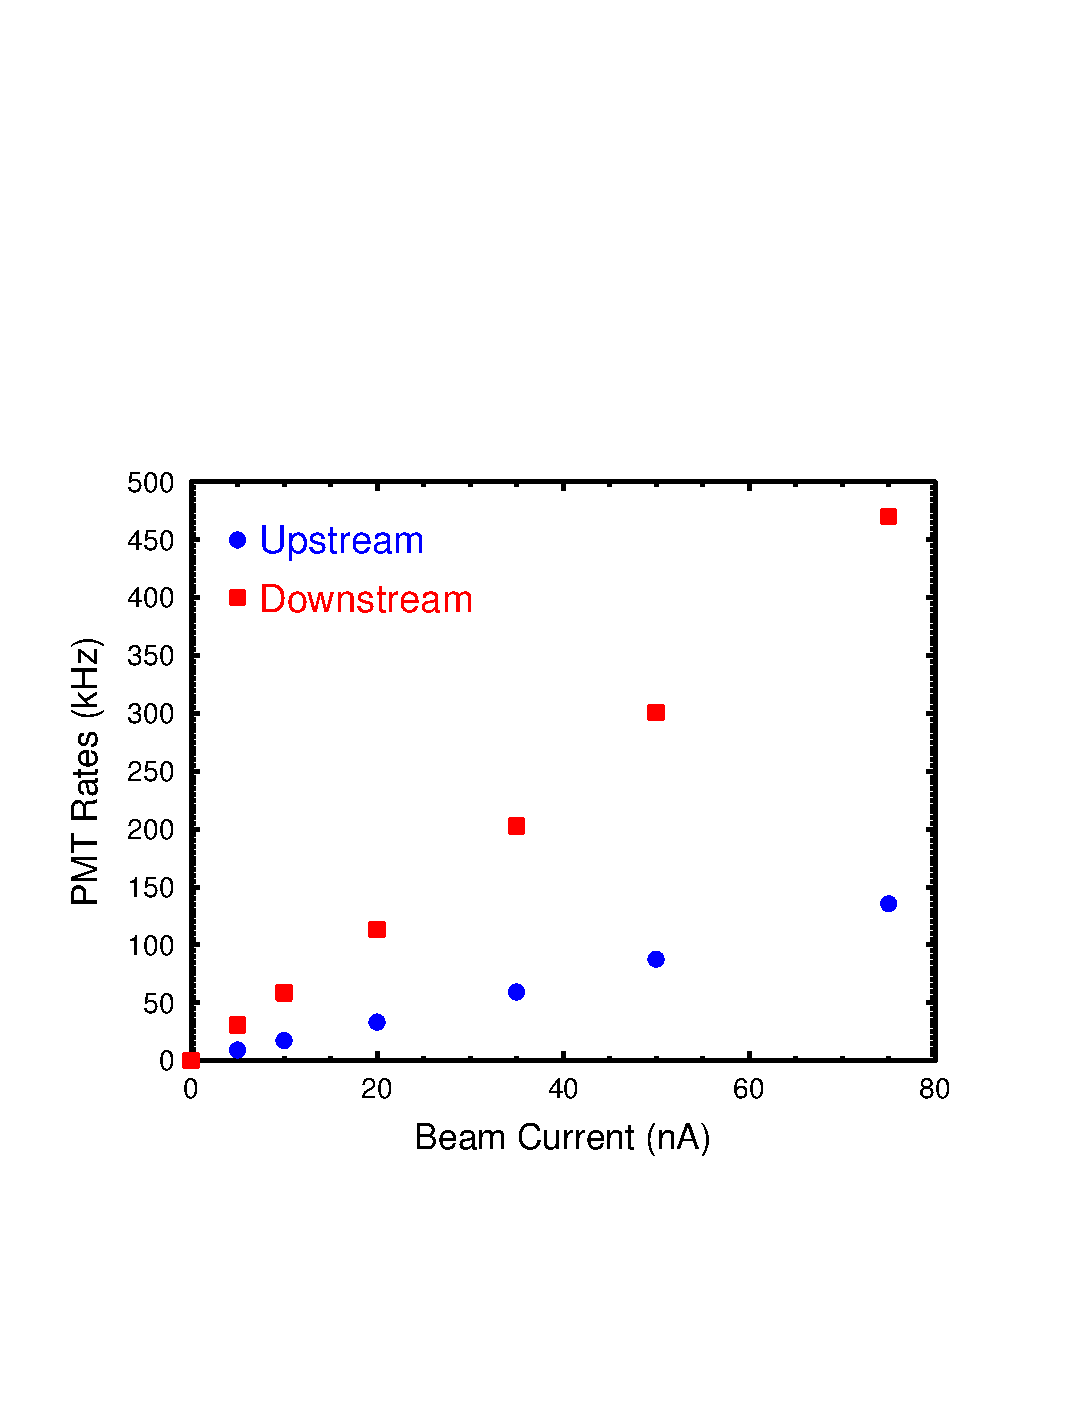
\includegraphics[width=0.8\textwidth,natwidth=610,natheight=642]{pics/rates-ctof.pdf}}}
\end{picture} 
\caption{(Color Online) CTOF counter rates (kHz) for 11~GeV electrons on a liquid-hydrogen target at a beam
current (nA). The nominal operating luminosity of CLAS12 of $1 \times 10^{35}$~cm$^{-2}$s$^{-1}$ corresponds
to a beam current of $\sim$75~nA.}
\label{ctof-rates}
\end{figure}
%%%%%%%%%%%%%%%%%%%%%%%%%%%%%%%%%%%%%%%%%%%%%%%%%%%%%%%%%

Studies using the CLAS12 GEANT-4 Monte Carlo suite called gemc~\cite{gemc} at the full nominal luminosity
indicate that the total integrated rates (hadronic and neutral) for particles that deposit energy greater than
1~MeV in the counters is $\sim$100~kHz/counter and the nominal PMT currents for all incident radiation on the
counter (i.e. with no energy threshold) are $\sim$30-40~$\mu$A~\cite{ctof-cn2018}. Fig.~\ref{ctof-mc} shows
the Monte Carlo results for the CTOF counter rates as a function of track momentum for different particle species.

%%%%%%%%%%%%%%%%%%%%%%%%%%%%%%%%%%%%%%%%%%%%%%%%%%%%%%%%%
\begin{figure}[htbp]
\vspace{3.9cm}
\begin{picture}(50,50) 
\put(70,-75)
{\hbox{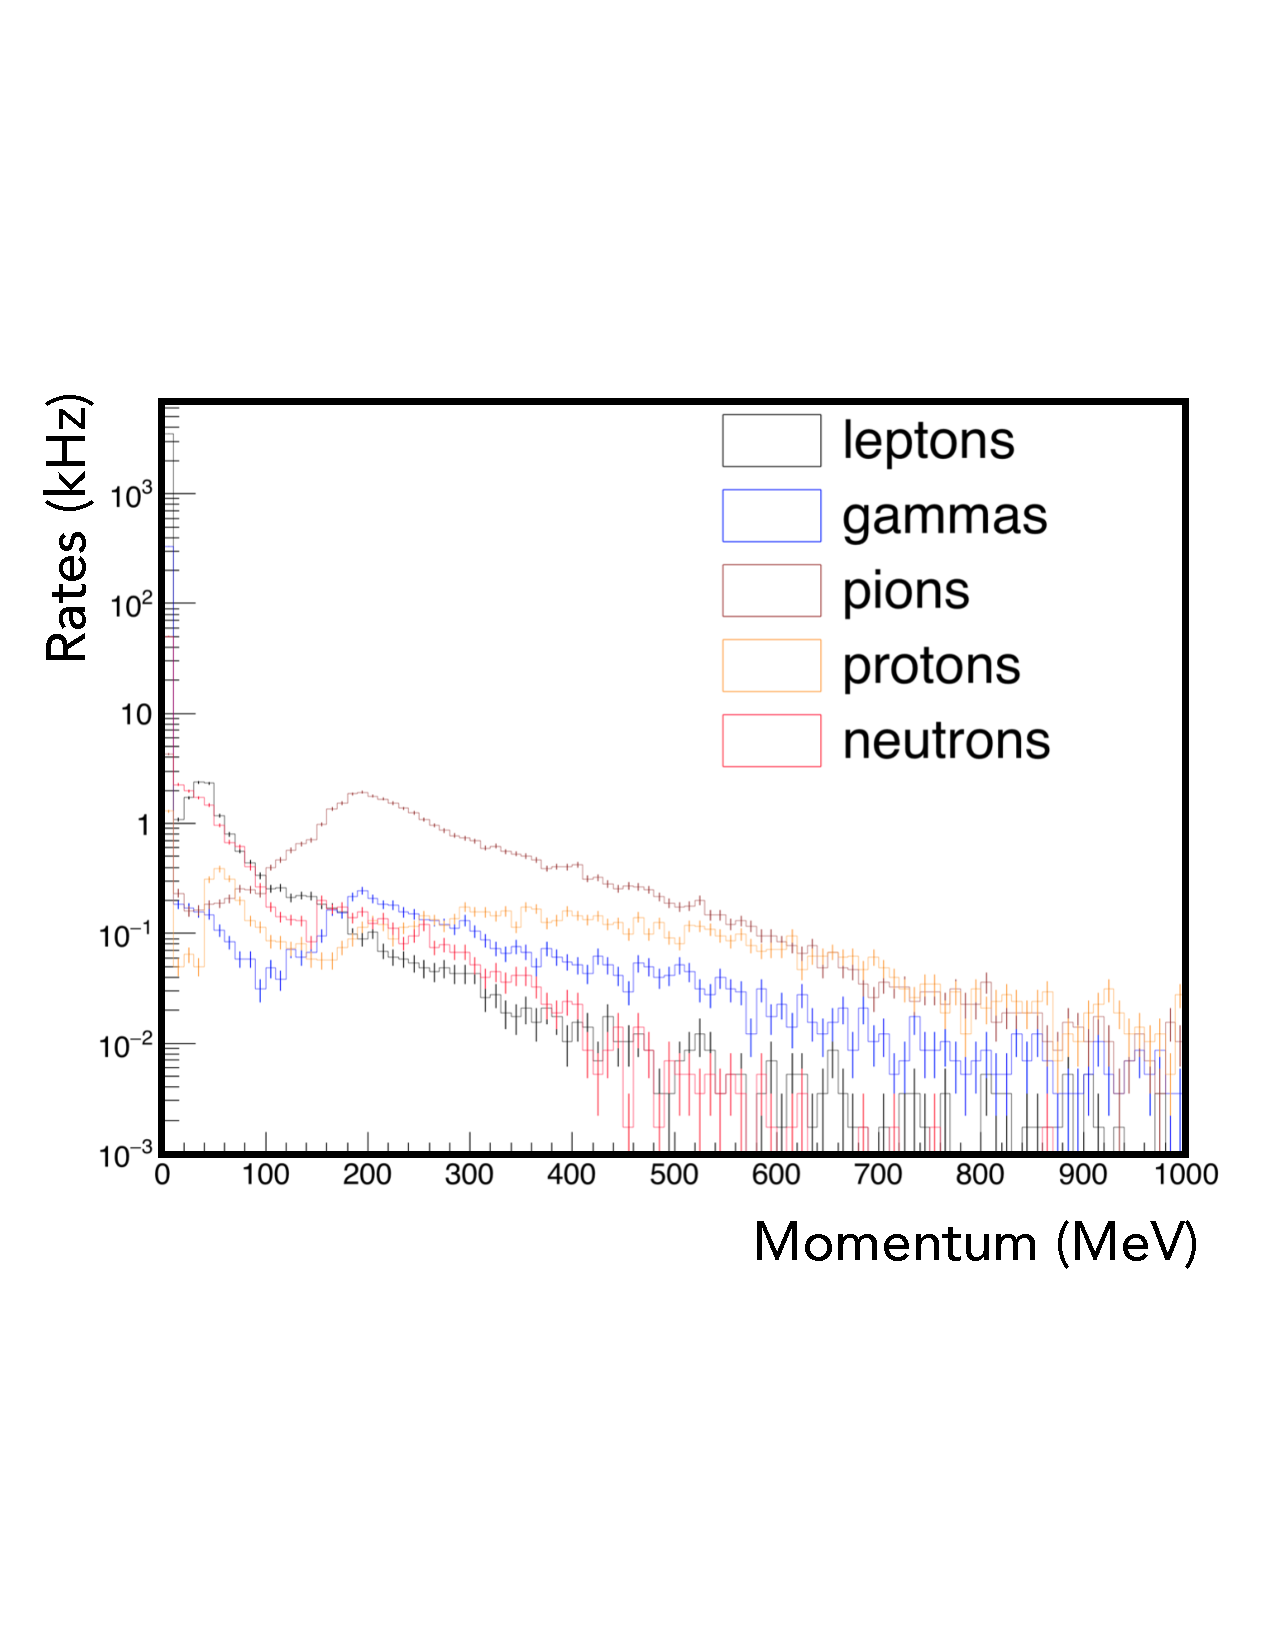
\includegraphics[width=0.60\textwidth,natwidth=610,natheight=642]{pics/ctof-mc-plot.pdf}}}
\end{picture} 
\caption{(Color Online) CLAS12 Monte Carlo calculations for 11 GeV electrons on a liquid-hydrogen target at
a luminosity of $1 \times 10^{35}$~cm$^{-2}$s$^{-1}$ showing CTOF rates per counter as a function of particle
momentum for leptons (black), photons (blue), charged pions (brown), protons (gold), and neutrons (red).}
\label{ctof-mc}
\end{figure}
%%%%%%%%%%%%%%%%%%%%%%%%%%%%%%%%%%%%%%%%%%%%%%%%%%%%%%%%%

From our GEANT-4 Monte Carlo studies, the response of the CTOF with an 11~GeV electron beam incident
upon a 5~cm liquid-hydrogen target has been studied in detail~\cite{ctof-cn2018}. These studies have been
carried out at a beam current of 75~nA corresponding to the full nominal design luminosity of CLAS12 of
$1 \times 10^{35}$~cm$^{-2}$s$^{-1}$. The results of these studies showed that for each CTOF counter the
incident rate of all charged and neutral particles is 4~MHz of which $\sim$97\% is photons and leptons.
With a 1~MeV energy deposition threshold in the CTOF counters to match that applied to the hardware, the
rate of charged and neutral particles is $\sim$130~kHz/counter, half of which is leptons and photons and
half is hadronic. Including attenuation effects along the scintillation bar and light guides, the measured counter
rates at the PMTs are $\sim$110~kHz (upstream) and $\sim$120~kHz (downstream). The predictions for
the upstream PMTs match well what is seen in direct measurements during beam operations. However, the
predictions for the downstream PMTs are a factor of three lower than the direct measurements. This is likely
due to the fact that in the simulation the CTOF light guides are not active materials in which events that
generate Cherenkov light in the light guides (see remarks above) are modeled or included.

In actuality it is not the event rate that defines the luminosity limit of the CTOF system, but the actual
PMT anode currents, which are limited to $\sim$200~$\mu$A (see Section~\ref{divider}). The average
PMT current is directly proportional to the average number of photoelectrons $\langle N_{phe} \rangle$
created at the photocathode by the scintillation light and the average incident charged particle event rate
$\langle R \rangle$. This current can be expressed as:

\begin{equation}
\langle i_{PMT} \rangle = \langle N_{phe} \rangle \cdot Q_e \cdot G \cdot \langle R \rangle,
\end{equation}

\noindent
where $Q_e = 1.6 \times 10^{-19}$ C/e is the electron charge, $G$ is the PMT gain, and $R$ is the rate
per bar. Using the expected photoelectron statistics discussed in Section~\ref{sec:npe} at a PMT gain
of 1$\times$10$^6$, the simulations estimated PMT currents of 30-40~$\mu$A at full nominal CLAS12
luminosity. Direct measurements in beam of the PMT anode currents were made as a function of beam
current as shown in Fig.~\ref{pmt-currents}. The measurements are about three times larger than
expectations. The discrepancy is most likely due to the fact that the sampled PMT (randomly chosen on
the upstream end of CTOF) was operating at a gain above 1$\times$10$^6$.

%%%%%%%%%%%%%%%%%%%%%%%%%%%%%%%%%%%%%%%%%%%%%%%%%%%%%%%%%
\begin{figure}[htbp]
\vspace{4.2cm}
\begin{picture}(50,50) 
\put(60,-70)
{\hbox{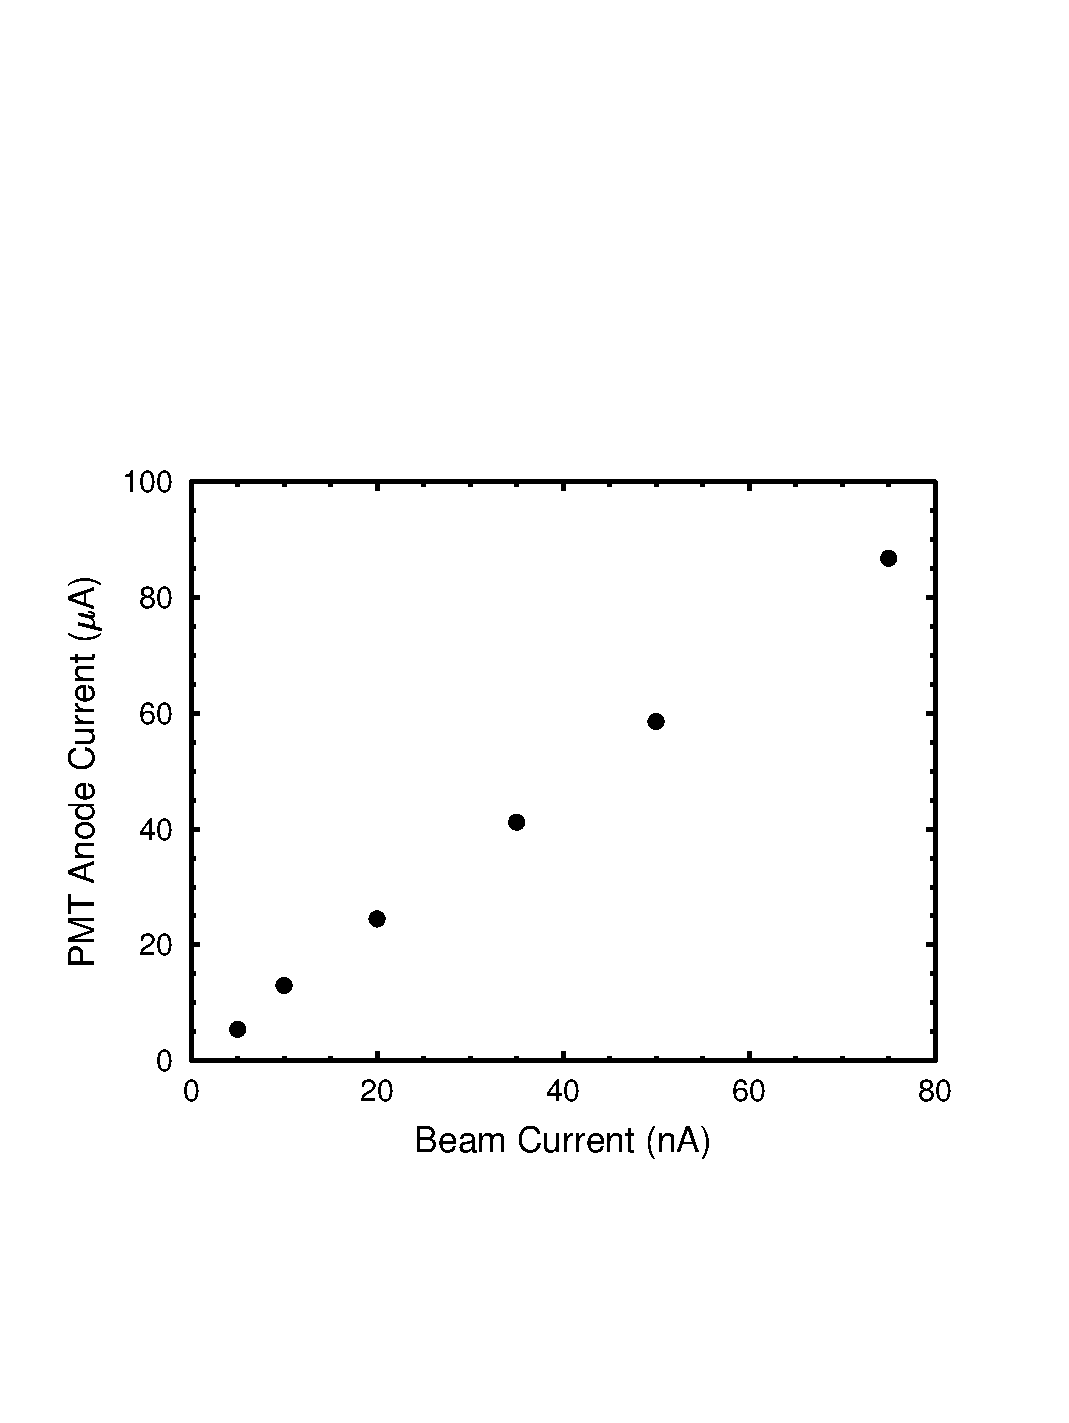
\includegraphics[width=0.8\textwidth,natwidth=610,natheight=642]{pics/full-ctof.pdf}}}
\end{picture} 
\caption{Measurements of the PMT anode current ($\mu$A) for a representative upstream CTOF PMT
as a function of beam current (nA) with a 10.6~GeV electron incident upon a 5~cm liquid-hydrogen target.}
\label{pmt-currents}
\end{figure}
%%%%%%%%%%%%%%%%%%%%%%%%%%%%%%%%%%%%%%%%%%%%%%%%%%%%%%%%%

\subsubsection{Reconstruction Results}

Particle identification in the Central Detector of CLAS12 relies heavily on the combination of measured
charged particle momenta and the flight time from the target to the respective CTOF counters. The
vertex time is determined with respect to the accelerator RF, modulo the RF period $T_{RF}$. The beam
bucket for each event is identified using the flight time of scattered electrons or high momentum pions
detected in the CLAS12 Forward Detector traced back to the interaction point. The FTOF resolution of
$< 200$~ps~\cite{ftof-nim}  allows clear selection of the correct beam bucket. In Fig.~\ref{ctof-pid}
we show the distribution of masses for all reconstructed positively and negatively charged hadrons in CTOF
without any kinematic cuts other than those imposed by the detector acceptance for the data taken with a
10.6~GeV electron beam incident upon a liquid-hydrogen target and after initial calibrations of the CTOF
system. A clear separation of pions and protons can be seen from these data. For these data the $RF$
period was 4.008~ns.

%%%%%%%%%%%%%%%%%%%%%%%%%%%%%%%%%%%%%%%%%%%%%%%%%%%%%%%%%
\begin{figure}[htbp]
\vspace{6.0cm}
\begin{picture}(50,50) 
\put(60,-75)
{\hbox{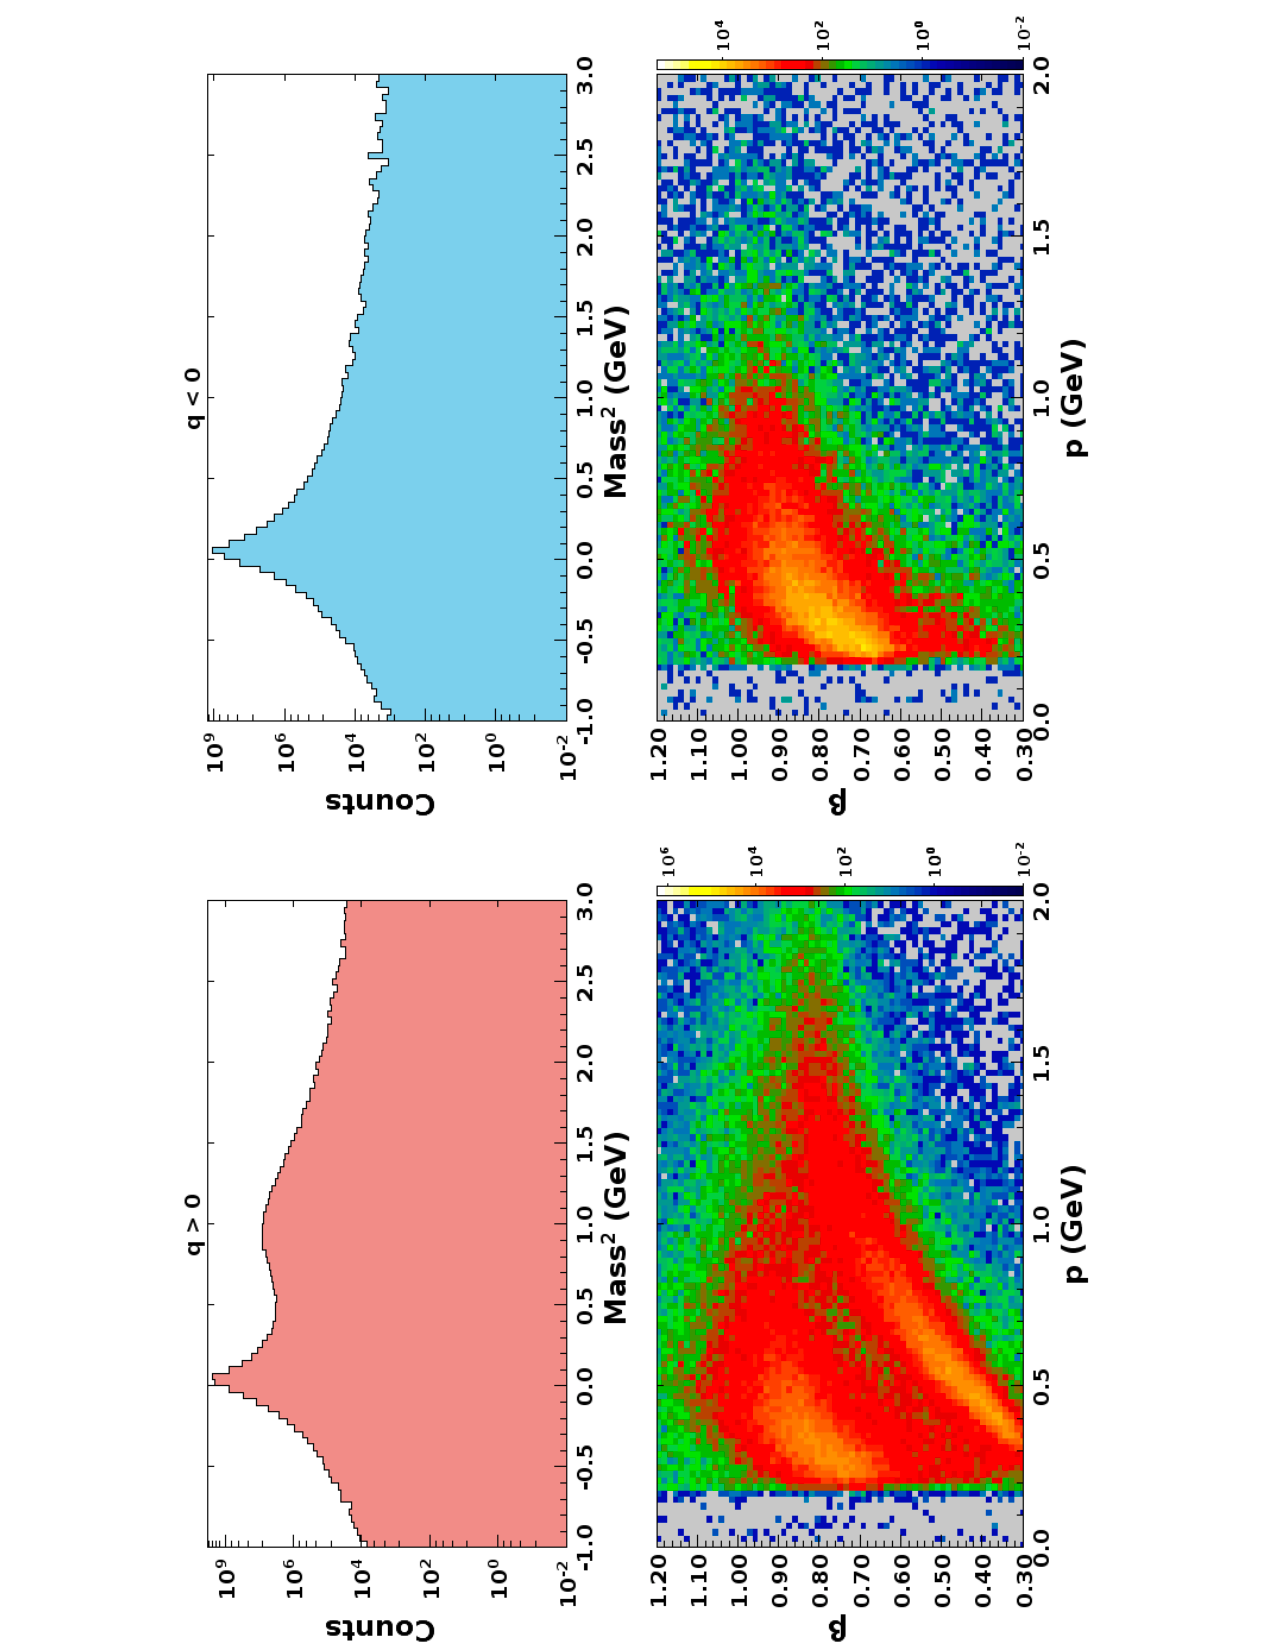
\includegraphics[width=0.7\textwidth,natwidth=610,natheight=642]{pics/ctof-pid.pdf}}}
\end{picture} 
\caption{(Color Online) Reconstructed mass squared (GeV$^2$) and $\beta$ vs. momentum distributions
for positively charged particles (top row) and negatively charged particles (bottom row) for all CTOF
counters from beam data with a 10.6~GeV electron incident on a liquid-hydrogen target.}
\label{ctof-pid}
\end{figure}
%%%%%%%%%%%%%%%%%%%%%%%%%%%%%%%%%%%%%%%%%%%%%%%%%%%%%%%%

Plots of velocity versus momentum are shown in Fig. \ref{ctof-pid} for positively and negatively charged
particles, displaying the overall particle identification possible with this detector through the separation
of the different particle species. These distributions qualitatively show the particle separation for $\pi/K$,
$\pi/ p$, and $K/p$ vs. momentum as required by the system specifications in Section~\ref{sec:overview}
and Table~\ref{spec-table}.

\section{Summary}
\label{sec:summary}

We have designed and built a time-of-flight system for the CLAS12 Central Detector in Hall~B 
at Jefferson Lab known as the Central Time-of-Flight or CTOF detector. This system consists 
of 48 90-cm-long scintillation bars of a wedge-shaped cross section that form a hermetic barrel
at a radius of 25~cm from the beamline. As the CTOF system is positioned inside of a 5-T
superconducting solenoid, the light is delivered to the PMTs through long light guides to allow the
PMTs to be positioned in reduced field regions where a multi-layer shield system reduces the
magnet fringe fields to the level of 0.2~G at the PMT photocathode. The scintillation bars are read
out at each end. The detector was designed to have an intrinsic time resolution of about 65~ps and
this level of performance has been achieved. With these timing resolutions the CTOF system can
separate $\pi/K$ to 2.8~GeV, $K/p$ to 4.8~GeV, and $\pi/p$ to 5.4~GeV with 4$\sigma$ separation
with up to an order of magnitude difference in the relative yields.  The specifications are sufficient to
meet to meet the particle identification requirements in the forward direction for the full CLAS12
physics program. The performance of the CTOF system was verified in extensive bench studies in our
cosmic ray test stands as well as after installation in the first beam runs with the CLAS12 system in
the period from Dec. 2017 to May 2018. 

\ack

We benefited greatly from useful discussions with and assistance from Sergey Boyarinov, Chris Cuevas,
Ralf Gothe, Chris Keith, Eugene Pasyuk, Cole Smith, Elton Smith, Maurizio Ungaro, and Veronique Ziegler.
We thank the Hall~B technical crew for their efforts during counter installation and cabling. Finally, we
thank the summer students that contributed to component assembly and testing for this system.
This work was supported in part by DOE Contract \#DE-AC05-84ER40150.

\newpage

\begin{thebibliography}{99}

\bibitem{clas-nim}
B.A. Mecking {\it et al.}, Nucl. Inst. and Meth. {\bf A503}, 513 (2003).

\bibitem{clas12-nim}
V.D. Burkert {\it et al.}, to be published in Nucl. Inst. and Meth. A, (2020).
  
\bibitem{gemc}
CLAS12 GEANT4 Monte Carlo suite {\it gemc}, http://gemc.jlab.org.

\bibitem{tof-nim}
E.S. Smith {\it et al.}, Nucl. Inst. and Meth. {\bf A432}, 265 (1999).

\bibitem{ftof-nim}
D.S. Carman {\it et al.}, to be published in Nucl. Inst. and Meth. A, (2020).

\bibitem{baturin-2009}
V. Baturin {\it et al.}, {\it ``Time Resolution Measurements with the Final Prototype for the 
CLAS12 Central TOF Detector''}, CLAS-Note 2009-001.\\
https://misportal.jlab.org/ul/Physics/Hall-B/clas/viewFile.cfm/2009-001.pdf?documentId=549

\bibitem{geom-note}
V. Baturin and D.S. Carman, {\it ``Central Time-of-Flight Geometry for CLAS12''}, CLAS12-Note 
2016-001.\\
https://misportal.jlab.org/mis/physics/clas12/viewFile.cfm/2016-001.pdf?documentId=25

\bibitem{eljen-ref}
Eljen Technology, 1300 W. Broadway, Sweetwater, TX 79556

\bibitem{bicron-ref}
Saint Gobain Crystals, 12345 Kinsman Road, Newbury, OH 44065

\bibitem{eljen-guide}
Eljen Technology Scintillator Polishing Guide,\\
http://www.eljentechnology.com/images/technical-library/Plastic\_Polishing.pdf

\bibitem{plas-ref}
Plastic-Craft Products Corporation, 744 West Nyack Rd., P.O. Bos K, West Nyack, NY 10994

\bibitem{barbosa06}
F. Barbosa {\it et al.}, {\it ``Status and Further Steps Towards the CLAS12 ``Start''-Counter''},
CLAS-Note 2006-011.\\
https://misportal.jlab.org/ul/Physics/Hall-B/clas/viewFile.cfm/2006-011.pdf?documentId=278

\bibitem{mutch} 
G. Mutchler and Y. Sharabian, {\it ``Wrapping Tests and Monte Carlo Evaluation of a New Highly 
Segmented CLAS Start Counter''}, CLAS-NOTE 2005-008.\\
https://misportal.jlab.org/ul/Physics/Hall-B/clas/viewFile.cfm/2005-008.pdf?documentId=167

\bibitem{3m-ref}
3M Optical Systems, http://www.apioptics.com/pdf/ESR.pdf

\bibitem{ilt-ref}
International Light Technologies, http://www.intl-lighttech.com/

\bibitem{ham-ref}
Hamamatsu Corporation, 360 Foothill Rd., Box 6910, Bridgewater, NJ 08807

\bibitem{r2083-ref}  
Hamamatsu R2083 PMT, http://www.hamamatsu.com/us/en/R2083.html

\bibitem{ham-schem}
Hamamatsu H2431 Assembly, \\
http://www.hamamatsu.com/resources/pdf/etd/PMT\_TPMZ0002E.pdf

\bibitem{burle-ref}
Burle Industries, 1000 New Holland Ave, Lancaster, PA 17601

\bibitem{kichimi}
H. Kichimi {\it et al.}, Nucl. Inst. and Meth. A {\bf 325}, 451 (1993).

\bibitem{baturin06}
V. Baturin {\it et al.}, Nucl. Inst. and Meth. A {\bf 562}, 327 (2006).

\bibitem{bonesini}
M. Bonesini {\it et al.}, Nucl. Inst. and Meth. A {\bf 567}, 200 (2006).

\bibitem{baturin11}
V. Baturin {\it et al.}, {\it ``TOF Resolution Measurements with the CLAS12 Central TOF 
Detector with Fine-Mesh Photomultiplier Tubes''}, CLAS-Note 2011-005.\\
https://misportal.jlab.org/ul/Physics/Hall-B/clas/viewFile.cfm/2011-005.pdf?documentId=633

\bibitem{popov}
V. Popov, Nucl. Inst. and Meth.A {\bf 505}, 316 (2003).

\bibitem{opera}
Opera 3-D magnetic field computations, see http://operafea.com/.

\bibitem{baturin12}
V. Baturin {\it et al.}, Nucl. Inst. and Meth. A {\bf 664}, 11 (2012).

\bibitem{cn2015-003} 
V. Baturin and D.S. Carman, {\it ``Design and Performance Tests of the Dynamical Magnetic Shields 
for the CLAS12 Central Time-of-Flight Detector''}, CLAS12-NOTE 2015-003.\\
https://misportal.jlab.org/mis/physics/clas12/viewFile.cfm/2015-003.pdf?documentId=19

\bibitem{wiener-ref}
Wiener Plein and Baus Corporation,\\
http://www.wiener-d.com/sc/power-supplies/mpod--lvhv/

\bibitem{poisson}
Poisson Superfish program, \\
http://laacg.lanl.gov/laacg/services/download\_sf.phtml

\bibitem{shield-test} 
D.S. Carman, G. Asryan, and A. Ni, {\it ``Central Time-of-Flight Magnetic Shield Performance 
Studies''}, CLAS12-NOTE 2015-004.\\
https://misportal.jlab.org/mis/physics/clas12/viewFile.cfm/2015-004.pdf?documentId=20

\bibitem{bc600-ref}
Bicron BC-600 Optical Cement,\\
http://www.crystals.saint-gobain.com/uploadedFiles/SG-Crystals/Documents/SGC\%20BC600\%20Data\%20Sheet.pdf

\bibitem{dymax}
Dymax 3-20262 UV curing glue, https://www.dymax.com/images/pdf/pds/3-20262.pdf
  
\bibitem{vm2002-ref}
VM-2002 (also called Vikuiti) Enhanced Specular Reflector, \\
http://www.apioptics.com/pdf/ESR.pdf

\bibitem{dupont-ref}
Dupont Tedlar Film,\\
http://www.dupont.com/products-and-services/membranes-films/pvf-films/brands/tedlar-pvf-films.html

\bibitem{ctof-wrapping} 
D.S. Carman, {\it ``Central Time-of-Flight Counter Wrapping Procedures''}, CLAS12-Note 2016-002.\\
https://misportal.jlab.org/mis/physics/clas12/viewFile.cfm/2016-002.pdf?documentId=26

\bibitem{ctof-sh-assy} 
D.S. Carman, {\it ``Central Time-of-Flight Magnetic Shield Attachment Procedures''}, CLAS12-Note 
2016-003.\\
https://misportal.jlab.org/mis/physics/clas12/viewFile.cfm/2016-003.pdf?documentId=27

\bibitem{bc-630}
BC-630 Optical Grease,\\
https://www.crystals.saint-gobain.com/products/assembly-materials
  
\bibitem{ortec-ref}
Ortec 935 Discriminator, \\
http://www.ortec-online.com/products/electronics/fast-timing-discriminators/935

\bibitem{tdc-manual}
CAEN VX1290N TDC Manual,\\
http://www.caen.it/servlet/checkCaenManualFile?Id=12125
  
\bibitem{inl-tables}
E. Jastremski, https://www.jlab.org/Hall-B/ftof/manuals/caen-inl-notes.pdf

\bibitem{fadc-manual}
https://www.jlab.org/Hall-B/ftof/manuals/FADC250UsersManual.pdf
  
\bibitem{epics}
EPICS (Experimental Physics and Industrial Control System),\\ http://www.aps.anl.gov/epics

\bibitem{dsc-cn2016-009}
D.S. Carman, {\it ``Central Time-of-Flight System Bench Testing Results''},\\
CLAS12-Note 2016-009.\\
https://misportal.jlab.org/mis/physics/clas12/viewFile.cfm/2016-009.pdf?documentId=49

\bibitem{agilent-ref}
https://www.jlab.org/Hall-B/ctof/manuals/agilent\_mso-x\_manual.pdf

\bibitem{twalk}
D.S. Carman, {\it ``CLAS12 CTOF Time-Walk Corrections''}, CLAS12-Note 2015-006.\\
https://misportal.jlab.org/mis/physics/clas12/viewFile.cfm/2015-006.pdf?documentId=24

\bibitem{ctof-calib}
D.S. Carman, {\it Description of the Calibration Algorithms for the CLAS12 Central Time-of-Flight System},\\
https://www.jlab.org/Hall-B/ctof/notes/ctof\_calib.pdf

\bibitem{scint-spec}
Eljen Technologies scintillator specifications,\\
http://www.eljentechnology.com/images/technical\_library/Physical\_Constants\_Plastic.pdf

\bibitem{ctof-recon}
D.S. Carman, {\it Central Time-of-Flight Reconstruction for CLAS12},\\
https://www.jlab.org/Hall-B/ctof/notes/ctof-recon.pdf

\bibitem{ctof-cn2018}
V. Burkert, D.S. Carman, L.C. Smith, and M. Ungaro, {\it Study of Tungsten Shielding Before CTOF to Limit
its PMT Currents}, CLAS12-Note 2018-006.\\
https://misportal.jlab.org/mis/physics/clas12/viewFile.cfm/2018-006.pdf?documentId=60
  
%\bibitem{Gi86} 
%R.T. Giles, F.M. Pipkin, and J.P. Wolinski, Nucl. Instr. and Meth. A {\bf 252}, 41 (1986).

%\bibitem{pulser-board}
%JLab Fast Pulser, \\
%http://www.jlab.org/Hall-B/ctof/lms/FastLEDPulser\_Description\_InstructionsDRAFT1.pdf

%\bibitem{gegham}
%G. Asyran, {\it ``Monte-Carlo Simulations of Light Transmission for the CTOF Light Monitoring 
%System''}, CLAS12-Note 2016-007.\\
%https://misportal.jlab.org/mis/physics/clas12/viewFile.cfm/2016-007.pdf?documentId=33

%\bibitem{metrolab-ref}
%http://www.gmw.com/magnetic\_measurements/MetroLab/THM-7025.html

%\bibitem{kuhlen}
%M. Kuhlen, M. Moszynski, R. Stroynowski, E. Wicklund, and B. Milliken, Nucl.  Instr. and Meth.
%{\bf A301}, 223 (1991).

%\bibitem{scint-mat-ref}
%https://www.crystals.saint-gobain.com/sites/imdf.crystals.com/files/documents/bc400-404-408-412-416-data-sheet.pdf

%\bibitem{et-ref}
%ADIT Electron Tubes, 300 Crane St, Sweetwater, TX 79556
  
%\bibitem{photonis}
%Photonis Imaging Sensors, http://www.photonis.com

%\bibitem{kajino}
%T. Yamaoka, F. Kajino, I. Tada, S. Hayashi, {\it Absolute Number Calibration of Photoelectrons of
%Photomultiplier Tubes Using the Nature of Statistical Distribution}, Proceedings of the 28th International
%Cosmic Ray Conference, July 31 - August 7, 2003, editors: T. Kajita, Y. Asaoka, A. Kawachi, Y. Matsubara, and
%M. Sasaki, p. 2871 (2003).

%\bibitem{gemc-cn2017}
%R. De Vita, D.S. Carman, C. Smith, S. Stepanyan, and M. Ungaro, {\it Study of the Electromagnetic Background
%Rates in CLAS12}, CLAS12-Note 2017-016.\\
%https://misportal.jlab.org/mis/physics/clas12/viewFile.cfm/2017-016.pdf?documentId=52

%\bibitem{guide7}
%T. Massam, Guide-7, A general program for evaluating the properties of scintillation and
%Cherenkov counter optical systems, CERN Library (1976).\\
%https://cds.cern.ch/record/117452

\end{thebibliography}

\end{document}
